\paragraph{Abstract for Chapter~\ref{ch:msr3}} Linear Mixed-Effects (LME) models are a fundamental tool for modeling correlated data, 
including cohort studies, longitudinal data analysis, and meta-analysis.  Design and analysis of variable selection methods for LMEs is more difficult than for linear regression because LME models are nonlinear. In this work we 
propose a relaxation strategy and optimization methods that enable a wide range of variable selection methods for LMEs using both convex and nonconvex regularizers, including  $\ell_1$, Adaptive-$\ell_1$, SCAD, and $\ell_0$. 
The computational framework only requires the proximal operator for each regularizer to be available, and the implementation is available in an open source \texttt{python} package \texttt{pysr3}, consistent 
with the \texttt{sklearn} standard. 
The numerical results on simulated data sets indicate that the proposed strategy improves on the state of the art for both accuracy and compute time. 
The variable selection techniques are also validated on a real example using a data set on bullying victimization.

{\it Keywords:}  Mixed effects models, feature selection, nonconvex optimization 
%\vfill
%
%\newpage
%\spacingset{1.5} % DON'T change the spacing!


\section{Introduction}
Linear mixed-effects (LME) models use covariates 
%(also known as predictors or features) 
to explain the variability of target variables in a grouped data setting. For each group, the relationship between covariates and observations is modeled 
using group-specific coefficients that are linked by a common prior distribution
across all groups, allowing LMEs to borrow strength across groups
in order to estimate statistics for the common prior. 
LMEs are used in settings with insufficient data to resolve each group independently, making them 
fundamental tools for regression analysis in 
population health sciences (\cite{covid2020modeling,murray2020global}), meta-analysis (\cite{dersimonian1986meta, zheng2021trimmed}), life sciences, and 
as well as in many others domains (\cite{zuur2009mixed}). 

Variable selection is a fundamental problem in all regression settings. In linear regression, the LASSO method~\citep{tibshirani1996regression} and related extensions have been widely used. % for this purpose. 
However, variable selection for LMEs is complicated by the nonlinear structure and relative sparsity of the within-group data. 
While standard methods and software are available for linear regression (see e.g. \texttt{glmnet}~\cite{glmnet}), there are few open source libraries for variable selection 
for LMEs. 
Many covariates selection algorithms for LMEs have been proposed over the last 20 years (see the survey \cite{Buscemi2019Survey}), but comparison of 
these strategies and practical application remains difficult. %practical application of these strategies is difficult. 
%Most solutions share the goal of improving selection quality but vary significantly in implementation details. 
Approaches vary by choice of likelihood (e.g. marginal, restricted, or h- likelihood),  
regularizer~(e.g. $\ell_1$~\citep{Krishna2008} or SCAD~\cite{ibrahim2011fixed}), and information criteria \citep{Vaida2005,Ibrahim2011}. 
%and 
%sometimes  estimate effects in stages \citep{Krishna2008}. 
Implementations vary as well, typically using regularizer-specific local quadratic approximations to apply
solution methods for smooth problems (Newton-Raphson, EM, sequential least squares) to fit the original nonsmooth model. 
All of these decisions make it  difficult to compare and evaluate performance of available 
variable selection strategies and to determine which method is best suited for a given task. 
This challenge  is exacerbated by the absence of standardized datasets 
%for different experimental designs
and open source libraries for each method. 
Our main practical goal to fill this gap by developing a unified methodological framework that
accommodates a wide variety of variable selection strategies based on a set
of easily implementable regularizers, and 
made available in an open source library, \texttt{pysr3}\footnote{https://github.com/aksholokhov/pysr3} that is 
easy to use and to compare different methods. All experiments in this work can be reproduced 
using \texttt{pysr3} and code in the reproducibility guide\footnote{https://github.com/aksholokhov/msr3-paper}.

\begin{figure}[ht!]
    \centering
    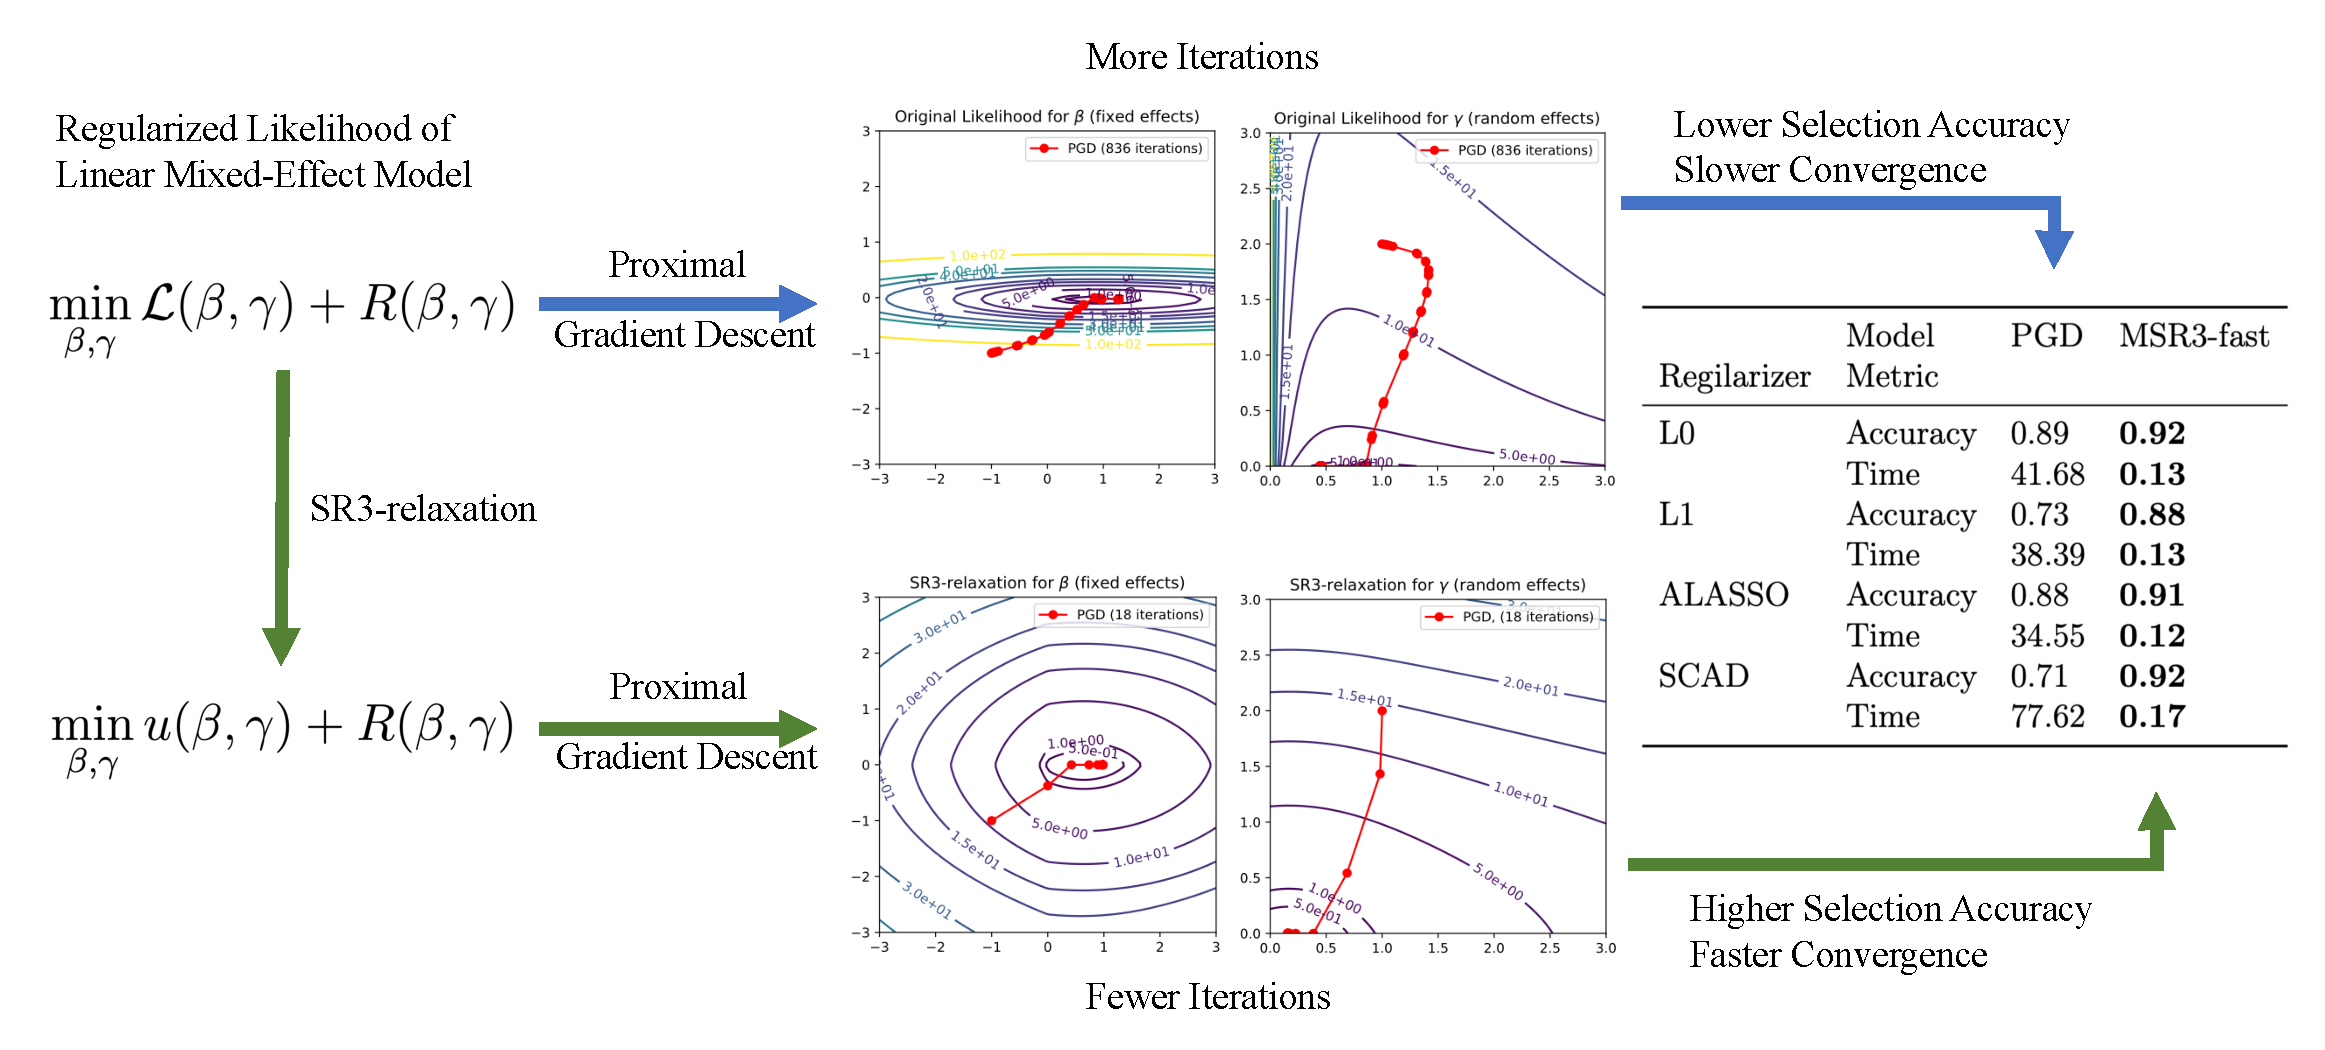
\includegraphics[width=\textwidth]{figures/summary_picture.pdf}
    \caption{Selection of fixed and random effects for LME likelihoods $\mathcal{L}$ using 
    `regularization-agnostic' framework and its SR3 extension using four regularizers. 
    %standard and SR3-relaxed linear mixed-effect likelihoods with popular sparsity-promoting regularizers for the task of simultaneous 
    %The original likelihood $\LL(\beta, \gamma)$ (Eq. \ref{eq:lmm_objective}) is relaxed with SR3 approach to obtain $u(\beta, \gamma)$ (Eq. \ref{eq:value_function_definition}). Both setups are then solved using the same Proximal Gradient Descent (PGD) algorithm. 
    SR3 relaxation accelerates algorithmic converge  (middle panel), and gives better robustness and improved performance on synthetic problems across regularizers (right panel)}.
    \label{fig:summary}
\end{figure}

In this work we introduce a regularization-agnostic covariate selection strategy that (1) is fast and simple to implement, (2) provides robust models, and (3) is flexible enough to support most regularizers currently used in variable selection across different domains.  The baseline approach uses the proximal gradient descent (PGD) method, which has been studied by the optimization community for over 40 years, but has not been widely used in LME covariate selection. 
%We provide proximal operators for commonly used regularizers and show how to apply the PGD method to the nonconvex LME setting. In particular we apply the PGD method to four regularizers, 
%including the $\ell_0$ regularizer, which does not admit local quadratic approximations and has not been used before for LME variable selection strategies. 
In our initial numerical experiments, using a naive PGD approach
indicated that, at best, the method yields only a marginal improvement over the
equally unsatisfactory alternative methods   
in accurately determining the correct variables in our variable selection test problems.
We conjecture that the weakness of the naive PGD is a result of the 
first-order likelihood approximation used in PGD.
To overcome this problem, we propose an alternative likelihood approximation 
with the goal of 
incorporating global variational properties of the likelihood. For this purpose,  
we extend the sparse relaxed regularized regression (SR3) framework~{(\cite{Zheng2019SR3})} to the LME setting. 
This idea is supported
by the success of SR3 in the context of linear regression where it
accelerates and improves the performance of regularization strategies.
This extension and its mathematical foundations in \cite{Theory1} constitute
the major innovations of this work.
Here we introduce the modeling framework and its relaxation, discuss the 
resulting algorithms and their implementation details, and  validate the method on both
simulated and real data sets, while the 
%highly technical 
mathematical 
foundations are presented in \cite{Theory1}.
The SR3 framework introduces auxiliary variables $x$ and $w$ to 
decouple the likelihood $\LL$ and sparsity regularizer $R$ which are tied
together by adding a multiple of the norm squared difference 
$\frac{\eta}{2}\norm{x-w}^2$ to the
objective. 
%We then smooth the positive semi-definite constraint in the 
%likelihood with a log barrier term yielding the smoothed likelihood $\mathcal{L}_\mu$
%where $\mu$ is the smoothing parameter.
Then, fixing the variables $w$ dedicated to the nonsmooth regularizer $R$, 
the smooth function $\LL(x)+\frac{\eta}{2}\norm{x-w}^2$ is
globally optimized over the variables $x$ to obtain an optimal value function
$u_\eta(w)$. We then show that $u_\eta(w)$ is smooth. This opens
the door to the application of the PGD algorithm to minimizing $u_\eta+R$ 
where now $u_\eta$ contains global variational information
on the likelihood function $\LL$. The main obstacle in the
application of this approach is the evaluation of $u_\eta$ and its gradient.
%%%
In Section \ref{sec:MSR3} we present a method for overcoming this difficulty 
using variable metric techniques and interior point technology.
%%%%%%
%To overcome this difficulty we turn to interior point technology. This choice requires 
%smoothing the positive semi-definite constraint on the covariance matrices by
%adding log-barrier term to the likelihood to obtain the smooth function
%$\LL_{\mu,\eta}$ where $\mu$ is the log-barrier relaxation parameter, and
%an associated optimal value function $u_\emu$ whose value and gradients 
%can be quickly and accurately computed.
%%by applying variable metric techniques along with
%%well established properties of the interior point (IP) algorithm to obtain 
%%sufficiently accurate values for
%%both $u_\eta$ and its gradient. 
%Using this underlying framework, we develop two related algorithms,
%MSR3 and MR3-fast where MSR3-fast employs a kind of continuation approach 
%that interlaces approximate IP optimality conditions for the evaluation of 
%$u_\emu$ and its gradient with the prox computation in the PGD algorithm.
%%using a {\it central path} proximity condition from the IP literature.  
%The resulting algorithms are then applied to four regularizers, 
%including the $\ell_0$ regularizer 
%which does not admit local quadratic approximations and 
%has not been used before for LME variable selection strategies.
%The numerical results show that both MSR3 and MR3-fast
%yield superior results over the naive PGD method in terms of specificity and sensitivity of feature selection
%with a slight edge to MR3-fast. However, MR3-fast delivers a spectacular improvement
%in speed over both the naive PGD and the MSR3 algorithms
%(see Table \ref{table:comparison_of_algorithms}).

%We also develop a new meta-approach that can improve the performance of LME selection methods for any regularizer. Specifically, we extend the sparse relaxed regularized regression (SR3) framework~{(\cite{Zheng2019SR3})} to the LME setting. In linear regression, SR3 accelerates and improves the performance of  regularization strategies by introducing auxiliary variables that decouple the accuracy and sparsity requirements for the model coefficients.
%We develop a conceptual and algorithmic approach necessary to extend the SR3 concept to LME.  This development is necessary because the LME problem is nonlinear, nonconvex, and includes constraints on variance parameters.  We show that the new approach yields superior results in terms of specificity and sensitivity of feature selection, and is also computationally efficient.  

All new methods are implemented in an open-source library called \texttt{pysr3}, which fills a gap for python mixed-models selection tools in \texttt{Python} (\cite{Buscemi2019Survey}, Table 3). Our algorithms are  1-2 orders of magnitude faster than available LASSO-based libraries for  mixed effects selection in \texttt{R},  see Table \ref{table:glmmlasso}. \texttt{pysr3} enables a standardized comparison of different methods in the LME setting, and makes both the PGD framework and its SR3 extension available to practitioners working with LME models. 
%\subsection{Notation}
%\begin{enumerate}
%\item sets like $\N$, $\B$, $\bS$, $\SS$.
%\item nonsmooth stuff, subdifferential and normal cones
%\end{enumerate}

%Roadmap
We begin in Section \ref{sec:LMEM} by giving a precise description of the LME
model and set the notation for the remainder of the section. 
This is followed by a brief discussion of prior work on LMEs.
In Section \ref{sec:pgd_methods} we present our algorithms for the LME model 
starting with the naive PGD algorithm. This is followed by a description of the 
variable splitting technique used in \cite{Zheng2019SR3} to incorporate global 
variation information on the likelihood function into the direction finding subproblem
for the PGD algorithm. 
%This lays the foundation for the MSR3 algorithm. 
Next we tackle the problem of how to approximate the 
resulting optimal value function $u_\eta$ and its gradient where $\eta>0$ is the 
decoupling parameter. As noted, this is done using variable metric techniques and 
and interior point technology. We conclude Section \ref{sec:pgd_methods} 
with a discussion of the
MSR3 and MSR3-fast algorithms. In Section \ref{sec:applications} we discuss how
the underlying algorithmic parameters are set and test the algorithm on both 
simulated problems and a problem with real data. In Section~\ref{sec:theory-paper} we develop theoretical underpinnings of the proposed extension, including consistency results, variational properties, implementability of optimization methods, and convergence results for both MSR3 and MSR3-fast. Section~\ref{sec:software-paper} outlines the software implementation of MSR3 and MSR3-fast in \texttt{pysr3} package. The chapter is concluded in Section \ref{sec:discussion} with a brief discussion of the contributions.

\section{Linear Mixed-Effects Models: Notation and Fundamentals}\label{sec:LMEM}
Mixed-effect models describe the relationship between an outcome variable and its predictors when the observations are grouped, for example in studies or clusters.  To set the notation, consider $m$ groups of observations indexed by $i$, with sizes $n_i$, and the total number of observations equal to $n = n_1 + n_2 + \dots + n_m$. For each group, we have design matrices for fixed features $X_i \in \R^{n_i \times p}$,  and matrices of random features $Z_i \in \R^{n_i \times q}$, along with vectors of outcomes $Y_i \in \R^{n_i}$. 
%Typically, columns of $Z_i$ are a subset of columns $X_i$ but it does not have to be the case in general. 
Let 
{$X = [X_1^T, X_2^T, \dots, X_m^T]^T$ and $Z = [Z_1^T, Z_2^T, \dots, Z_m^T]^T$.} 
Following~\cite{Patterson1971, Pinheiro2000}, we define a Linear Mixed-Effects (LME) model as
\begin{equation}
\begin{aligned}
	Y_i & = X_i\beta + Z_iu_i + \varepsilon_i, \quad i = 1 \dots m \\
	u_i & \sim \NN(0, \Gamma),\quad \Gamma \in \bS_{+}^{q} \\
	\varepsilon_i & \sim \NN(0, \Lambda_i), \quad \Lambda_i \in \bS_{++}^{n_i}
	\end{aligned}
	\label{eq:lme_setup}
\end{equation}
 where $\beta \in \R^p$ is a vector of fixed (mean) covariates, 
 $u_i \in \R^{q}$ are unobservable random effects assumed to be distributed normally with zero mean and the unknown covariance matrix $\Gamma$, and $\bS_{+}^{\nu}$ 
 and $\bS_{++}^{\nu}$ are the sets of
 real symmetric $\nu\times \nu$ positive semi-definite
 and positive definite matrices, respectively. 
Matrices $Z_i$ encode a wide variety of models, including
random intercepts ($Z_i$ are columns of 1's that add $u_i$ to all datapoints from the $i$th study)
and random slopes ($Z_i$ also scale $u_i$ according to the magnitude of a covariate), see e.g.~\cite{pinheiro2006mixed}. 
%In these typical examples, the columns of $Z_i$ are subsets of the columns
%of $X_i$.  
In our study, we assume that the observation error covariance matrices 
$\Lambda_i$ are given and that the random effects covariance matrix 
is an unknown diagonal matrix, i.e., $\Gamma = \Diag{\gamma}, \ \gamma \in \R^s_+$.
This assumption corresponds to the meta-analysis and meta-regression branch of mixed effects problems, 
which is the primary focus of our applied collaborations~ (see e.g. \cite{zheng2022burden,lescinsky2022health,razo2022effects,stanaway2022health,dai2022health}.)
The theoretical developments in this work allow extensions to other types of repeated measure models, 
but practical implementation requires significant additional effort, and we leave these extensions to future work.  

% either
% assumed to have a simple parametric form, such as $\Lambda_i=\sig_i I$
% with $\sig_i$ to be determiined, or given given  
 %; we focus on the latter case below. 
 
Defining group-specific error terms $\omega_i = Z_i u_i + \varepsilon_i$, we get a compact formulation that 
recasts~(\ref{eq:lme_setup}) as a correlated noise model:
 \eq{
 \label{eq:lmm_correlated_noise_setup}
	Y_i = X_i\beta + \omega_i,\quad \omega_i \sim \NN(0, \Omega_i(\Gamma)), \quad \Omega_i(\Gamma) = Z_i\Gamma Z_i^T + \Lambda_i.
}
For brevity, we refer to $\Omega_i(\Gamma)$ as just $\Omega_i$.
%without the parentheses. In fact, $\Omega_i$ will be the only terms depending on $\Gamma$ in the majority of expressions including the mixed model's likelihood and its derivatives described below.
The reformulation \eqref{eq:lmm_correlated_noise_setup}
yields the following marginalized  negative log-likelihood function of a linear mixed-effects model~\citep{Patterson1971}:
\eq{
	\label{eq:lmm_objective}
	\LL_{ML}(\beta, \Gamma)  :=
%	 \textabove{$\Delta$}{=}
	 \sum_{i = 1}^m \half(y_i - X_i\beta)^T\Omega_i^{-1}(y_i - X_i\beta) + \half\ln{\det{\Omega_i}}.
}
Maximum likelihood estimates for $\beta$ and $\Gam$ are obtained by
solving the optimization problem
\eq{
	\label{eq:ml_lme_optimization_setup}
	\min_{\beta, \Gamma} & \ \LL_{ML}(\beta, \Gamma)  \quad \mbox{s.t.} \quad \ \Gamma \in \bS_{+}^{q}.
}

\begin{theorem}[Existence of a Minimizer, Theorem 1 from \cite{aravkin2022jimtheory}]\label{thm:basic existence}
Let the assumptions in the statement of problem \eqref{eq:ml_lme_optimization_setup} hold. Then optimal solutions to
\eqref{eq:ml_lme_optimization_setup} exist.
\end{theorem}

At this point, we bring in three basic definitions from variational analysis~\cite{rockafellar2009variational}. 

\begin{definition}[Epigraph and level sets]
The epigraph of a function $f:\mathbb{R}^n\rightarrow \mathbb{R} \cup \{\infty\}$ is defined as
\[
\epi f = \{(x,\alpha) : f(x) \leq \alpha\}. 
\]
For a given $\alpha$, the $\alpha$-level set of $f$ is defined as
\[
\text{lev}_\alpha f = \{x: f(x) \leq \alpha\}.
\] 
\end{definition}

\begin{definition}[Lower semicontinuity and level-boundedness]
A function $f:\mathbb{R}^n\rightarrow \mathbb{R} \cup \{\infty\}$ is lower semicontinous (lsc) when $\epi f$ is closed, 
and level-bounded when all level sets $\text{lev}_\alpha f$ are bounded.  
\end{definition}

\begin{definition}[Convexity]
A function $f:\mathbb{R}^n\rightarrow \mathbb{R} \cup \{\infty\}$ is convex when $\epi f$ is a convex set. Equivalently, 
\[
f(\lambda x + (1-\lambda)y) \leq \lambda f(x) + (1-\lambda) f(y) \quad \forall x,y\in\dom{f},\ \lambda \in (0,1),
\]
where $\dom{f}:=\lset{x\in\Rn}{f(x)<+\infty}$.
\end{definition}

\begin{definition}[Weak convexity]
A function $f:\mathbb{R}^n\rightarrow \mathbb{R} \cup \{\infty\}$ is $\eta$-weakly convex 
$f(\cdot)+\frac{\eta}{2}\|\cdot\|^2$ is convex. 
\end{definition}

The negative log likelihood~\eqref{eq:ml_lme_optimization_setup}  is nonlinear and nonconvex, and requires an iterative numerical solver.
However, it is convex with respect to $\beta$, and weakly convex with respect to $\gamma$, with a weak convexity constant $\overline \eta$
computed in~\cite[Section 5.1]{Theory1} . The expected value of the posterior mode $\beta$ given $\Gamma$ has the closed form representation 
	
\begin{equation}
	\label{eq:beta_formula}
	\beta(\Gamma) = \argmin_{\beta}\LL(\beta, \Gamma) = \left(\sum_{i = 1}^m X_i^T\Omega_i^{-1}X_i\right)^{-1}\sum_{i = 1}^mX_i^T\Omega_i^{-1}y_i.
\end{equation}

The individual random effects $u_i$ can be found through the minimization of conditional likelihood of random effects given $\beta$ and $\Gamma$:

\eq{
\min_{u_i}\LL(u_i|\beta, \Gamma) = \min_{u_i}\left(\half u_i^T\Gamma^{-1}u_i + \half (Z_iu_i - Y_i + F_i(\beta))^T\Lambda_i^{-1}(Z_iu_i - Y_i + F_i(\beta))\right),
}

This problem has a closed form solution commonly known as Best Linear Unbiased Predictor, or BLUP. It was first derived by \cite{Harville1976} as an extension to Gauss-Markov theorem.

 \eq{
	\label{eq:random_effects_formula}
	u_i = (\Gamma^{-1} + Z_i^T\Lambda_i^{-1}Z_i)^{-1}Z_i^T\Lambda_i^{-1}(Y_i - X_i\beta).	
}


By using the simplification $\Gam=\Diag{\gam}$, we obtain the problem
%{In the meta-analysis setting under study, 
%In our study, we assume that $\Gam$ is a diagonal matrix of the form
%$\Gamma = \Diag{\gamma}, \ \gamma \in \R^s$ with the 
%$\Lambda_i \in \R_{++}^{n_i \times n_i}$ fixed and given 
%%the positive definite constraint from (\ref{eq:ml_lme_optimization_setup}) transforms into a box constraint:
%so that our problem takes the form}
\eq{
	\label{eq:lme_diagonal_setup}
	\min_{\beta\in\R^p, \gam\in\R^q_+} & \ \LL(\beta,\gam)
	:=\LL_{ML}(\beta, \Diag{\gamma}) \, .
%	\\
%	s.t. & \ \gamma \geq 0\ .
	}
%Under the assumption $\Lambda_i \in \R_{++}^{n_i \times n_i}$ in~\eqref{eq:lme_setup}, 
In this setting, when an
entry $\gamma_j$ takes the  value $0$ the corresponding coordinates of all random effects $u_{ij}$ are identically $0$ for all $i$. 

Verification of the existence to solutions to \eqref{eq:lme_diagonal_setup}
and, more generally, \eqref{eq:ml_lme_optimization_setup} follows from the work of \cite{zheng2021trimmed}.
Standalone proofs for the existence of minimizers are developed in~\cite[Theorem 1]{Theory1},
and extended to the presence of regularizers in~\cite[Theorem 2]{Theory1}. %, restated below for convenience. 


%%Here we streamline these techniques and extend to the regularized case, 
%%with basic results given below, with proofs in the appendix.  
%
%\begin{theorem}[Existence of a Minimizer]\label{thm:basic existence}
%Let the assumptions in the statement of problem \eqref{eq:ml_lme_optimization_setup} hold. Then optimal solutions to
%\eqref{eq:ml_lme_optimization_setup} exist.
%\end{theorem}
%
%Feature selection methods  include sparsity-inducing penalties or constraints. See~\cite[Theorem 1]{Theory1}
%for an existence result under weak assumptions on the regularizer. 
%
%
% 
%
%\begin{theorem}\label{thm:basic existence2}
%Let the assumptions in the statement of problem \eqref{eq:lme_diagonal_setup} hold,
%define $\LL(\beta,\gam):=\LL_{ML}(\beta, \Diag{\gamma})$
%and suppose $\map{\hR}{\R^p\times\R^q_+}{\R\cup\{+\infty\}}$ 
%is lsc and level bounded.
%Then $\LL+\hR$ is level bounded and solutions to
%the following optimization problem exist:
%\eq{
%\label{eq:extended loss}
%\min_{\beta\in\R^p, \gamma\in\R^q_+}  \LL(\beta, \gamma) + 
%\hR(\beta, \gamma) .
%}
%\end{theorem}

%\red{I don't get the point of the following paragraph. Indeed, it seems wrong.}

Our work focuses the case where $\Gamma$ is diagonal, 
  (often referred to as \textit{the diagonal setup}) 
 and all $\Lambda_i$ are known (see \eqref{eq:lme_diagonal_setup}), 
following the meta-analysis use-case~\citep{zheng2021trimmed} that is widely 
employed in epidemiological studies~\cite{murray2020global}. 
While the proposed approach can be extended to the non-diagonal case, we leave it for future work, save for a brief discussion in Section~\ref{sec:applications}.

\subsection{Prior Work on Feature Selection for Mixed-Effects Models}
\label{sec:prior_work}

Variable (feature) selection models seeks to select or rank the most important predictors in a dataset in order to get a parsimonious model at a minimal cost to prediction quality. 
Feature selection may be performed both on $\beta$, to find the sparse set of covariates that best explains the mean, and on $\gamma$, to find the sparse set of covariates that best accounts for 
variation between groups. Both types of selection have been studied in the literature, and both are accessible using the methods developed here.
%The selection process often occurs simultaneously with fitting the model, and a predictor is `selected' if its respective coefficient in the model is non-zero. 
If the desired number of coefficients $k$ is given, then the feature selection problem can be formulated as the minimization of a loss function $f(\theta)$ (e.g. the negative log-likelihood) subject to a zero-norm constraint:
\eq{
	\label{eq:general_feature_selection_zero_norm}
	&\min_{\theta}  f(\theta) \quad \mbox{ s.t. }  \quad \|\theta\|_0 \leq k 
	}
where $\|\theta\|_0$ denotes the number of nonzero entries in $\theta$, see panel (c) of Figure~\ref{fig:regularizers}.

%\begin{figure}
%    \centering
%    \begin{tabular}{cc}
%    \includegraphics[width=0.3\textwidth]{figs/l0_regularizer.pdf}
%    &
%        \includegraphics[width=0.3\textwidth]{figs/l1_regularizer.pdf}\\
%        (a) $\ell_0$ & (b) $\ell_1$ \\
%           \includegraphics[width=0.3\textwidth]{figs/lh_regularizer.pdf}
%    &
%        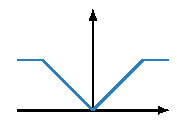
\includegraphics[width=0.3\textwidth]{figs/scad_regularizer.pdf}\\
%              (a) $\ell_{1/2}$ & (b) Clipped Absolute Deviation (CAD) 
%    \end{tabular}
%    \caption{Common convex and non-convex regularizers used for feature selection.}
%    \label{fig:regularizers}
%\end{figure}


% In this form the problem is equivalent to the Knapsack problem, which is NP-complete. Many techniques based on exhaustive search, also known as subset selection process, were developed, and showed to be effective when the total number of predictors is small (see \cite{Muller2013}). The same setup appears to be intractable in a high-dimension setting due to the exponential growth of the number of subsets to check when $n \to \infty$, however, it's possible to get an approximate solution via relaxation techniques.

 \begin{figure}[ht!]
    \centering
    \begin{tabular}{ccc}
        \includegraphics[width=0.3\textwidth]{figures/l1_regularizer.pdf}
&
           \includegraphics[width=0.3\textwidth]{figures/lh_regularizer.pdf}
    &
    \includegraphics[width=0.3\textwidth]{figures/l0_regularizer.pdf}\\
  %      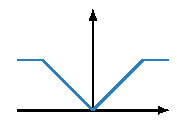
\includegraphics[width=0.3\textwidth]{figs/scad_regularizer.pdf}\\
              (a) $\ell_1$  & (b) $\ell_{1/2}$ & (c) $\ell_0$
    \end{tabular}
    \caption{Common convex and non-convex regularizers used for feature selection.}
    \label{fig:regularizers}
\end{figure}


The constraint in \eqref{eq:general_feature_selection_zero_norm} is 
combinatorial, and a common workaround is to relax it to a one-norm constraint, 
with $\|\theta\|_1$ equal to the sum of absolute values of the entries of $\theta$. 
The best-known example of this approach is the least absolute square shrinkage operator (LASSO) studied by \cite{Tibshirani1996} for linear regression, 
see panel (a) of Figure~\ref{fig:regularizers}.
% for the least squares model:
% \eq{
% 	\label{eq:lasso_regression}
% 	\min_\theta f(\theta) + \lambda||\theta||_1
 %
 
% LASSO combines the small bias of the least-square estimator and the interpretability of the subset selection method, producing
% %, however, 
% biased estimates for the large coefficients~\citep{Zou2006}.  This approach has been extended to leverage many other regularizers that exhibit useful properties including bias 
%reduction for larger coefficients (SCAD from \cite{Fan2001}), simultaneous selection for highly correlated predictors (Elastic Net from \cite{Zou2005}), or better selection accuracy using non-penalized solution's coordinates as weights (A-LASSO from \cite{Zou2006}).
  
 Feature selection for LMEs is more difficult than for linear regression models. 
 In linear regression the observations are independent, whereas in mixed-effects setup they are generally correlated. 
 In addition, LMEs have both mean effect variables  $\beta$ as well as random variance variables 
 $\Gamma$. % where the groups can have different relative importance. 
% Finally, selecting random features implies that $\Gamma$ will have zero columns and rows thereby forcing the optimization methods to the boundary of the feasible parameter set and making both the theoretical analysis and numerical computations more challenging.  
The shrinkage operator approach for linear regression 
\citep{Tibshirani1996} was first adapted 
to the problem of feature selection for the fixed effects in mixed-effect models by \cite{Lan2006}. 
The removal of a random effect from the model requires the elimination of an entire row and column from $\Gamma$. 
To make the problem more tractable, \cite{Chen2003} reparamtrized $\Gamma$ through a modified Cholesky decomposition $\Gamma(D,L): = DLL^TD$, where $D$ is a diagonal matrix and $L$ is a lower-triangular matrix with ones on the main diagonal, and focused on selecting elements of $D$. 
% In this case, one can select variance parameters by selecting the elements of the diagonal matrix $D$ while treating the non-diagonal entries of $L$ as free parameters. 
Based on this idea, \cite{Krishna2008} extended the Adaptive LASSO regularizer (\cite{Lan2006, Xu2015}) to mixed-effects setting using the objective
   \(
        \LL(\beta, \Gamma(D,L)) + \lambda\left(\sum_{i = 1}^p 
        \left|\frac{\beta_i}{\hat\beta_i}\right| + \sum_{j = 1}^q \frac{D_{ii}}{\hat{D_{ii}}} \right),
   \)
 where $\hat\beta$ and $\hat{D}$ are the solution of a non-penalized maximum likelihood problem and $\lambda$ is a tuning parameter for the weighted regularizer
 and is called the regularization parameter. 
 %This strategy has a well known issue: non-penalized estimates $\hat\beta$ and $\hat{D}$ may be inaccessible because the numerical algorithm may fail to converge, especially when the underlying solution is sparse. 
 \cite{Ibrahim2011} use a similar approach, penalizing  non-zero elements $\Gamma_{ij}$ directly. 
 Other methods that use Adaptive LASSO for simultaneous selection 
 of fixed and random effects are \cite{Lin2013, fan2014robust, pan2018simultaneous}. Adaptive LASSO is available to practitioners via \texttt{R} packages \texttt{glmmLasso}\footnote{\href{https://rdrr.io/cran/glmmLasso/man/glmmLasso.html}{https://rdrr.io/cran/glmmLasso/man/glmmLasso.html}} (\cite{groll2014variable}) and \texttt{lmmLasso}\footnote{\href{https://rdrr.io/cran/lmmlasso/}{https://rdrr.io/cran/lmmlasso/}}(\cite{schelldorfer2011estimation}).

 A popular nonconvex regularizer used for feature selection is smoothed clipped absolute deviation (SCAD)~\cite{Fan2001}. 
 %The (non-smoothed) clipped absolute deviation penalty is depicted in panel (d) of Figure~\ref{fig:regularizers}.
% , and the algebraic forms for both CAD and SCAD are given in the appendix. 
% which acts on the first derivative of the penalty function $p_\lambda(\theta)$:
 %  \eq{
  % 		p'_{\lambda}(|\theta|) = \lambda\left\{\ind{\theta \leq \lambda} +  \frac{(a\lambda - \theta)_+}{(a-1)\lambda}\ind{\theta - \lambda} \right\}
  % }
The adaptation of the SCAD penalty to select both fixed and random features in 
linear mixed models was developed by \cite{Fan2012}. SCAD was also used by \cite{chen2015inference} for selecting fixed effects and establishing the existence of random effects in ANOVA-type models. Finally, \cite{Ghosh2018} studied SCAD regularization for selecting mean effects in high-dimensional genomics problems. One can refer to \cite{Muller2013, Buscemi2019Survey} for a detailed overview of different feature selection approaches.

To better compare methods, we need to consider the tuning of the regularization parameter 
$\lambda$. 
The output of a shrinkage model critically depends on the tuning parameter 
$\lambda$. The entire range of $\lambda$ values is captured 
by the notion of a ``$\lambda$-path in the model space'', with  the best parameter and the final model chosen using information criteria. According to \cite{Muller2013}, the most widely used information criterion is the marginal AIC criterion (\cite{Vaida2005}),
 \(  AIC := 2\LL(\hat{\theta}) + 2\alpha_n(p+q)\), 
  where $\hat\theta$ includes all the estimated parameters $(\beta, \Gamma)$, and $\alpha_n := n(n-p-q-1)$ for the finite sample case (\cite{Sugiura1978}). 
  %As discussed by \cite{Fang2011}, AIC is asymptotically equivalent to leave-one-out cross-validation, so it can be used for choosing between a finite number of models. AIC, however, is also known to be positively-biased (\cite{Ibrahim2011}). 
  Alternatively, LASSO-type methods (\cite{Krishna2008, Ibrahim2011}) use a BIC-type information criterion,  \(BIC := 2\LL(\hat{\theta}) + \log(n)(p+q)\).
BIC performs well in practice, but does not have theoretical guarantees~(\cite{schelldorfer2011estimation}). Finally, \cite{Hui2017} suggests penalizing the number of non-zero random effects in the resulting model instead of penalizing the number of random features with non-zero variance, especially when random effects are optimized directly instead of using BLUP~\eqref{eq:random_effects_formula}.
  
\section{Algorithms for Feature Selection}
\label{sec:pgd_methods}
We approach feature selection by adding a regularizer to model \eqref{eq:lme_diagonal_setup}: 
%( $\Lam_i$ are known and given, and $\Gamma$ an unknown diagonal matrix,   
%to be estimated along with the fixed effects $\beta$. 
%and add a regularizer:
%to the objective to obtain the optimization problem described
%in Theorem \ref{thm:basic existence2}:

%Feature selection is imposed by adding
%Consider a mixed-effect model setting described in Eq. (\ref{eq:lme_setup}) with $\Gamma$ being diagonal: $\Gamma = \Diag{\gamma}$.  
%We wish to find a minimizer of the problem 
%\eq{
%	\label{eq:lme_loss_original}
%	\min_{\beta\in\R^p, \gamma\in\R^q_+} & \LL(\beta, \gamma) + R(\beta, \gamma), 
%	}
%\vskip -.5in
\eq{%\label{eq:main opt in x over C}
     \min_{x } & \LL(x) + R(x)+ \delta_{\CC}(x),
      \label{eq:lme_loss_original_in_x}
%    \\
%    \text{s.t. } & x \in \CC\ .
}
where $x = (\beta, \gamma)$, 
$\CC:=\R^p\times \R^q_+$,
$\map{R}{\R^P\times\R^q_+}{\eR_+:=\R_+\cup\{+\infty\}}$
is a 
lower semi-continuous (lsc) regularization term, and
$\delta_{\CC}$ is the convex indicator function, where
$\delta_{\CC}(x) :=0$ for $x \in \CC$ and $+\infty$ otherwise.
%\[
%    \delta_{\CC}(x) := \begin{cases} 0, &  x \in \CC \\ +\infty, & x \not\in \CC .\end{cases}
%\]  
By \cite[Theorem 2]{Theory1}, solutions to \eqref{eq:lme_loss_original_in_x}
always exist when $R$ has compact lower level sets.
% or 
% $\LL(\beta, \gamma)=\LL_{REML}(\beta,\Diag(\gamma))$ in \eqref{eq:reml_objective} with 
% \[
% \B=[\zero,\gam_\mmax\one]:=\left\{ \gamma\, |\, 0\le \gamma_i\le \gam_\mmax,\ i=1,\dots,q\right\}
% \]
% for some $\gam_\mmax>0$ where $\one$ is the vector of the appropriate
% dimension each of whose components is one.
% Since the method applies to either likelihood, hereafter we omit the subscripts and use $\LL$ to denote the objective function. %, leaving this choice up to a practitioner.
%For conciseness, define $x = (\beta, \gamma)$ and 
%$\CC:=\R^p\times \R^q_+$.
%such that $\tbeta \in \R^p$ is unconstrained and $\tgamma \in \R^q_+$ is non-negative:
%\eq{
% x\in \CC \textabove{$\Delta$}{=} \{[\beta', \gamma']: \  \beta' \in \R^p, \ \gamma' \in \R^q_+\} \subset \R^{p+q} 
%}
%With this notation, problem \eqref{eq:lme_loss_original} becomes
%\eq{%\label{eq:main opt in x over C}
%    \label{eq:lme_loss_original_in_x}
%    \min_{x \in \CC} & \LL(x) + R(x),
%    \\
%    \text{s.t. } & x \in \CC\ .
%}
%Equivalently, the box constraint can be moved to the loss in a form of an indicator function:
%or equivalently
%\[
%\eq{
%	\label{eq:lme_loss_original}
%    \min_{x} \LL(x) + R(x) + \delta_{\CC}(x)\ ,
%}
%where 
%$x = (\beta, \gamma)$, 
%$\CC:=\R^p\times \R^q_+$,  
%\quad \text{where}\ \, 
%\delta_{\CC}$ is the convex indicator function
%\[
%    \delta_{\CC}(x) := \begin{cases} 0, &  x \in \CC \\ +\infty, & x \not\in \CC .\end{cases}
%\]
The most common regularizers are separable taking the form
\begin{equation}\label{eq:R sep}
R(x) = \sum_{i = 1}^p r_i(x_i), 
\end{equation}
with typical choices for the component functions $r_i$ given in Table \ref{table:proxes}.




\subsection{Variable Selection via Proximal Gradient Descent}

Since $\LL$ is differentiable on its domain and 
proximal operator
for $\alpha R + \delta_{\CC}$ is 
computationally tractable, 
the Proximal Gradient Descent (PGD) Algorithm (e.g. see \cite{AB17}) offers a simple numerical
strategy for estimating first-order stationary points for 
\eqref{eq:lme_loss_original_in_x}.
% when 
%the application of the . 
%
%whenever the application of the proximal operator \cite{}
%to $\alpha R + \delta_{\CC}$ is 
%computationally tractable, a simple numerical method for estimating
%first-order stationary points for \eqref{eq:lme_loss_original_in_x} is
%the Proximal Gradient Descent (PGD) Algorithm. 
The proximal operator for 
$\alpha R + \delta_{\CC}$ is defined as the mapping
\( %\eq{
    \prox_{\alpha R + \delta_{\CC}}(z) := \argmin_{y\in \CC}\ R(y) + \frac{1}{2\alpha}\|y - z\|_2^2 ,
\) %}
and the PGD iteration is given by
\(
    x^+ = \prox_{\alpha R + \delta_{\CC}}(x - \alpha \nabla \LL(x)),
\)
where $\alpha$ is a stepsize.
When $R(x)$ has the form given in \eqref{eq:R sep}, we have
\(
 \prox_{R}(z) = (\prox_r(z_1), \dots, \prox_r(z_q)) .
\)
Table \ref{table:proxes} provides closed form expressions for the proximal operators 
of commonly used regularizers. 
For all of these cases,  the following theorem gives closed form expressions for
$\prox_{\alpha R + \delta_{\CC}}(z)$.


\begin{table}[H]
\small
    \centering
    \begin{tabular}{|p{25.4mm}|c|c|}
        \hline
         \!\!Regularizer & $r(x)$, $x \in \R$ & $\prox_{\alpha r}(z)  $ \\
         \hline \hline
         LASSO ($\ell_1$) \newline & $|x|$ & $\sign(z)(|z| - \alpha)_+$ \\
         \hline
         A-LASSO \newline  & $\bar{w}|x|$, $\bar{w} \geq 0$ &  $\sign(z)(|z| - \alpha\bar{w})_+$\\
         \hline
         SCAD \newline & $\begin{cases} \sigma |x|, & |x| \leq \sigma \\ \frac{-x^2 + 2\rho\sigma x - \sigma^2}{2(\rho - 1)}, & \sigma < |x| < \rho\sigma \\ \frac{\sigma^2(\rho + 1)}{2}, & |x| > \rho\sigma \end{cases}$ & $\begin{cases} \sign(z)(|z| - \sigma\alpha)_+, & |z| \leq \sigma(1+\alpha) \\ \frac{(\rho - 1)z - \sign(z)\rho \sigma\alpha}{\rho - 1 - \alpha}, & \sigma(1+\alpha) < |z| \leq \rho\sigma
         %\max(\rho, 1+\alpha)\sigma 
         \\ z, & |z| > \max(\rho,1+\alpha)\sigma \end{cases}$ \\
%         \hline
%         $\ell_p$, $0 < p < 1$ & $|x|^p$ & Coordinate Newton (\cite{Zheng2019SR3}) \\
         \hline
         $\delta_{\|x\|_0 \leq k}$  \newline ($\ell_0$ ball) & $\begin{cases} 0, & \#\{|x_i| \neq 0\} \leq k\\ \infty, & \text{ otherwise}\end{cases}$ & keep $k$ largest $|x_i|$, set the rest to 0 \\
         \hline
    \end{tabular}
    \caption{Proximal operators for commonly used sparsity-promoting regularizers. }
    \label{table:proxes}
\end{table}

Under the assumption that $R$ is level-compact \cite{aravkin2022jimtheory} extended Theorem \ref{thm:basic existence} to the regularized case as follows:

\begin{theorem}[Existence of a Minimizer for \ref{eq:lme_loss_original_in_x}, \cite{aravkin2022jimtheory}, Theorem 2]

\label{thm:basic existence2}
Let the assumptions in the statement of problem \eqref{eq:lme_diagonal_setup} hold.
%define $\LL(\beta,\gam):=\LL_{ML}(\beta, \Diag{\gamma})$
Suppose $\map{\hR}{\R^p\times\R^q_+}{\R\cup\{+\infty\}}$ 
is lsc and level compact (i.e., $\epi{R}:=\lset{(\bg,\nu)}{R\bg\le\nu}$ is closed
and $\lset{\bg}{R\bg\le\nu}$ is bounded for all $\nu\in\R$).
Then $\LL+\hR$ is level compact and solutions to
the following optimization problem exist:
\eq{
\label{eq:extended loss}
\min_{\beta\in\R^p, \gamma\in\R^q_+}  \LL(\beta, \gamma) + 
\hR(\beta, \gamma) .
}
\end{theorem}

In practice, it is often advisable to include a constraint of the form 
$\gamma\le\gammax$ for $\gam\in\R^q_{++}$ chosen
sufficiently large since an excessively large variance usually indicates 
that the model is poorly posed and needs review. 
Such a constraint is also numerically expedient since it prevents $\gam$ from diverging. Table \ref{table:proxes} provides closed form expressions for the proximal operators 
of commonly used regularizers. 

%All regularizers in this list are separable except $R(x) = \delta_{\|x\|_0 \leq k}$, for which the solution also has an analytically closed form.
%Again when $R$ is separable with the $r_i$ coming from Table \ref{table:proxes}, 
%the evaluation of 

\begin{theorem}[Proximal operator for bounded $\gamma$]     \label{thm:prox_of_positive_quadrant}
We consider modified regularizers $r(\gamma)$ from the Table \ref{table:proxes} 
% and let $v = (\beta, \gamma)$. % \in \CC \subset R^{p + q}$.
that include an additional constraint on $\gamma$ of the form 
\(
0 \leq \gamma \leq \bar\gamma,
\)
for $\bar\gamma\in[0,+\infty]$.
%which which the positive orthant as a special case (i.e. $\bar\gamma = \infty$). 
We have the following results. 
%    \begin{enumerate}
%    \item  For $R(x)$ given by LASSO, A-LASSO, CAD, and SCAD, we have  for all $i$ that 
    %\eq{
    %\prox_{\alpha R + \delta_{\CC}}(v) = (\prox_{\alpha r}(v_1), \dots, \prox_{\alpha r}(v_p), \prox_{\alpha r + \delta_{\R_+}}(v_{p+1}), \dots, \prox_{\alpha r + \delta_{\R_+}}(v_{p+q}))
    %}
    %where 
 %   \eq{
 %   \prox_{\alpha r + \delta_{\R_+}}(v_{i}) = \begin{cases} \prox_{\alpha r}(v_i), & v_i \geq 0 \\ 0, & \text{ otherwise} \end{cases} 
%    \item For $R(x) = \delta_{\|x\|_0 \leq k}$, the $\prox_{\alpha R + \delta_{\CC}}(v)$ can be evaluated by taking $k$ largest non-negative coordinates of $v$, and setting the rest to $0$.
 %   \end{enumerate}
%    Next, suppose $\LL = \LL_{REML}$. 
    \begin{enumerate}
    \item  For SCAD, we have for all $i$ that \;
   % \eq{
%    \prox_{\alpha R + \delta_{\CC}}(v) = (\prox_{\alpha r}(v_1), \dots, \prox_{\alpha r}(v_p), \prox_{\alpha r + \delta_{\R_+} + \delta_{\R_{\leq \bar\gamma}}}(v_{p+1}), \dots, \prox_{\alpha r + \delta_{\R_+} + \delta_{\R_{\leq \bar\gamma}}}(v_{p+q}))
 %   }
  %  where 
%    \eq{
\(
    \prox_{(\alpha r + \del_{[0,\bgam]})} %\delta_{\R_+} + \delta_{\R_{\leq \bar\gamma}}}
    (\gamma_{i}) = \begin{cases} 
        \prox_{\alpha r}(\gamma_i), & 0 \leq \gamma_i < \bar\gamma  \\
        \bar\gamma, & \gamma_i \geq \bar\gamma \\
        0, & \text{ otherwise} \end{cases}.
\)
%    }
    \item  For LASSO, A-LASSO we have for all $i$ that \;
 %   \eq{
  %  \prox_{\alpha R + \delta_{\CC}}(v) = (\prox_{\alpha r}(v_1), \dots, \prox_{\alpha r}(v_p), \prox_{\alpha r + \delta_{\R_+} + \delta_{\R_{\leq \bar\gamma}}}(v_{p+1}), \dots, \prox_{\alpha r + \delta_{\R_+} + \delta_{\R_{\leq \bar\gamma}}}(v_{p+q}))
  %  }
  %  where 
%    \eq{
\(
\prox_{(\alpha r + \del_{[0,\bgam]})}(\gamma_i) 
%    \prox_{\alpha r + \delta_{\R_+} + \delta_{\R_{\leq \bar\gamma}}}(v_{i}) 
    = \begin{cases} 
        \prox_{\alpha r}(\gamma_i), & 0 \leq \gamma_i < \bar\gamma + \alpha \\
        \bar\gamma, & \gamma_i \geq \bar\gamma + \alpha \\
        0, & \text{ otherwise} \end{cases}.
\)
%    }
    \item For $R(\cdot) = \delta_{\lev{\norm{\cdot}_0}{k}}$  %\delta_{\|x\|_0 \leq k}$, 
    the $\prox_{\alpha R + \delta_{\CC}}(\gamma)$ can be evaluated by taking $k$ largest coordinates of $\gamma$ such that $0 \leq \gamma_i \leq \bar\gamma$, and setting the 
    remainder to $0$.
    \end{enumerate}
\end{theorem}
The proof of the Theorem \ref{thm:prox_of_positive_quadrant} is provided in Appendix \ref{appendix:proxes}. 
%\textcolor{red}{Aleksei, please check proof of appendix is all in terms of $\gamma$, rather than $v = (\beta, \gamma)$.}
The  PGD algorithm is detailed in Algorithm~\ref{alg:pgd_for_lme}.
{The algorithm's step-size $\alpha$ depends on the Lipschitz constant; an upper-bound is given in Appendix \ref{appendix:lipschitz_constant}. In practice, $\alpha$ is computed using a line-search, since the available estimate for $L$ is very conservative.}

\smallskip

\begin{algorithm}[H]
\SetAlgoLined
$x = x_0$, $\alpha < \frac{1}{L}$,\text{ where } $\LL$ \text{ is $L$-Lipschitz}\\
 \While{not converged}{
    $x^+ = \prox_{\alpha R + \delta_{\CC}}(x - \alpha \nabla \LL(x))$;\\
 }
 \caption{\label{alg:pgd_for_lme}Proximal Gradient Descent for Linear Mixed-Effect Models}
\end{algorithm}
\medskip

\noindent

The main advantages of Algorithm \ref{alg:pgd_for_lme} are its simplicity and flexibility.
The main loop needs only the gradient and prox operator, and the structure of the algorithm is independent of the choice of $R$.
Algorithm \ref{alg:pgd_for_lme} locates first-order stationary points
under weak assumptions, in particular neither the objective nor the regularizer need be convex~\citep{AB17,attouch2013convergence}. 

%we use it only as 
%a point of reference for the algorithm that is the focus of our study which is presented in
%the Section \ref{sec:sr3_adaptation_to_lme}.
%The interested reader should consult the \textcolor{blue}{references \cite{} for the 
%various possible convergence properties
%of Algorithm \ref{alg:pgd_for_lme}}.

%\begin{figure}[h!]
  %  \centering
 %   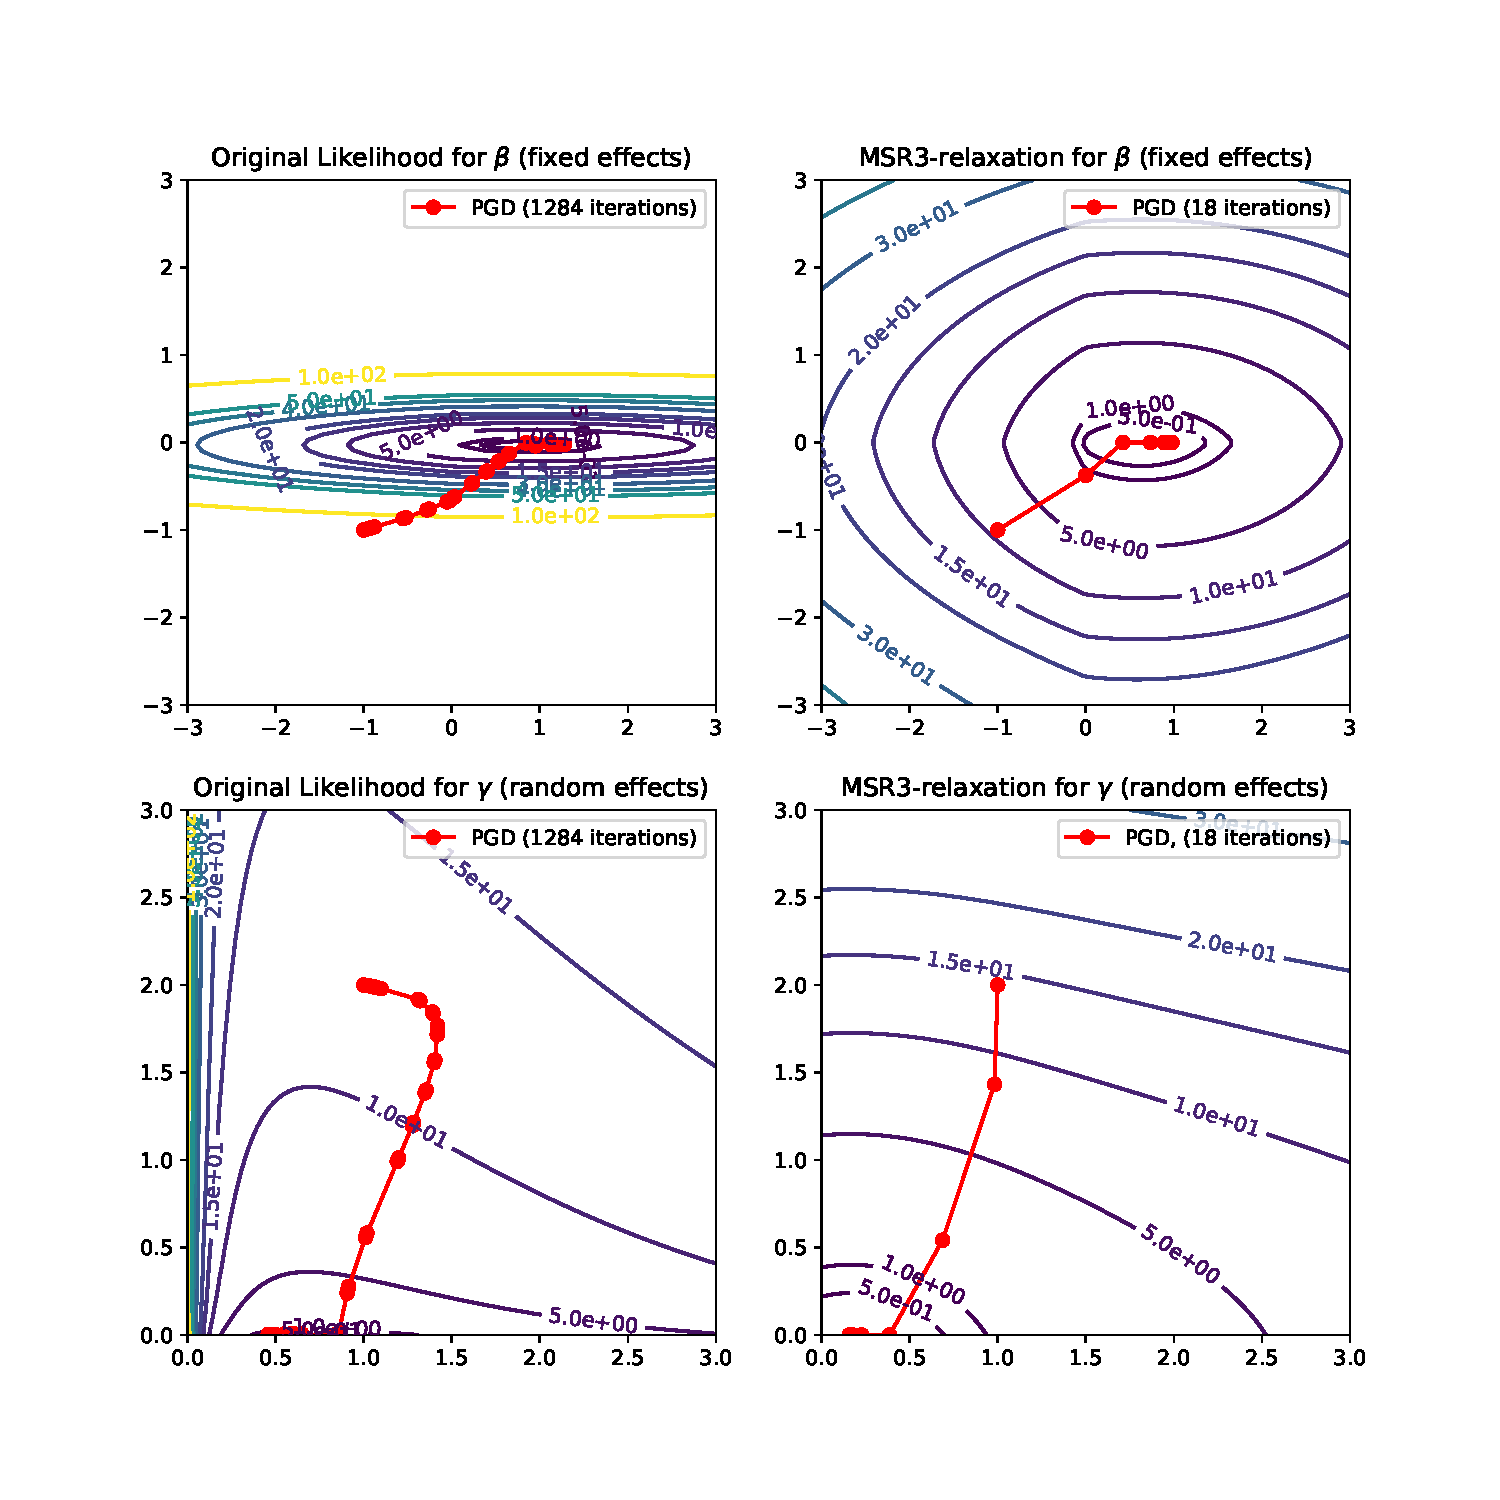
\includegraphics[width=1\textwidth]{Images/intuition_current.pdf}
 %   \caption{Proximal Gradient Descent (PGD) for~\eqref{eq:value_function_optimization} converges far faster than for~\eqref{eq:lme_loss_original_in_x}, because the SR3-value function $u_\eta$ yields more spherical level-sets than original likelihood for both convex components $\beta$ (first row) and non-convex components $\gamma$ (second row). 
    %The effect is particularly strong for $\gamma$-minimizers near the boundary of the constraint region (bottom-left panel).
%    }
 %   \label{fig:geometric_intuition_sr3}
%\end{figure}

\subsection{Variable Selection via MSR3}\label{sec:MSR3}

To develop an approach that is both more efficient and accurate, we extend the SR3 regularization of~\cite{Zheng2019SR3} to LMEs. 
We call the extension MSR3, since we are focusing on mixed effects models. 
Starting with the regularized likelihood~\eqref{eq:lme_loss_original_in_x} we introduce auxiliary parameters designed to discover the fixed and random features: 
\eq{%\label{eq:main opt in x over C}
    \label{eq:lme_loss_sr3}
    \min_{x, w} & \LL(x) + R(w)+ \delta_{\CC}(x) + \kappa_{\eta}(x-w),
%    \\
%    \text{s.t. } & x \in \CC\ .
}
where $\kappa_\eta$ penalizes deviations between $x = (\beta, \gamma)$ and $w = (\hat \beta, \hat \gamma)$, and also guarantees that the objective is convex with respect to the $\gamma$
components of $x$ for sufficiently large $\eta$: \\
\begin{equation}
\label{eq:kappa}
\kappa_\eta (x-w) = \frac{\eta}{2}\|x-w\|^2 = 
%\frac{\eta}{2}\left\| \begin{pmatrix} \beta - \hat \beta \\ \gamma - \hat \gamma\end{pmatrix}\right\|^2
\frac{\eta}{2}\| \beta - \hat \beta \|^2 + 
\frac{\eta}{2}\| \gamma - \hat \gamma\|^2
%\kappa_{\eta} (\beta, \gamma) = \frac{\eta}{2}\|(\beta,\gamma)\|^2 ,
\end{equation}

with $\eta\ge\bar\eta$ where $\bar \eta$ is the weak convexity constant
computed in~\cite[Section 5.1]{Theory1}.
As $\eta \uparrow \infty$, the extended objective~\eqref{eq:lme_loss_sr3} converges in an epigraphical sense to the original objective~\eqref{eq:lme_loss_original_in_x}. 
However, feature selection accuracy does not require this continuation, 
indeed, we show that a fixed 
modest value such as $\eta=1$ can be used~\citep{Zheng2019SR3}.

To understand the algorithm and logic behind the objective~\eqref{eq:lme_loss_sr3}, we define an optimal value function $u_\eta(w)$ and the solution set $S_\eta(w)$:
\eq{
\label{eq:value_function_definition_only_eta}
		u_\eta(w) & = \min_x \ \LL(x) + \delta_{\CC}(x) + \kappa_{\eta}(x-w)\\
		S_\eta(w) & = \argmin_x \LL(x) + \delta_{\CC}(x) + \kappa_{\eta}(x-w).
}
Substituting (\ref{eq:value_function_definition_only_eta}) into (\ref{eq:lme_loss_sr3}) 
%the problem 
transforms (\ref{eq:lme_loss_sr3}) into 
%the problem of optimizing a regularized value function:
\eq{
	\label{eq:value_function_optimization}
	\min_{w} u_\eta(w) + R(w)
}
%Thus at a conceptual level, 
Here we have transformed the original regularized likelihood~\eqref{eq:lme_loss_original_in_x}  %has been transformed 
through relaxation and partial 
minimization to obtain an equivalent problem~\eqref{eq:value_function_optimization} 
for $w$ with the same regularizer. The value function $u_\eta$ encapsulates 
global variational information on the function $\LL(x) + \delta_{\CC}(x)$
relative to $w$.
%Problem~\eqref{eq:value_function_optimization} 
%attempts to find sparse $w$ that are small with respect to $u_\eta$. 

In the case of linear regression, 
the function $u_\eta$ has a closed form solution~\cite{Zheng2019SR3}. However, in both  the linear regression context of~\cite{Zheng2019SR3} 
and in the LME context studied here, we need only compute $S_\eta(w)$ 
in order to optimize~\eqref{eq:value_function_optimization}. 
Indeed, in \cite[Section 5]{Theory1} it is shown that 
there exists a computable $\bar\eta>0$, which we have called the weak convexity constant, such that
$\LL+\delta_\CC+\kappa_\eta(\cdot -w)$ is strongly convex for all 
$\eta>\bar\eta$ regardless of the choice of $w$. This allows us to show
that 
$u_\eta$ is well-defined, 
differentiable, and Lipschitz continuous, with
%and we have a closed form solution for the derivative: 
\begin{equation}\label{eq:grad_value_function_explicit}
\nabla u_\eta(w) = \nabla_w k_\eta(x-w)|_{x = S_\eta(w)}=\eta(w-S_\eta(w)) .  
\end{equation}
%We call $\bar\eta$ the weak convexity constant for 
%$\LL+\delta_\CC+\kappa_\eta(\cdot -w)$.
%where $\nabla_w k_\eta(x-w)$ is computed directly from~\eqref{eq:kappa}. 

Our empirical studies indicate that 
(\ref{eq:value_function_optimization}) has advantages over (\ref{eq:lme_loss_original_in_x})
from an optimization perspective since $u_\eta$ typically has nearly spherical level-sets while keeping the position of minima close to those of $\LL(x)$. This effect is extensively studied and validated for a quadratic loss function in the original work  of \cite{Zheng2019SR3}. 
%we provide empirical evidence that suggests that it also extends to more general non-linear functions, specifically to the marginal likelihood. 
In the center panel of Figure~\ref{fig:summary}, we plot the level-sets of $\LL(x) + \|x\|_1$ (left column) and $u_\eta + \|\cdot\|_1$ (right column) for the same mixed-effect problem. 
%A more symmetrical 
The more spherical geometry of the latter allows the Algorithm \ref{alg:pgd_for_value} 
(described below) to converge in 21 iterations, whereas Algorithm \ref{alg:pgd_for_lme} takes 1284 iterations. The difference is most pronounced when the minimum sits on the boundary of the feasible set, which is always the case for the variable selection problems with sparse support.
%In effect, Algorithm \ref{alg:pgd_for_value} incorporates global variational information 
%about the function $\LL$ while Algorithm \ref{alg:pgd_for_lme}

%The value function $u_\eta(w)$ possesses the following properties: 
%
%\begin{theorem}[Properties of value function optimization]
%\label{thm:properties_of_value_function}
%Let $\eta > 0$, $R(x)$ is level-compact. Then
%\begin{enumerate}
%	\item The solutions for (\ref{eq:value_function_optimization}) always exists when $R(w)$ is level-compact \cite[Theorem 6]{jimtheory}.
%	\item The solution set $S_\eta(w)$ is well-defined, single-valued and continuous \cite[Theorem 9]{jimtheory}
%	\item $u_\eta(w)$ is well-defined and continuous \cite[Theorem 9]{jimtheory}.
%	\item $u_\eta(w)$ is differentiable with $\nabla_w u_\eta(w) = \nabla_w \kappa_{\eta}(\bar{x}-w)$ where $\bar{x} = S_\eta(w)$ \cite[Theorem 11]{jimtheory}
%\end{enumerate}
%\end{theorem}

We apply PGD to optimize the regularized value function $u_\eta$ which yields the iteration 
\eq{
	\label{eq:pgd_for_value_function}
	w^+ = \prox_{\alpha^{-1}R}(w - \alpha\nabla u_\eta(w))
}
The results in \cite{Theory1} show that all components of the iteration~(\ref{eq:pgd_for_value_function}) are well-defined. 
The equivalence of Algorithm \ref{alg:pgd_for_value} and 
\eqref{eq:pgd_for_value_function} is established in the following lemma, 
which extends the relationship studied by~\cite{Zheng2019SR3} to the case of $x = (\beta, \gamma)$. 

%To get a deeper intuition for Algorithm~\ref{alg:pgd_for_value} we make the following remark. 
\begin{lemma}[Equivalence of Algorithms]\label{lem:equivalence}
Algorithm~\ref{alg:pgd_for_value} is equivalent to~\eqref{eq:pgd_for_value_function}. 
\end{lemma}
\begin{proof}
%Specifically, we define $\alpha$ to be block-specific: 
%	\[
%	\alpha = [\underbrace{\eta^{-1}, \dots, \eta^{-1}}_{p}, \underbrace{(\eta + \overline\lambda)^{-1}, \dots (\eta + \overline\lambda)^{-1}}_q]
%	\]
%so that we have
%	\eq{
%		\label{eq:grad_value_function_explicit}
%		\nabla u_\eta(w) = \alpha \odot (\overline{x} - w)|_{\overline{x} = S_\eta(w)}
%	}
%where ``$\odot$'' denotes the Hadamard or element-wise product.  
Substituting~(\ref{eq:grad_value_function_explicit}) into~(\ref{eq:pgd_for_value_function}), 
we see that the iteration~(\ref{eq:pgd_for_value_function}) is equivalent to the alternating minimization scheme outlined in the Algorithm~\ref{alg:pgd_for_value}.
\end{proof}
\begin{algorithm}[H]
\SetAlgoLined
$w = w_0$ \\
 \While{not converged}{
    $x^+ = \arg\min_x \LL(x) + \delta_{\CC}(x) + \kappa_{\eta}(x-w)$ \\
    $w^+ = \prox_{\alpha^{-1} R}(x^+)$
 }
 \caption{\label{alg:pgd_for_value}Proximal Gradient Descent for Value Function}
\end{algorithm}
\smallskip

In \cite[Theorem 6]{Theory1}, it is shown that
for any sequence $\eta_k\uparrow\infty$ the associated optimal solutions $(x^k,w^k)$ 
to (11) satisfy
\(
\mathcal{L}(x^k)+R(w^k)\uparrow 
\inf_{x\in\Rp\times\Rq_+}\mathcal{L}(x)+R(x) \;
\text{with}\; \Vert{x^k-w^k}\Vert\rightarrow 0.
\)
In particular, every cluster point of the sequences $\{x^k\}$ and $\{w^k\}$ are solutions
to \eqref{eq:lme_diagonal_setup}, where such cluster points exist whenever
the function $R$ is coercive, i.e. $\lim_{\norm{x}\uparrow\infty}R(x)=+\infty$.
Just how close $w^k$ is to a solution to \eqref{eq:lme_diagonal_setup} remains
an open question, however, our numerical studies in Section \ref{sec:applications}
show that $\eta$ can be chosen surprisingly small. Indeed, we typically take $\eta=1$.


In the linear regression setting of~\cite{Zheng2019SR3}, 
Algorithm~\ref{alg:pgd_for_value} can be implemented exactly. 
In the nonlinear case, evaluating $x^+$ requires an iterative algorithm. 
For this we use an interior point method which replaces the indicator function
$\delta_\CC$ by a smooth log-barrier term. This allows us to approximate both
$u_\eta$ and its gradient where  
the degree of the approximation is controlled by the convergence 
criteria of the interior point algorithm.  

%The alternating strategy is best suited for the simpler context , where the $x^+$ update has a closed form solution. In the case of~\eqref{eq:lme_loss_sr3}, the regularized loss is convex in $x$ because of the structure of $\kappa_\eta$, but is still nonlinear, and requires an iterative algorithm.  

\paragraph{An Interior Point Method for Approximating $u_\eta$.}

In order to solve for the $x^+$ update in line 2 of Algorithm~\ref{alg:pgd_for_value}, we must optimize a convex loss with linear inequality constraints, that is, 
for a fixed $w = (\hat \beta, \hat \gamma)$, we need to solve 
\begin{equation}
\label{eq:ineqLoss}
\min_{\beta, \gamma} \mathcal{L}(\beta, \gamma) + \kappa_{\eta}(\beta - \hat \beta, \gamma - \hat \gamma) \quad \mbox{s.t.} \quad 0 \leq \gamma. 
\end{equation}
This problem is well suited for an interior point approach~\citep{Kojima1991,Nesterov1994,Wright1997,vanderbei99}. 
%We now describe how to apply IP methods \teal{to solve the inner problem~\eqref{eq:lme_loss_relaxed} with respect to $x = (\beta, \gamma)$, 
%evaluating the value function $u(w)$ in~\eqref{eq:value_function_definition}}. 
%\eqref{eq:lme_loss_original}. 
% when $\LL=\LL_{ML}$. The case where $\LL=\LL_{REML}$ follows a 
% similar pattern.
%To apply IP methods to our problem class, we first 
First, the inequality constraint $0\le\gam$ is relaxed
using the perspective of the negative log, i.e %log-barrier function
$\map{\vphi}{\R^q\times\R}{\R\cup\{\infty\}}$ given by
\[
\vphi(\gam,\mu):=
\begin{cases}
-\mu\sum_{i=1}^q\ln (\gam_i/\mu)&,\ \mu>0,\\
\del_{\R^q_+}(\gam)&,\ \mu=0,\\
+\infty&,\ \mu<0.
\end{cases}
\]
The mapping $\vphi$ is known to be a closed proper convex function and, 
for $\mu>0$, it is
essentially equivalent to the well-known log-barrier function.
%since in this case
%\[
%\phi_\mu(\gam)=q\mu\ln(\mu)-\mu\sum_{i=1}^q\ln (\gam_i).
%\]
For more information on the perspective mapping, its calculus,
and perspective duality, we refer the reader to \cite{ABDFM18,ABF13}.
%\red{Should we mention the perspective of $\psi(\gam)=-\ln (\gam)$, or perhaps the closure of the epi-limit? The connection to the perspective map might be useful since
%we get the joint convexity in $\mu$ and $\gam$.}
We call $\eta$ the coupling parameter and $\mu$ the log-barrier parameter
and write $\phimu(\cdot):=\vphi(\cdot,\mu)$.
%The parameter $0\le\blam$ is fixed and is related to the weak convexity of $\LL$
%discussed in Lemma \ref{lem:LL weak cvx}.
%}
The relaxed problem employs 
auxiliary variables $\tbg$ 
and relaxation parameters $0\le\eta$ and $0\le \mu$
to obtain the problem 
\begin{equation}\label{eq:relax} 
\begin{aligned}%\eq{\label{eq:lme_loss_relaxed}
%\nu_\emu:=	
\min_{\bg, \tbg} & \LL(\beta, \gamma) 
	+\phi_\mu(\gam)+\kappa_\eta(\beta-\tbeta,\gam-\tgam)
%\frac{\eta}{2}\norm{\beta - \tbeta}^2 + \frac{\blam+\eta}{2}\norm{\gamma - \tgamma}^2  
+ R(\tbeta, \tgamma) 
\\
\text{s.t. } & \tgamma \geq 0\ .
\end{aligned}
\end{equation}

We rewrite \eqref{eq:relax} %\eqref{eq:lme_loss_relaxed} 
so as to separate the smooth and nonsmooth components to obtain
\eq{ \label{eq:relax2}
    \min_{\bg, \tbg} & \LL_{\emu}(\bg,\tbg) + R\tbg +\del_{\R^q_+}(\tgam)\ ,
%    \\
%    \text{s.t. } & 0\le\tgam,
}
where 
%$x=(\beta, \gamma)$, 
%$w=(\tbeta, \tgamma)$, $\CC=\R^p\times\R^q_+$, and
%$\LL_\eta$ is defined in \eqref{eq:defn L sub eta}.
\eq{\label{eq:LLlam}
    \LL_{\emu}(\bg, \tbg) := 
    \LL\bg + \phimu(\gam)+\keta(\beta - \tbeta, \gamma - \tgamma).
}
Observe that, for all $\mu,\eta\in\R_+$, $\LL_{\emu},\ \nabla \LL_{\emu}$ and $\nabla^2 \LL_{\emu}$ are continuous
on $(\Rp\times\dom(\phimu))\times(\Rp\times\Rq)$ 
(see Appendix \ref{appendix:derivatives_of_lmm}) 
so that $\LL_{\emu}$ is smooth on its domain.
As in \cite{Zheng2019SR3}, we use the 
decoupling to write \eqref{eq:relax2}
as an iterated optimization problem over the smooth components of the objective.
This yields a representation of the form
\begin{equation}
    \label{eq:relax3}
    \min_{\tbg} \uemu\tbg + R\tbg+\del_{\Rqp}(\tgam),
\end{equation}
where %$w=(\tbeta,\tgam)$ and
\begin{equation}
    \label{eq:value_function_definition}
    \uemu\tbg := \min_{\bg } 
    \LL_{\emu}(\bg, \tbg)\ .
%    \hLL(\bg,\tgam)+ %\del_{\Rqp}(\gam)+
%    \frac{\eta}{2}\norm{\bg-\tbg}^2
    %\LL(x) + \lambda\|x - w\|_2^2 
\end{equation}
This is the formulation of the mixed-effects variable selection problem we study. 
Notice that this value function differs from a simplified 
definition in \eqref{eq:value_function_definition_only_eta}: we replaced 
the linearity constraint with a perspective function and got another parameter $\mu$ due to it. The log-barrier penalty approximates the indicator function to the positive orthant as $\mu$ decreases; indeed, the function $\gamma\mapsto\mu\ln(\gamma)$ epi-converges to the indicator function $\delta_{\mathbb{R}^n_+}(\gamma)$ as $\mu \downarrow 0$ (\cite{rockafellar2009variational}). The penalty (homotopy) parameter $\mu$ is progressively decreased to $0$ as the algorithm proceeds as described below. 
%in the limit minimizing $\mathcal{L}_{\eta,\mu}$ gives the right $x^+$ update in Algorithm~\ref{alg:pgd_for_value}. 
 We refer to \eqref{eq:value_function_definition} when we say ``value function'' from now on.

Our focus is on the optimal value function $\uemu$ which captures global 
variational information about the function $\LL$ over its domain.
In Section~\ref{sec:theory-paper} we show that $\uemu$ has a locally Lipschitz continuous gradient
and that the evaluation of $\uemu$ and $\nabla \uemu$ is accomplished
by optimizing a well conditioned strongly convex function. This
allows us to apply the PGD algorithm to the function $\uemu$ rather than
the function $\LL$. Our numerical studies in Section~\ref{sec:applications} show that the global information 
captured by $\uemu$ significantly improves both the accuracy of the solution
obtained and the overall numerical efficiency of the algorithm. 

%The Lagrangian for~\eqref{eq:log_barrier_relaxation_for_ip} is obtained by dualizing the inequality $\gamma \geq 0$ constraint: 
% Define the objective for \eqref{eq:log_barrier_relaxation_for_ip} by
% \eq{
% 	F_\mu(\beta, \gamma) & = \LL(\beta, \gamma) +  \frac{\lambda_b}{2}\|\beta - \tbeta^{(k)}\|^2_2 + \frac{\lambda_g}{2}\|\gamma - \tgamma^{(k)}\|_2^2 - \mu\sum_{i=1}^{q}\log(\gamma_i) %+ v^T\gamma \\
% }


For $\gamma>0$, the necessary optimality conditions 
for $\mathcal{L}_{\mu,\eta}$ in $\gamma$ give us the relation 
%between dual variables $v$ and the primal variables $\gamma$: 
\eq{
	\nabla_\gamma \mathcal{L}_{\mu,\eta}(\beta,\gamma) = 
	%\begin{bmatrix}
\nabla_\gam \LL(\beta,\gam)+\eta (\gamma - \hat\gamma)
-\mu \Diag{\gam}^{-1}\one
=0,
%		v_1 - \mu/\gamma_1 \\
%		\dots \\
%		v_q - \mu/\gamma_q 
%	\end{bmatrix} = \begin{bmatrix}
%		0 \\
%		\dots \\
%		0 
%	\end{bmatrix} 
%	\implies v_i\gamma_i = \mu \text{ for } i=1,\dots,q.
}
where $\one$ is the vector of all ones of the 
appropriate dimension.
By setting 
\(
v=\nabla_\gam \mathcal{L}_{\mu,\eta}(\beta,\gam)+\eta(\gamma - \hat \gamma),
\) 
we can rewrite this equation as
%This equation can be written in a matrix form as 
\eq{
	\label{eq:complementary_slackness_kkt}
	v\odot\gamma - \mu\one = 0,
}
where $\one$ is the vector of all ones of the appropriate dimension and
``$\odot$'' denotes the Hadamard (or simply element-wise) product.
%Together with the remaining optimality conditions, we obtain a set of nonlinear equations  that form the the KKT system for~\eqref{eq:log_barrier_relaxation_for_ip}:
The complete set of optimality conditions for 
\eqref{eq:value_function_definition} can now be written as
\eq{\label{eq:IP equations}
	G_{\mu,\eta}(v, \beta, \gamma) & 
%	= \begin{bmatrix}
%		\nabla_v F_\mu \\
%		\nabla_\beta F_\mu \\
%		\nabla_\gamma F_\mu 
%	\end{bmatrix} 
:= \begin{bmatrix}
v\odot \gamma - \mu\one \\
\nabla_\beta \LL(\beta, \gamma) + \eta(\beta - \hat \beta) \\
\nabla_\gamma \LL(\beta, \gamma) + \eta(\gamma - \hat \gamma) - v
\end{bmatrix} = 0.
}
We then apply Newton's method to~\eqref{eq:IP equations}, 
that is, in each iteration the search direction $[\Delta v, \Delta \beta, \Delta \gamma]$ solves the linear system
\[
	\nabla G_{\mu,\eta}(v, \beta, \gamma)\begin{bmatrix}
		\Delta v \\
		\Delta \beta \\
		\Delta \gamma
	\end{bmatrix} = -G_{\mu,\eta}(v, \beta, \gamma), \quad
	\nabla G_{\mu, \eta}(v, \beta, \gamma) = \begin{bmatrix}
 		\Diag{\gamma} & 0 & \Diag{v} \\
 		0 & \nabla^2_{\beta\beta}\LL + \eta I & \nabla^2_{\beta\gamma} \LL\\
 		-I & \nabla^2_{\gamma\beta}\LL & \nabla^2_{\gamma\gamma}\LL + (\eta + \overline{\lambda})	 I
 	\end{bmatrix}
\]
and we have used the fact that  $v\odot \gamma=\Diag{v}\gam=\Diag{\gam}v$. 
The exact formulae for the derivatives of $\LL$ are provided in the Appendix~\ref{appendix:derivatives_of_lmm}.

The general structure of the algorithm is as follows.
Given a search direction
$[\Delta v^{(k)}, \Delta \beta^{(k)}, \Delta \gamma^{(k)}]$, 
choose a step of size $\alpha_k>0$
%\eq{
%    \label{eq:ip_step}
%	v^{(k+1)} & = v^{(k)} + \alpha_k \Delta v \\
%	\gamma^{(k+1)} & = \gamma^{(k)} + \alpha_k \Delta\gamma \\
%	\beta^{(k+1)} & = \beta^{(k)} + \alpha_k \Delta \beta
%}
%with $\alpha_k$ 
so that the update
\[
\begin{pmatrix}
v^{(k+1)}& \beta^{(k+1)}& \gamma^{(k+1)}
\end{pmatrix}
=
\begin{pmatrix}
v^{(k)}& \beta^{(k)} &\gamma^{(k)}
\end{pmatrix}
+\alf_k
\begin{pmatrix}
\Delta v^{(k)} & \Delta\beta^{(k)}& \Delta\gamma^{(k)}
\end{pmatrix}
\]
satisfies the conditions
% chosen to satisfy positivity and sufficient descent conditions:
\[
\begin{aligned}
	\text{\textit{Positivity:}} \qquad & \gamma^{(k+1)} > 0,\ v^{(k+1)} > 0 \\
	\text{\textit{Sufficient Descent:}}\qquad & \| G_\emu(v^{(k+1)}, \beta^{(k+1)}, \gamma^{(k+1)})\| \leq 0.99\|G_\emu(v^{(k)}, \beta^{(k)}, \gamma^{(k)})\|,
\end{aligned}
\]
where the parameter $0.99$ is used to bias toward the acceptance of a full Newton step.
At each iteration the relaxation parameter $\mu$ is updated by the formula 
\( %\eq{
%    \label{eq:ip_mu_update}
    \mu^{(k+1)} = {v^{(k)}}^T\gamma^{(k)}/q,
\) %}
where ${v^{(k)}}^T\gamma^{(k)}$ is the duality gap at
iteration $k$. The algorithm terminates when the criteria 
\[
\begin{aligned}
\|G_{\mu,\eta}(v^{(k+1)}, \beta^{(k+1)}, \gamma^{(k+1)})\| &\leq \text{\texttt{tol}}\\
\mu &\leq  \text{\texttt{tol}} 
\end{aligned}
\]
are both satisfied, so the interior point problem is nearly stationary, and closely approximates the original problem~\eqref{eq:ineqLoss}.
MSR3 is summarized in Algorithm~\ref{alg:MSR3}, which approximates Algorithm~\ref{alg:pgd_for_value} as the tolerance goes to $0$. 
In the numerical experiments, we use $\text{\texttt{tol}} = 10^{-5}$, and accuracy does not change as the tolerance parameter decreases.  

\begin{algorithm}[H]
\SetAlgoLined
$w = w_0$ \\
 \While{not converged}{
    $x^+ \; \mbox{satisfies }\;  \|G_{\mu,\eta}(v^+, x^+)\| \leq \text{\texttt{tol}}, \; \mu \leq \text{\texttt{tol}} $\\
    $w^+ = \prox_{\alpha^{-1} R}(x^+)$
 }
 \caption{\label{alg:MSR3} MSR3}
\end{algorithm}



\paragraph{Positive Approximation of the Hessian}
For many datasets the weak convexity constant $\overline \eta$ can be extremely large 
and difficult to compute. However, if $ \eta$ is too small 
$\nabla^2_{\gamma\gamma}\LL_{\mu,\eta}(\beta, \gamma)$ is 
negative-(semi)definite. Negative definite Hessians can hamper the convergence of 
second-order methods (e.g., see \cite{nocedal2006numerical}). 
Therefore, one must take care in selecting $\eta$. For this, we recall from
\cite[Lemma 3]{Theory1} that
\[
\nabla^2\LL{(\beta,\gam)}=\sum_{i=1}^m
S_i^T\begin{bmatrix}X_i^T\\ -Z_i^T\end{bmatrix}
\Omega_i(\gam)^{-1}
\begin{bmatrix}X_i& -Z_i\end{bmatrix}S_i
-\begin{bmatrix}
0&0\\ 0& \half(Z_i^T\Omega_i(\gam)^{-1}Z_i)^{\circ2}
\end{bmatrix}.
\]
This implies that negative eigenvalues for the Hessian must arise from the
Hessian with respect to $\gamma$,
$\nabla^2_{\gamma\gamma}\LL(\beta, \gamma)$, and more specifically, the
term $(Z_i^T\Omega_i(\gam)^{-1}Z_i)^{\circ2}$. 
A positive semidefinite approximation to the Hessian is obtained by simply dropping this term. 


\subsection{Relaxation and Efficient Algorithms: MSR3 and MSR3-Fast }
\label{sec:synthetic}

While algorithm~\eqref{alg:pgd_for_value} is modular, it requires solving a nonlinear optimization problem in $x = (\beta, \gamma)$ for each single update
of $w = (\hat \beta, \hat \gamma)$. To make the implementation as efficient as possible, we designed a more balanced updating scheme, that 
alternates Newton iterations as described in the interior point algorithm with $w$ updates. We update $w$ whenever we are sufficiently close 
to the `central path' in the interior point method, a condition that can be checked rigorously using optimality conditions. 
This scheme is detailed in Algorithm~\ref{alg:pgd_for_value_function_fast}.

In designing Algorithm~\ref{alg:pgd_for_value_function_fast}, we chose a particular central path parameter, $\tau = 0.5$ in line 8, 
that controls how far the interior point method needs to proceed before we take a proximal gradient step. We explored the effect of this parameter
on performance and timing in Section~\ref{ch:msr3_sensitivity_analysis} and found that it did not have any effect on either for values between $0.1$ and $0.9$. MSR3-fast 
was competitive with respect to time compared to PGD and PGD with line search (also as reported in Chapter~\ref{ch:msr3_sensitivity_analysis}) for problems up to 1000 features. 

\begin{algorithm}[!ht]
\SetAlgoLined
$\texttt{progress}\leftarrow \textbf{True}$; \quad \texttt{iter = 0}; \\
$\beta^+, \tbeta^+\leftarrow\beta_0$; 
\quad $\gamma^+, \tgamma^+\leftarrow\gamma_0$;  
\quad $v^+ \leftarrow 1 \in \R^q$; 
\quad  $\mu \leftarrow \frac{{v^+}^T\gamma^+}{10 q}$\\
 \While{\texttt{iter} $<$ \texttt{max\_iter}  \ and \ $\|G_\emu(\beta^+, \gamma^+, v^+)\|$ $>$ \texttt{tol}   \ and  \ \texttt{progress} \\}{
    $\beta \leftarrow \beta^+$; \quad $\gamma \leftarrow \gamma^+$; \quad $\tbeta \leftarrow \tbeta^+$; \quad $\tgamma \leftarrow \tgamma^+$ \\
%    $A \leftarrow \nabla G_\emu((\beta, \gamma, v), (\tbeta, \tgamma))$\\
  %  $b \leftarrow G_\emu((\beta, \gamma, v), (\tbeta, \tgamma))$\\
    $[dv, d\beta, d\gamma] \leftarrow  \nabla G_\emu((\beta, \gamma, v), (\tbeta, \tgamma))^{-1}  G_\emu((\beta, \gamma, v), (\tbeta, \tgamma))$ \tcp*[f]{Newton Iteration}\\ 
    $\alpha \leftarrow 0.99\times\min\left(1, -\frac{\gamma_i}{d\gamma_i}, \forall i :\ d\gamma_i < 0\right)$\\
    $\beta^+ \leftarrow \beta + \alpha d\beta$; \quad $\gamma^+ = \gamma + \alpha d\gamma$; \quad  $v^+ \leftarrow v + \alpha dv$\\
    \If{$\|\gamma^+\odot v^+ - q^{-1}{\gamma^+}^Tv^+ \mathbf{1}\| > 0.5q^{-1}{v^+}^T\gamma^+$}{
  %  	\tcp*[h]{Not in the neighborhood of the central path yet}\\
    	continue \tcp*[f]{Keep doing Newton iterations}\\
    }
    \Else{ 
        $\tbeta^+ = \prox_{\alpha R}(\beta^+)$;
        \    $\tgamma^+ = \prox_{\alpha R + \delta_{\R_+}}(\gamma^+)$; 
        \    $\mu = \frac{1}{10}\frac{{v^+}^T\gamma^+}{q}$ \tcp*[f]{Near central path} 
    }
%	\tcp*[h]{Keep iterating until convergence} \\
    \texttt{progress} = ($\|\beta^+ - \beta\| \geq \text{tol}$ or $\|\gamma^+ - \gamma\|  \geq \text{tol}$ or $\|\tbeta^+ - \tbeta\| \geq \text{tol}$ or $\|\tgamma^+ - \tgamma\| \geq \text{tol}$)\\
    \texttt{iter += 1}
 }
 \Return{$\tbeta^+$, $\tgamma^+$}
 \caption{\label{alg:pgd_for_value_function_fast}MSR3-fast (Optimized Proximal Gradient Descent for the Value function)}
\end{algorithm}


\section{Verifications}
\label{sec:applications}

\subsection{MSR3 for Covariate Selection}
\label{ch:sr3_l1}

\begin{table}
\centering
\begin{tabular}{lllll}
\toprule
     & Model &    PGD &    MSR3 & MSR3-fast \\
Regularizer & Metric &        &        &       \\
\midrule
L0 & Accuracy &   0.89 &   \textbf{0.92} &  \textbf{0.92} \\
     & Time &  41.68 &  88.54 &  \textbf{0.13} \\
L1 & Accuracy &   0.73 &   \textbf{0.88} &  \textbf{0.88} \\
     & Time &  38.39 &   9.13 &  \textbf{0.13} \\
ALASSO & Accuracy &   0.88 &   \textbf{0.92} &  0.91 \\
     & Time &  34.55 &  65.19 &  \textbf{0.12} \\
SCAD & Accuracy &   0.71 &   \textbf{0.93} &  0.92 \\
     & Time &  77.62 &  84.67 &  \textbf{0.17} \\
\bottomrule
\end{tabular}

\caption{\label{table:comparison_of_algorithms} Comparison of performance of algorithms measured as accuracy of selecting the correct covariates and run-time. The L0 strategy stands out 
over other standard regularizers. MSR3 improves performance significantly for all regularizers, while MSR3-fast improves convergence speed while preserving the 
accuracy of MSR3.  
More detailed results are in the Table \ref{table:detailed_comparison_of_algorithms} of Appendix \ref{appendix:detailed_comparison}.}
\end{table}

\begin{figure}
    \centering
	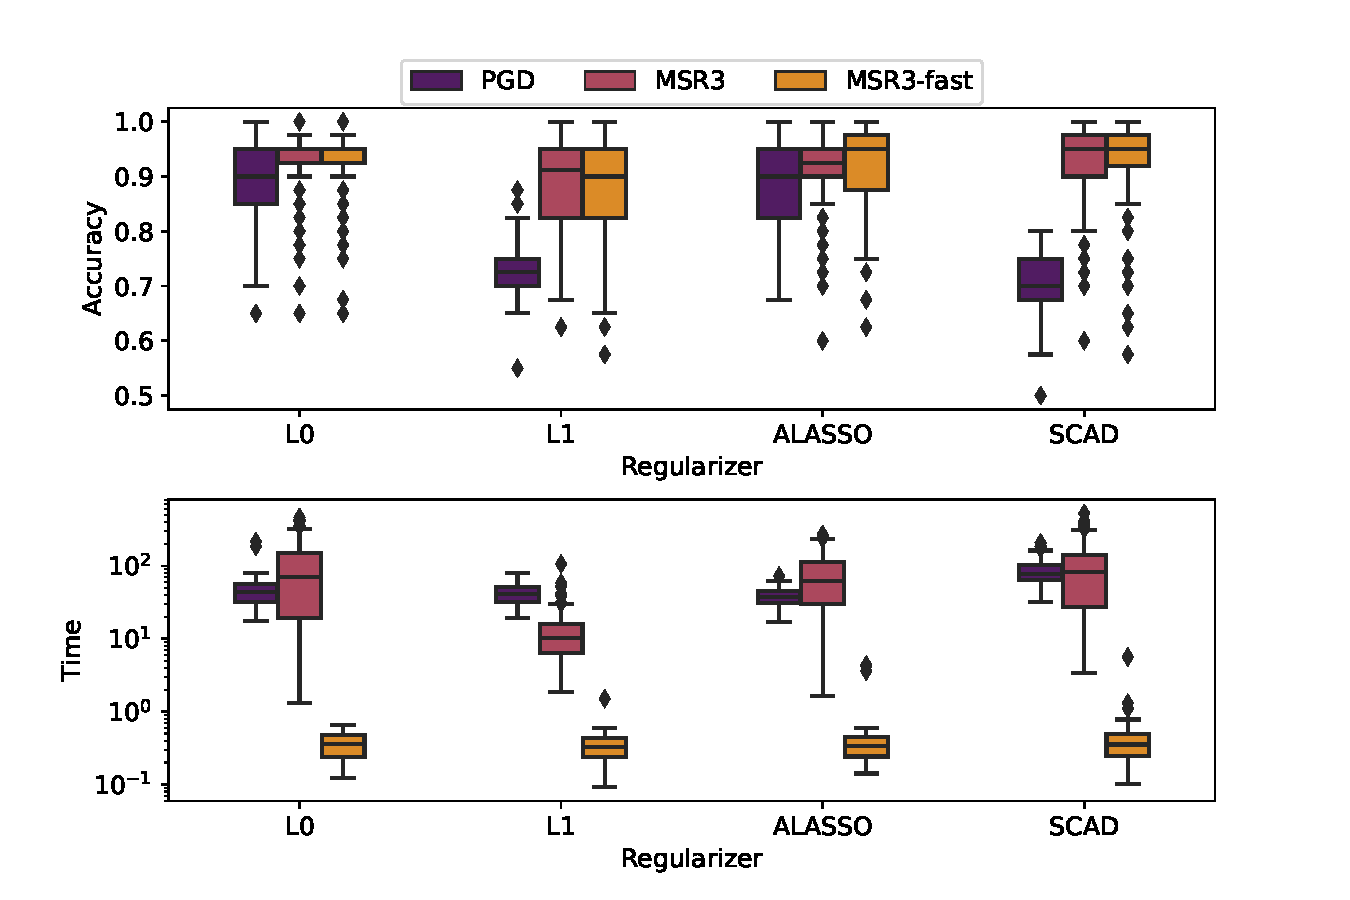
\includegraphics[width=0.8\textwidth]{figures/benchmark}
	\caption{\label{fig:box_with_whiskers_for_synthetic_data}	Feature selection accuracy and execution time in seconds for PGD 
	(Algorithm \ref{alg:pgd_for_lme}), 
	MSR3 (Algorithm \ref{alg:pgd_for_value}), and MSR3-fast
	(Algorithm \ref{alg:pgd_for_value_function_fast}) with various regularizers. 
	MSR3-Fast has the same accuracy as 
	MSR3 and significantly decreases computation time.}
\end{figure}

In this section we compare
%compare the numerical performance 
the feature selection accuracy and the numerical efficiency of Algorithms 
\ref{alg:pgd_for_lme} and 
\ref{alg:pgd_for_value_function_fast} when using the 
LASSO, A-LASSO, SCAD, and L0 sparsity regularizers.
We begin by describing how the data is generated for our numerical simulations 
followed by a description of how the  
regularization parameter $\lambda$ and the coupling parameter $\eta$  were chosen.
Our experiments on real data are presented in Section \ref{sec:real}.

%show the performance of the `regularization-agnostic' feature selection method, and also show that MSR3 improves performance across different regularization strategies. Specifically, we compare the feature selection accuracy and numerical efficiency of Algorithms  \ref{alg:pgd_for_lme} and 
%\ref{alg:pgd_for_value_function_fast} 
%with LASSO, A-LASSO, CAD, SCAD, and L0. 

%\paragraph{LASSO path} The LASSO path is a set of solutions $x$ parametrized by $\lambda$, where $\lambda$ is sweeping over its range from $\lambda = 0$ to $\lambda \to \infty$, until no parameters are included in the model. It's known that a classic LASSO tends to include false positives early along the path (\cite{Su2017}).


\paragraph{Experimental Setup.} The number of fixed effects $p$ and random effects $q$ are set at $20$ with $\beta = \gamma = [\frac{1}{2}, \frac{2}{2}, \frac{3}{2}, \dots, \frac{10}{2}, 0, 0, 0, \dots, 0]$, i.e. the first 10 covariates are increasingly important and the last 10 covariates are not. The data is generated as 
\[
\begin{aligned}
y_i &= X_i\beta + Z_iu_i + \varepsilon_i, \quad  \varepsilon_i \sim \NN(0, 0.3^2 I) \\
X_i &\sim \NN(0, I)^p, \quad Z_i = X_i \\ 
u_i& \sim \NN(0, \Diag{\gamma}),\\ 
\end{aligned}
\]
with 9 groups of sizes $[10, 15, 4, 8, 3, 5, 18, 9, 6]$. 
The data generation is repeated 100 times in order to estimate
the uncertainty bounds. The smallest non-zero components in the generated signals are just above the level of observation noise. 
%\red{We need to say something about "the smallest non-zero components are such that they are just above the noise from observation error"}

\begin{figure}
\center
		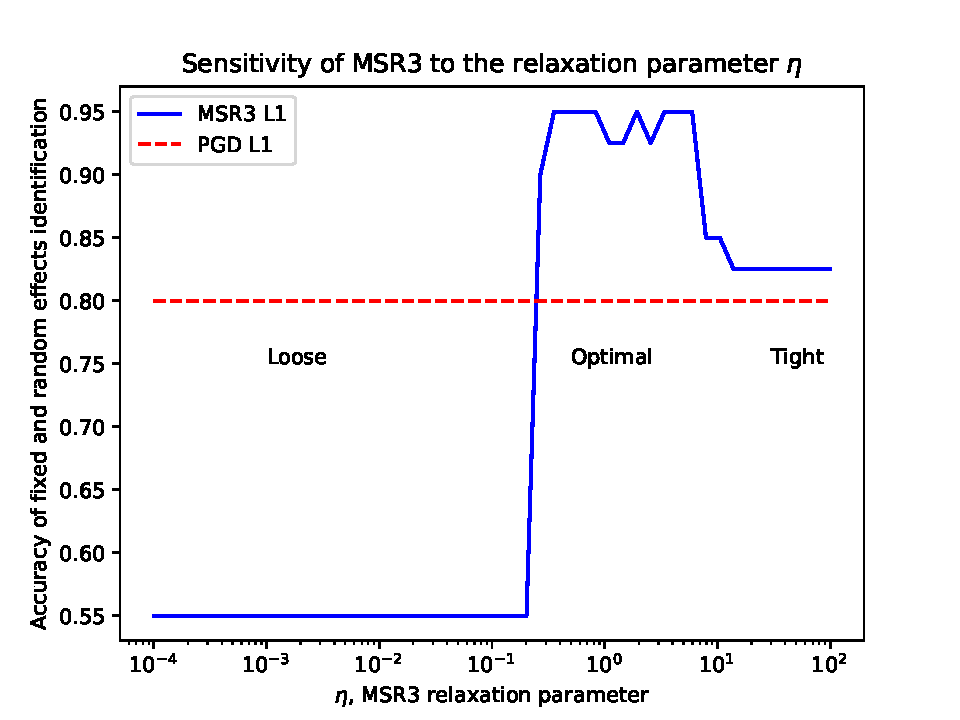
\includegraphics[width=9.5cm]{figures/eta_L1.pdf}
		\caption{Dependence of model performance on the relaxation $\eta$ for a sample problem.}\label{fig:eta}
\end{figure}
	

	
\paragraph{Parameter Selection.} The regularization parameter $\lambda$ 
multiplying $R$ and the 
coupling parameter $\eta$ restricting the difference between 
$(\beta,\gamma)$ and $(\tbeta,\tgam)$ are chosen to maximize a classic 
BIC criterion from \cite{Jones2011}. 
We set a log-uniform grid of 20 candidate values for the parameter $\eta \in [10^{-3}, 10^2]$. For each value of $\eta$,
the BIC is optimized using a golden search in $\lambda \in [0, 10^5]$. The final values of $\eta$ and $\lambda$ are  chosen
to maximize the BIC criterion.
	
	Figure \ref{fig:eta} shows the dependence of accuracy on the values of $\eta$ for the first data set generated in our test set. There are three distinct regions, corresponding to loose, moderate, and tight levels of coupling. When $\eta$ is small the coupling term does not have sufficient strength and the training does not progress far from the initial point (a fully dense vector \textbf{1} in this case). When the coupling is tight, the level-sets and minimizers are closer to those of the the original problem. For the values in between, the coupling significantly improves the model's accuracy. 
These results are consistent with experiments in the sparse linear regression setting~\cite{Zheng2019SR3}. 

\paragraph{Results.}
The experimental results are presented in the Table \ref{table:comparison_of_algorithms} and Figure~\ref{fig:box_with_whiskers_for_synthetic_data}. MSR3 improves the selection accuracy of most regularization techniques 
described in Table \ref{table:proxes}, showing a near-perfect performance, while converging two orders of magnitude faster in wall-clock time. 

\paragraph{Comparison to \texttt{glmmLasso} and \texttt{lmmLasso}.}
We used \cite[Table 3]{Buscemi2019Survey} as a reference 
for feature selection libraries. Of the 17 entries mentioned, the four libraries that successfully ran on our synthetic data described above were  packages \texttt{glmmLasso}\footnote{\href{https://rdrr.io/cran/glmmLasso/man/glmmLasso.html}{https://rdrr.io/cran/glmmLasso/man/glmmLasso.html}} (\cite{groll2014variable}), \texttt{lmmLasso}\footnote{\href{https://rdrr.io/cran/lmmlasso/}{https://rdrr.io/cran/lmmlasso/}}(\cite{schelldorfer2011estimation}), \texttt{fence}\footnote{\href{https://rdrr.io/cran/fence/}{https://rdrr.io/cran/fence/}} (\cite{jiang2008fence}) and \texttt{PCO} (\cite{lin2013pco}) libraries. \texttt{fence} caused a memory overflow on the experimental system during the performance evaluation on the datasets described above. We could not evaluate {\texttt{PCO} because
it did not support  datasets where the total number of random effects $mq$ exceeded the total number of observations $n$. We compare performance of MSR3 
(available through the open source \texttt{pysr3} library) 
to the performance of the \texttt{R} packages \texttt{glmmLasso}\footnote{\href{https://rdrr.io/cran/glmmLasso/man/glmmLasso.html}{https://rdrr.io/cran/glmmLasso/man/glmmLasso.html}} (\cite{groll2014variable}) and \texttt{lmmLasso}\footnote{\href{https://rdrr.io/cran/lmmlasso/}{https://rdrr.io/cran/lmmlasso/}} (\cite{schelldorfer2011estimation}) which are the functionally closest libraries available
} online. As of this writing, \texttt{glmmlasso} does not allow the user to specify $\Gamma$ as a diagonal matrix.  Since the diagonal specification simplifies the problem, this puts \texttt{glmmlasso} package at a disadvantage in our numerical comparison. We evaluate all algorithms' performance on the same set of problems as described above. We tuned the hyperparameters of \texttt{glmmLasso} and \texttt{lmmLasso} by minimizing the BIC scores provided by the libraries over $\lambda \in [0, 10^5]$. The results are presented in Table \ref{table:glmmlasso}. Overall, MSR3 executes, on average, 5 times faster in wall-clock time than \texttt{glmmLasso} and 60 times faster than \texttt{lmmLasso} and shows much higher accuracy in selecting correct fixed and random effects simultaneously. 
{The accuracy of \texttt{glmmLasso} is lower relative to the other libraries' scores likely due to its BIC selection criterion choosing dense models.} The package \texttt{lmmLasso} supports the diagonal specification of $\Gamma$, thus allowing a direct comparison with the scores from \texttt{pysr3}.  \texttt{lmmLasso} yields a competitive accuracy of selecting random effects but \texttt{lmmLasso} provides dense solutions for fixed effects $\beta$ for chosen values of $\lambda$. 

\begin{table}[h]
\centering
\resizebox{\columnwidth}{!}{\begin{tabular}{lrrrr}
\toprule
Algorithm & Units (perc. / 100 runs) &         MSR3-Fast ($\ell_1$)&         glmmLasso &            lmmLasso \\
\midrule
Accuracy &\% (5\%-95\%)    &        {\bf 88 (72-98)} &        48 (42-55) &          66 (55-73) \\
FE Accuracy &\% (5\%-95\%) &      {\bf 86 (64-100)} &        52 (40-66) &          47 (45-55) \\
RE Accuracy &\% (5\%-95\%) &       {\bf 91 (74-100)} &        45 (45-45) &         84 (55-100) \\
F1          &\% (5\%-95\%)&        {\bf 89 (73-97)} &        63 (60-66) &           65 (0-77) \\
FE F1       &\% (5\%-95\%)&       {\bf 88 (69-100)} &        64 (57-70) &           57 (0-64) \\
RE F1       &\% (5\%-95\%)&       {\bf 90 (73-100)} &        62 (62-62) &          78 (0-100) \\
Time        &sec. (5\%-95\%)&  {\bf 0.19 (0.14-0.24)} &  1.37 (0.78-1.89) &  11.51 (5.35-23.66) \\
Iterations  & num. (5\%-95\%)&        {\bf 34 (28-45)} &        50 (33-77) &             - \\
\bottomrule
\end{tabular}
}
\caption{\label{table:glmmlasso} Comparison of performance of MSR3-Fast for $\ell_1$ regularizer vs \texttt{glmmLasso}. MSR3-Fast executes 5 times faster in wall time and has higher accuracy of selecting correct covariates. 
%Importantly, the accuracy of \texttt{glmmLasso} is likely skewed downwards due to BIC selection criterion choosing dense ultimate models and due to the missing option to constrain the matrix $\Gamma$ to be diagonal. \texttt{lmmLasso} supports the diagonal specification of $\Gamma$ which translates into a competitive quality of selecting random effects. However, while finding sparse fixed effects, \texttt{lmmLasso} provides dense solutions for fixed effects $\beta$.
}
\end{table}

\subsection{Scalability and Sensitivity Analysis}
\label{ch:msr3_sensitivity_analysis}
\subsubsection{Scalability}
We tested the scalability of the new approach (MSR3-fast) compared to proximal gradient descent and proximal gradient descent with line search. To do this, chose an initially small problem and we scaled the number of features in the data from 100 to 1000, while scaling the number of observations proportionally, and tested the time to completion 
of these three methods, averaged over 100 replicates. Namely, each problem had 8 groups of $10A$ observations each, $\beta$ and $\gamma$ had $20A$ features equally split between 0 and 1. To get the problems of different sizes we assigned $A$ to be 1, 2, 5, 10, 20, 50, and 100, and for each choice of A we generated 100 random problems. Since MSR3-fast has a relaxation parameter $\eta$, we evaluated MSR3-fast across different $\eta$ values to also test the effect of $\eta$ on timing. For each experiment, we also computed 
the accuracy of the feature selection, to make sure that there was no degradation in performance. The results are presented in Tables~\ref{table:scalability_time} and~\ref{table:scalability_accuracy}.  
In terms of timing, we indeed see a superlinear increase in computational complexity with respect to the number of features. Nonetheless, MSR3-fast is competitive with the alternatives across the experiments, and the results are far more accurate. 
Larger problems could likely significantly benefit from iterated solvers within the interior point framework. 

\begin{table}[ht]
	\centering
    \resizebox{\columnwidth}{!}{\begin{tabular}{l||lllllll|l|l}
\toprule
Algorithm & \multicolumn{7}{l}{MSR3-Fast} &       PGD & PGD-LineSearch \\
$\eta$ &     0.01  &    0.05  &    0.10  &    0.50  &    1.00  &     5.00  &     10.00 &    &         \\
\hline \hline 
\# Features &           &          &          &          &          &           &           &           &                \\
100                &     0m 7s &    0m 7s &    0m 7s &    0m 6s &    0m 7s &     0m 8s &    0m 10s &    2m 44s &         4m 44s \\
200                &    0m 36s &   0m 39s &   0m 36s &   0m 39s &   0m 39s &    0m 49s &     1m 8s &    7m 43s &        11m 28s \\
400                &     5m 2s &   4m 51s &   4m 34s &   4m 26s &   5m 16s &    7m 33s &   10m 38s &   47m 46s &        12m 36s \\
1000               &   59m 10s &  57m 12s &  60m 30s &  69m 57s &  68m 55s &  111m 31s &  139m 47s &  469m 16s &         55m 8s \\
\bottomrule
\end{tabular}
}
    \caption{Execution time for feature selection problems of varying sizes. Each cell shows total time, including grid-search with respect to the sparsity parameter $\lambda$. Each cell shows averaged value over 100 randomly-generated problems.}
    \label{table:scalability_time}

\end{table}

\begin{table}[ht]
	\centering
    %\resizebox{\columnwidth}{!}{}
    \begin{tabular}{l||rrrrrrr|r|r}
\toprule
Algorithm & \multicolumn{7}{l}{MSR3-Fast} &   PGD & PGD-LineSearch \\
$\eta$ &     0.01  & 0.05  & 0.10  & 0.50  & 1.00  & 5.00  & 10.00 &   &           \\
\hline \hline
\# Features &           &       &       &       &       &       &       &       &                \\

100                &      0.94 &  0.94 &  0.95 &  0.94 &  0.91 &  0.86 &  0.84 &  0.77 &           0.77 \\
200                &      0.99 &  0.99 &  0.99 &  0.98 &  0.98 &  0.97 &  0.95 &  0.78 &           0.82 \\
400                &      0.99 &  0.99 &  0.99 &  0.99 &  0.99 &  1.00 &  1.00 &  0.80 &           0.84 \\
1000               &      0.99 &  0.98 &  0.98 &  0.98 &  0.98 &  1.00 &  1.00 &  0.83 &           0.87 \\
\bottomrule
\end{tabular}

    \caption{Accuracy of feature selection problems of varying sizes. Each cell shows averaged value over 100 randomly-generated problems.}
    \label{table:scalability_accuracy}
\end{table}


\subsubsection{Closeness to the Central Path for IP}
The $\tau$ parameter of MSR3-fast controls how close the interior point method gets to the central path before taking a prox-gradient step. This is a heuristic parameter in the algorithm, and to understand its impact we tested 
the sensitivity of the execution time and accuracy for a problem with 200 features for four selections of relaxation parameter $\eta$. The problems were identical to those from the second row of Table~\ref{table:scalability_time}. The results are reported in Tables~\ref{table:central_path_time} and~\ref{table:central_path_accuracy}. 
Neither time nor accuracy were affected by $\tau$ across the levels of $\eta$. 

\begin{table}[ht]
	\centering
    \begin{tabular}{l||llll}
\toprule
Algorithm & \multicolumn{4}{l}{MSR3-Fast} \\
$\eta$ &     0.01  &   0.10  &   1.00  &   10.00 \\
\hline \hline
$\tau$ &           &         &         &         \\
0.1 &    0m 41s &  0m 40s &  0m 41s &  1m 12s \\
0.3 &    0m 35s &  0m 36s &  0m 38s &   1m 1s \\
0.5 &    0m 34s &  0m 35s &  0m 36s &  0m 57s \\
0.7 &    0m 33s &  0m 33s &  0m 35s &  0m 59s \\
0.9 &    0m 33s &  0m 33s &  0m 35s &  0m 52s \\
\bottomrule
\end{tabular}

    \caption{Execution time of MSR3-fast for different values of $\tau$ - a parameter that controls how close the IP needs to be to the central path before doing a projection step. Each cell shows total time, including grid-search with respect to the sparsity parameter $\lambda$. Each cell shows averaged value over 100 randomly-generated problems.}
    \label{table:central_path_time}
\end{table}

\begin{table}[ht]
	\centering
    %\resizebox{\columnwidth}{!}{}
    \begin{tabular}{l||rrrr}
\toprule
Algorithm & \multicolumn{4}{l}{MSR3-Fast} \\
$\eta$ &     0.01  & 0.10  & 1.00  & 10.00 \\
\hline \hline
$\tau$ &           &       &       &       \\
0.1 &      0.99 &  0.99 &  0.99 &  0.95 \\
0.3 &      0.99 &  0.99 &  0.98 &  0.95 \\
0.5 &      0.99 &  0.99 &  0.98 &  0.95 \\
0.7 &      0.99 &  0.99 &  0.98 &  0.95 \\
0.9 &      0.99 &  0.99 &  0.98 &  0.95 \\
\bottomrule
\end{tabular}

    \caption{Accuracy of MSR3-fast for different values of $\tau$ - a parameter that controls how close the IP needs to be to the central path before doing a projection step. Each cell shows averaged value over 100 randomly-generated problems.}
    \label{table:central_path_accuracy}
\end{table}




\subsection{Application to Real Data: Anxiety and Depression as a Result of Bullying Victimization}
\label{sec:real}

\begin{figure}
    \centering
	\caption{\label{fig:bullying_data_random_feature_selection}Validation of Random Feature Selection for Bullying Data from GBD 2020. 
	Left panel shows coefficient paths across numbers of nonzero covariates allowed in the model using the $\ell_0$ regularizer. 
	Right panel evaluates each choice against expert knowledge. 
	The algorithm picks seven historically significant covariates and two historically insignificant, for the model selected using the BIC criteria. 
	See the Appendix \ref{appendix:bullying_covariates} for covariates description and assessment of significance.}
	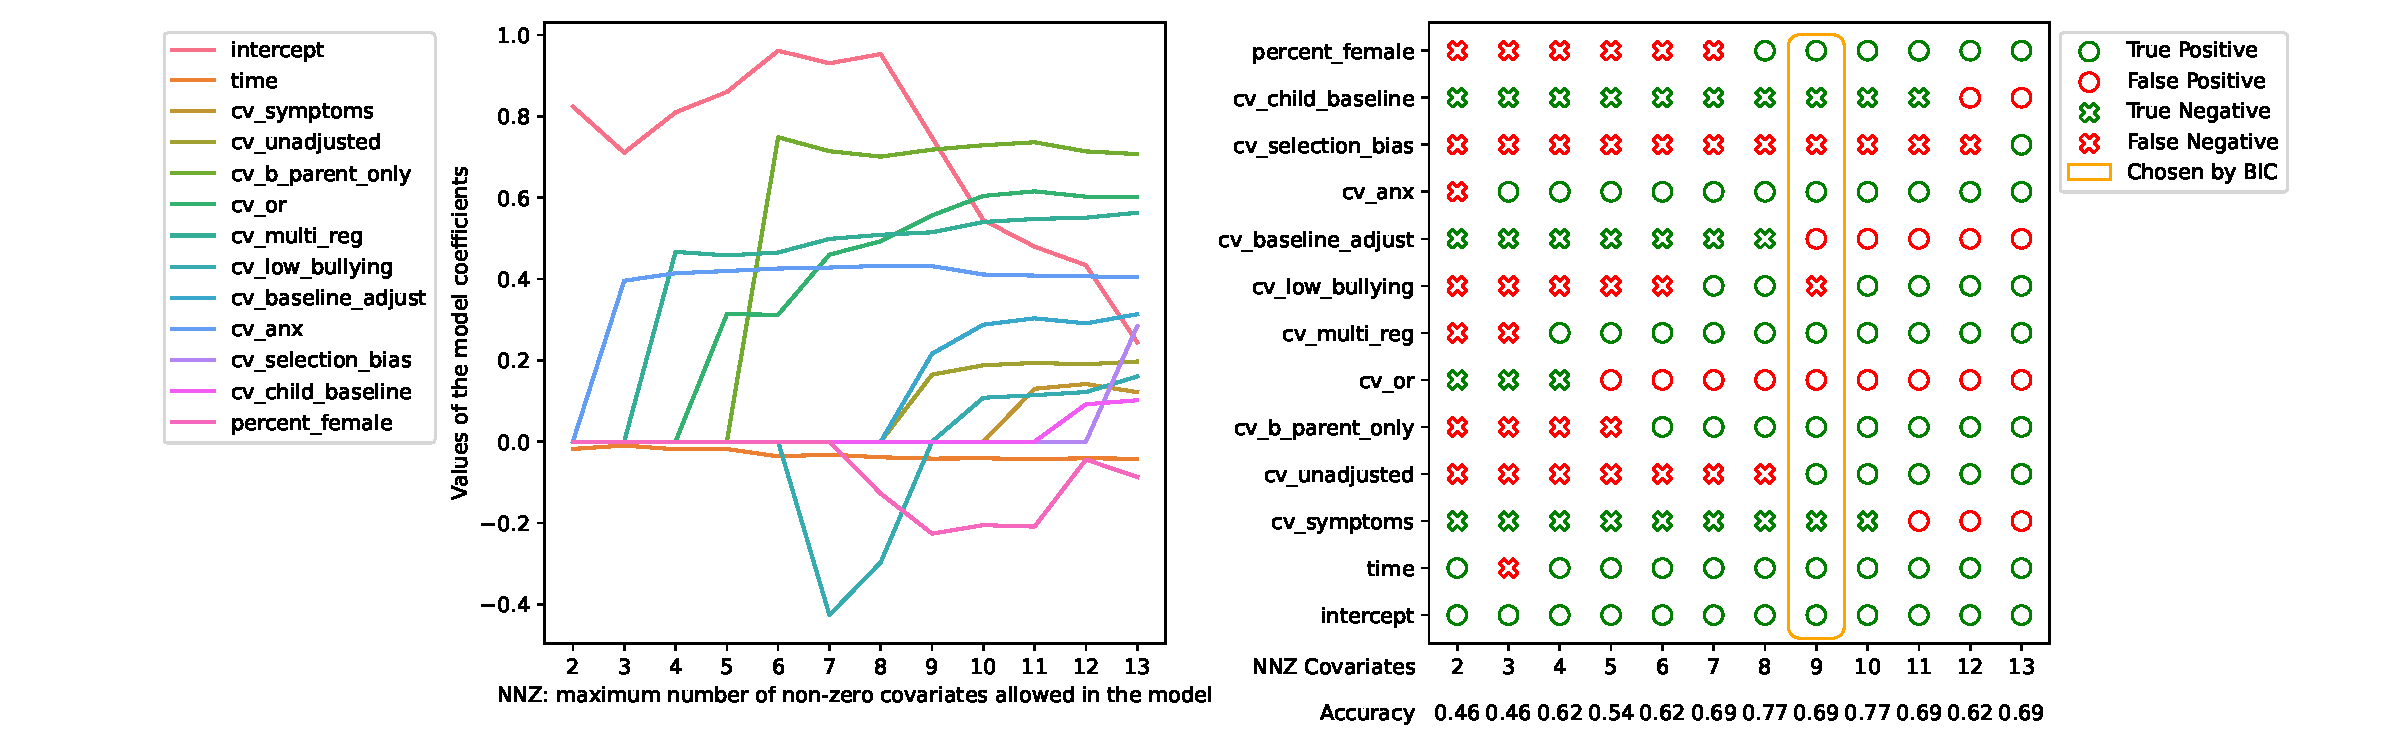
\includegraphics[width=1\textwidth]{figures/bullying_data_assessment_selection}
\end{figure}

In this section we validate the MSR3-empowered $\ell_0$-regularized mixed-effect model ($R(x) = \delta_{\|x\|_0 \leq k}$ from Table \ref{table:proxes}) by using it to identify the most important covariates in real data on relative risk of anxiety and depressive disorders depending on the exposure to bullying in young age\footnote{Institute for Health Metrics and Evaluation (IHME). Bullying Victimization Relative Risk Bundle GBD 2020. Seattle, United States of America (USA), 2021.}. This research has been a part of Global Burden of Diseases study for the last several years. The end goal  is to estimate the burden 
{through disability adjusted life years} (DALYs)~\citep{murray1997understanding}
of major depressive disorder (MDD) and anxiety disorders that are caused by bullying. For this risk factor, the exposure is primarily concentrated in childhood and adolescents, but the risk for MDD and anxiety disorders is anticipated to continue well into adulthood. This elevated risk is, however, expected to decrease with time as other risk factors come into play in adulthood (unemployment, relationship issues, etc.). To accommodate this, the research team uses the models which estimate the relative risk (RR) of MDD and anxiety disorders among persons exposed to bullying depending on how many years it has been since the first exposure. Studies informing the model were sourced from a systematic review and consist of longitudinal cohort studies. They measure exposure to bullying at baseline, and then follow up years later and assess them for MDD or anxiety disorders. The detailed description of the covariates can be found in Appendix \ref{appendix:bullying_covariates}.

The feature selection process is illustrated on Figure~\ref{fig:bullying_data_random_feature_selection}. 
%Since there is no prior on $k$ -- the number of features to keep in the model -- 
Here, the BIC criterion from \cite{Jones2011} was used to select $k$, which suggests $k=4$ or $5$.  
 For the $k=4$ case, the selected covariates (\texttt{intercept}, \texttt{time}, \texttt{cv\_threshold\_bullying}, \texttt{cv\_b\_parent\_only}) 
are known as important and were used in the analysis in previous years of GBD. For the $k=5$ case, 
%five covariates (in addition to \texttt{intercept} and \texttt{time}) were selected by \ouralgo: \texttt{cv\_unadjusted}, \texttt{cv\_threshold\_bullying}, \texttt{cv\_b\_parent\_only}, \texttt{cv\_anx}, and \texttt{percent\_female}. 
%in addition to the covariates already known to be important, 
the algorithm also selects  \texttt{cv\_child\_baseline} and \texttt{cv\_or}, which were not used before. The  \texttt{cv\_child\_baseline} covariate describes whether the midpoint in the sample is above or below 13. 
The  \texttt{cv\_or} variable describes whether the estimate is a relative risk or odds ratio. The selection of these variables suggests a closer look at the data reporting mechanisms across studies. 
For example, there is an active literature on converting estimates between relative risks and odds ratios~\cite{grant2014converting,wang2013converting}.

\subsection{Application to Real Data: COVID-19 Transmission Factor}
\label{ch:covid}
\begin{figure}
	\begin{subfigure}[b]{\textwidth}
		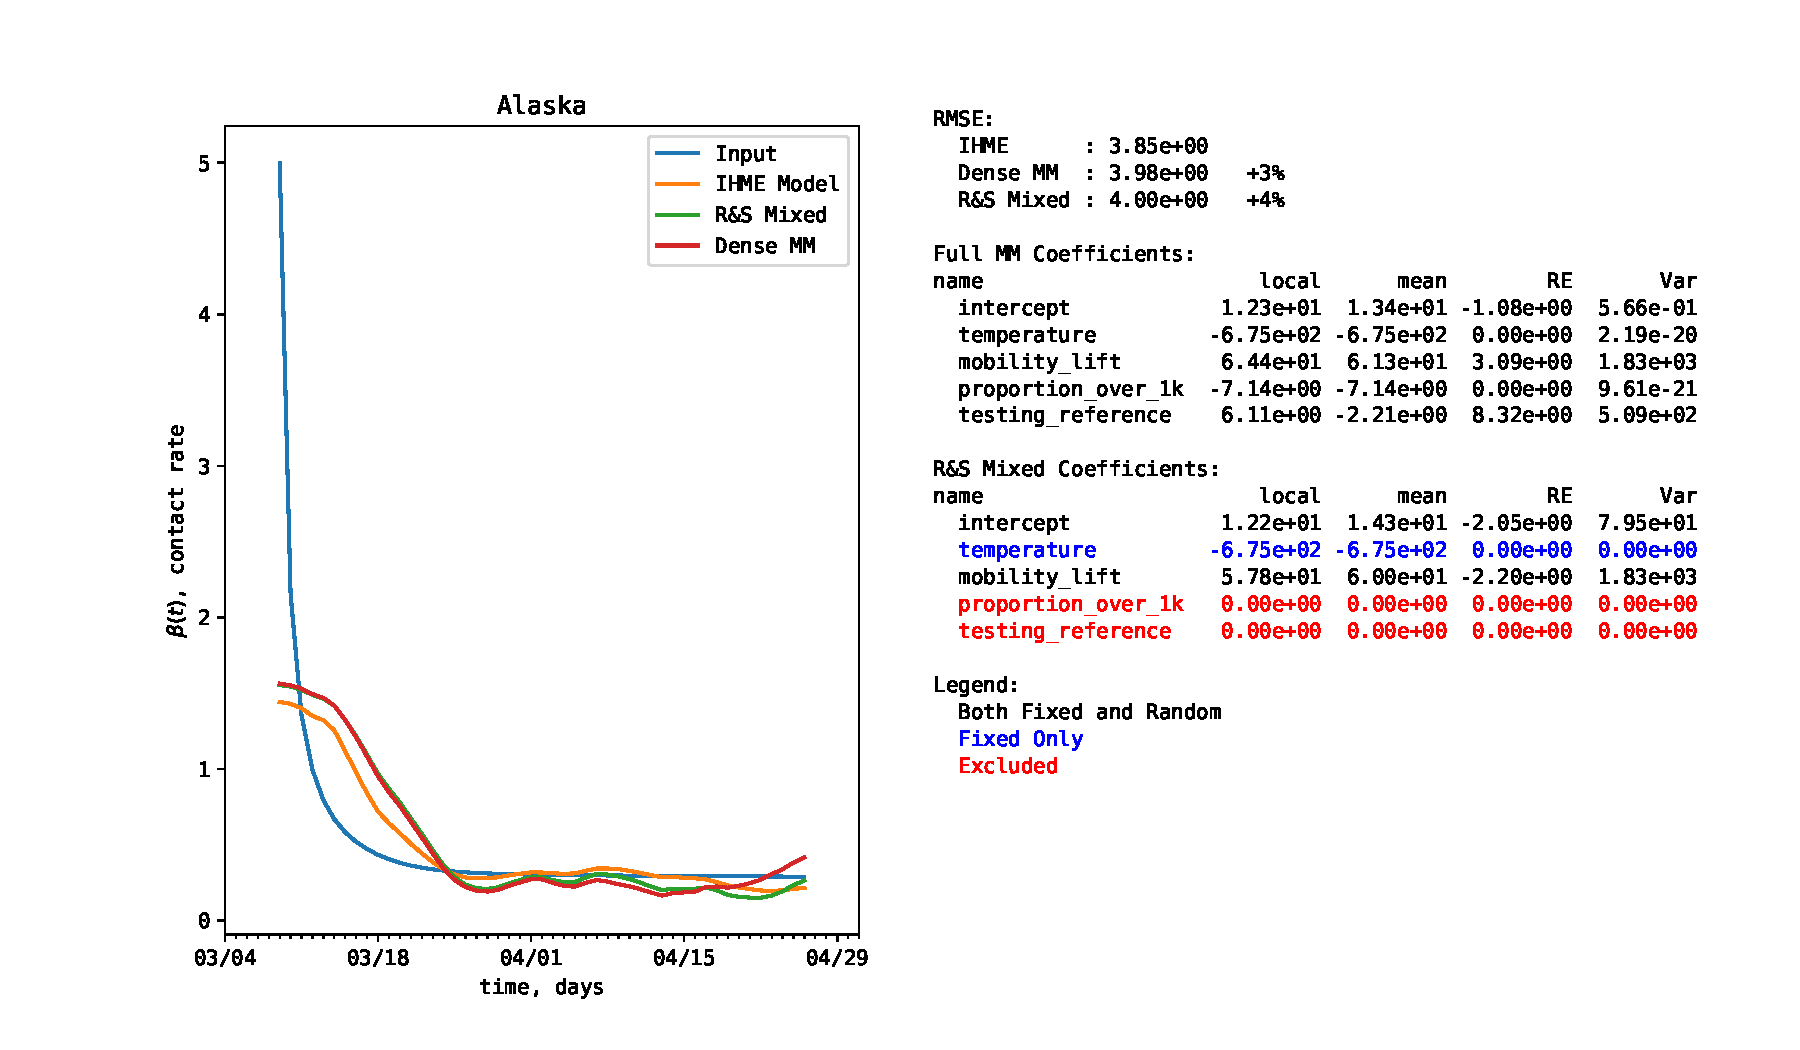
\includegraphics[width=\textwidth]{figures/fit_Alaska}
	\end{subfigure}
	\begin{subfigure}[b]{\textwidth}
		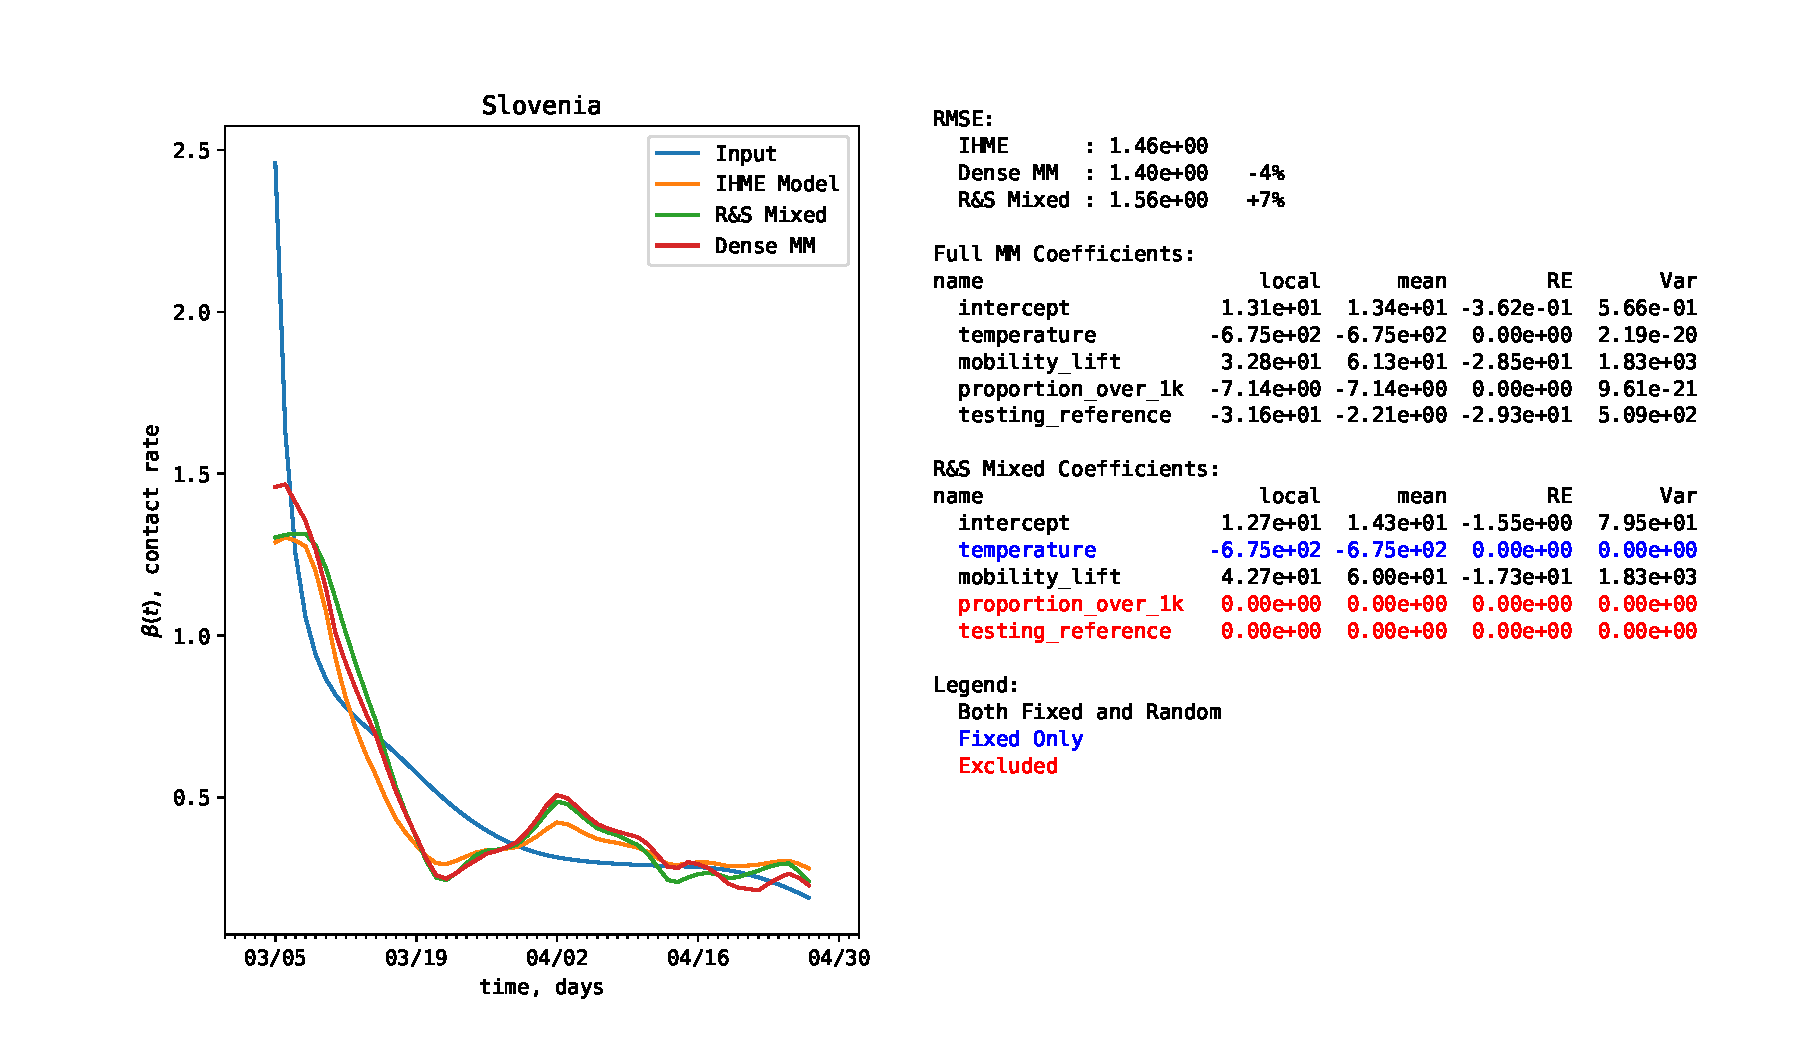
\includegraphics[width=\textwidth]{figures/fit_Slovenia}	
	\end{subfigure}
	\caption{\label{fig:covid_feature_selection_1} Comparison of fits of two different models (fully dense linear mixed model(MM) and MSR3-$\ell_0$ (R\&S) to the original IHME Projections for Alaska and Slovenia. The quality (RMSE) achieved by a sparse fit is within 10\% from a quality of both dense models which is evidences that the model picked up informative features.}
\end{figure}

\begin{figure}
	\begin{subfigure}[b]{\textwidth}
		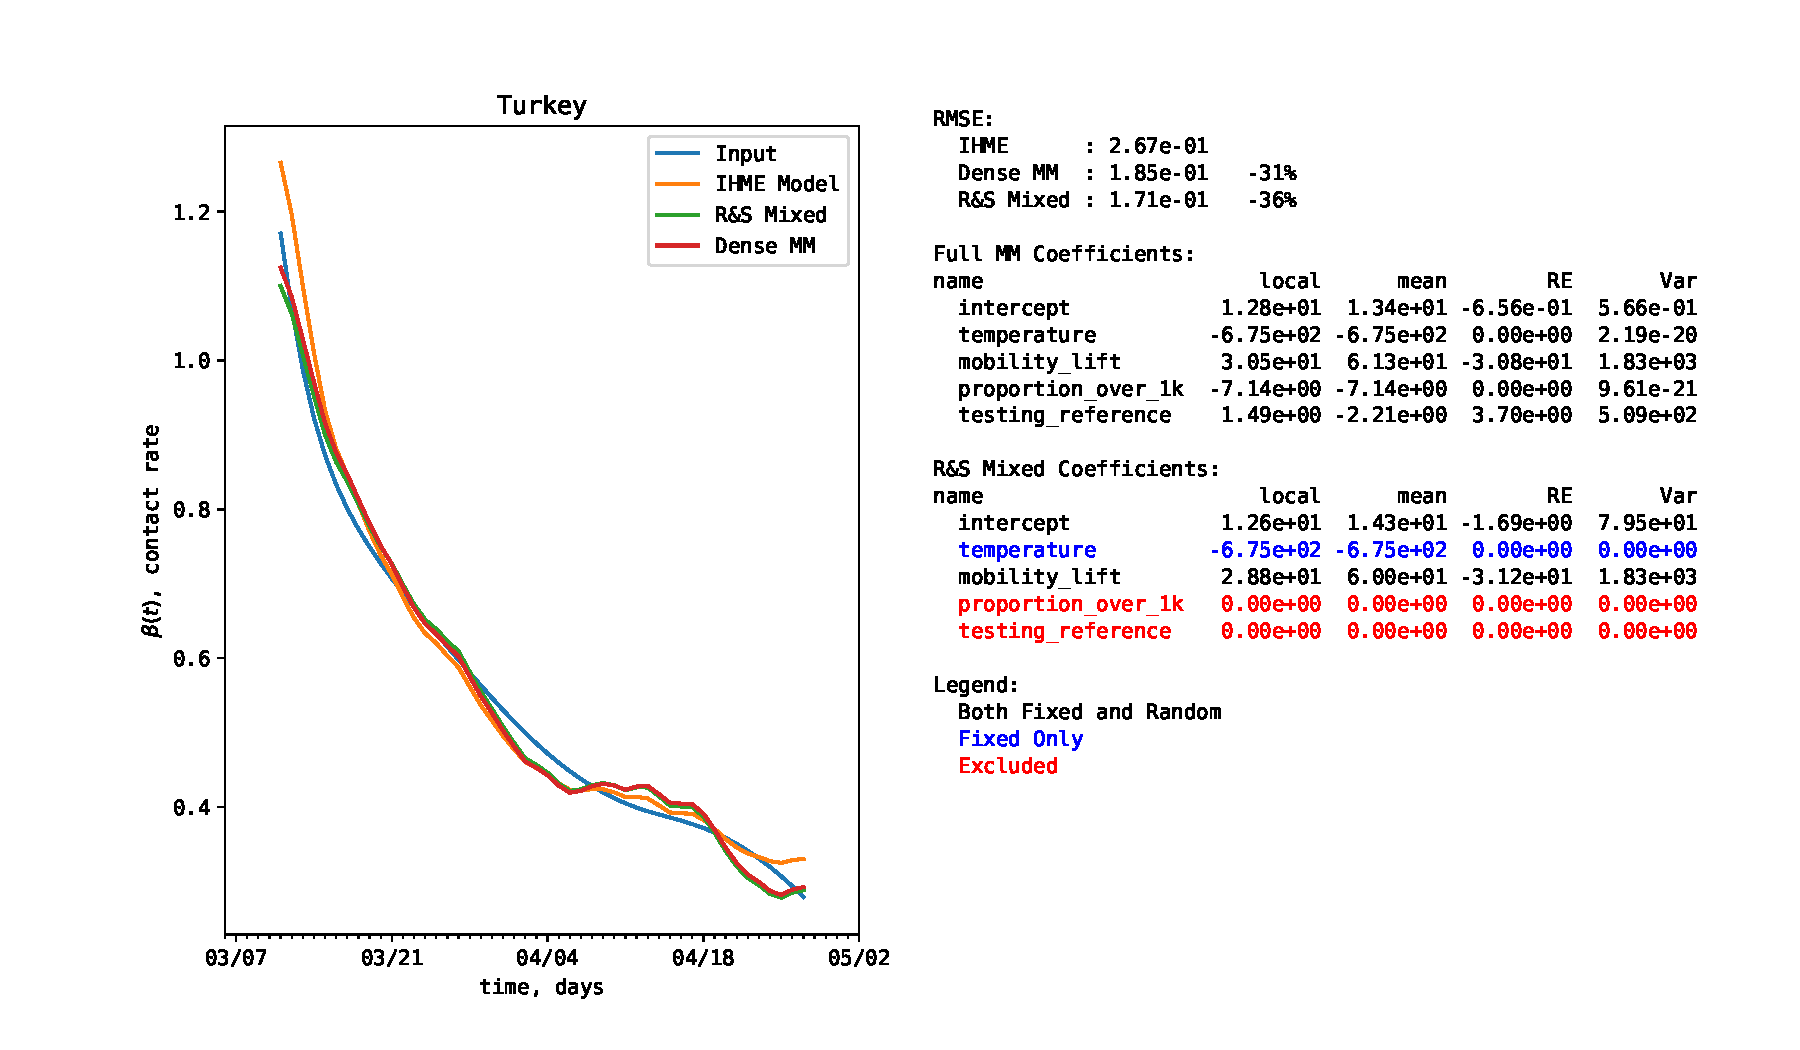
\includegraphics[width=\textwidth]{figures/fit_Turkey}
	\end{subfigure}
	\begin{subfigure}[b]{\textwidth}
		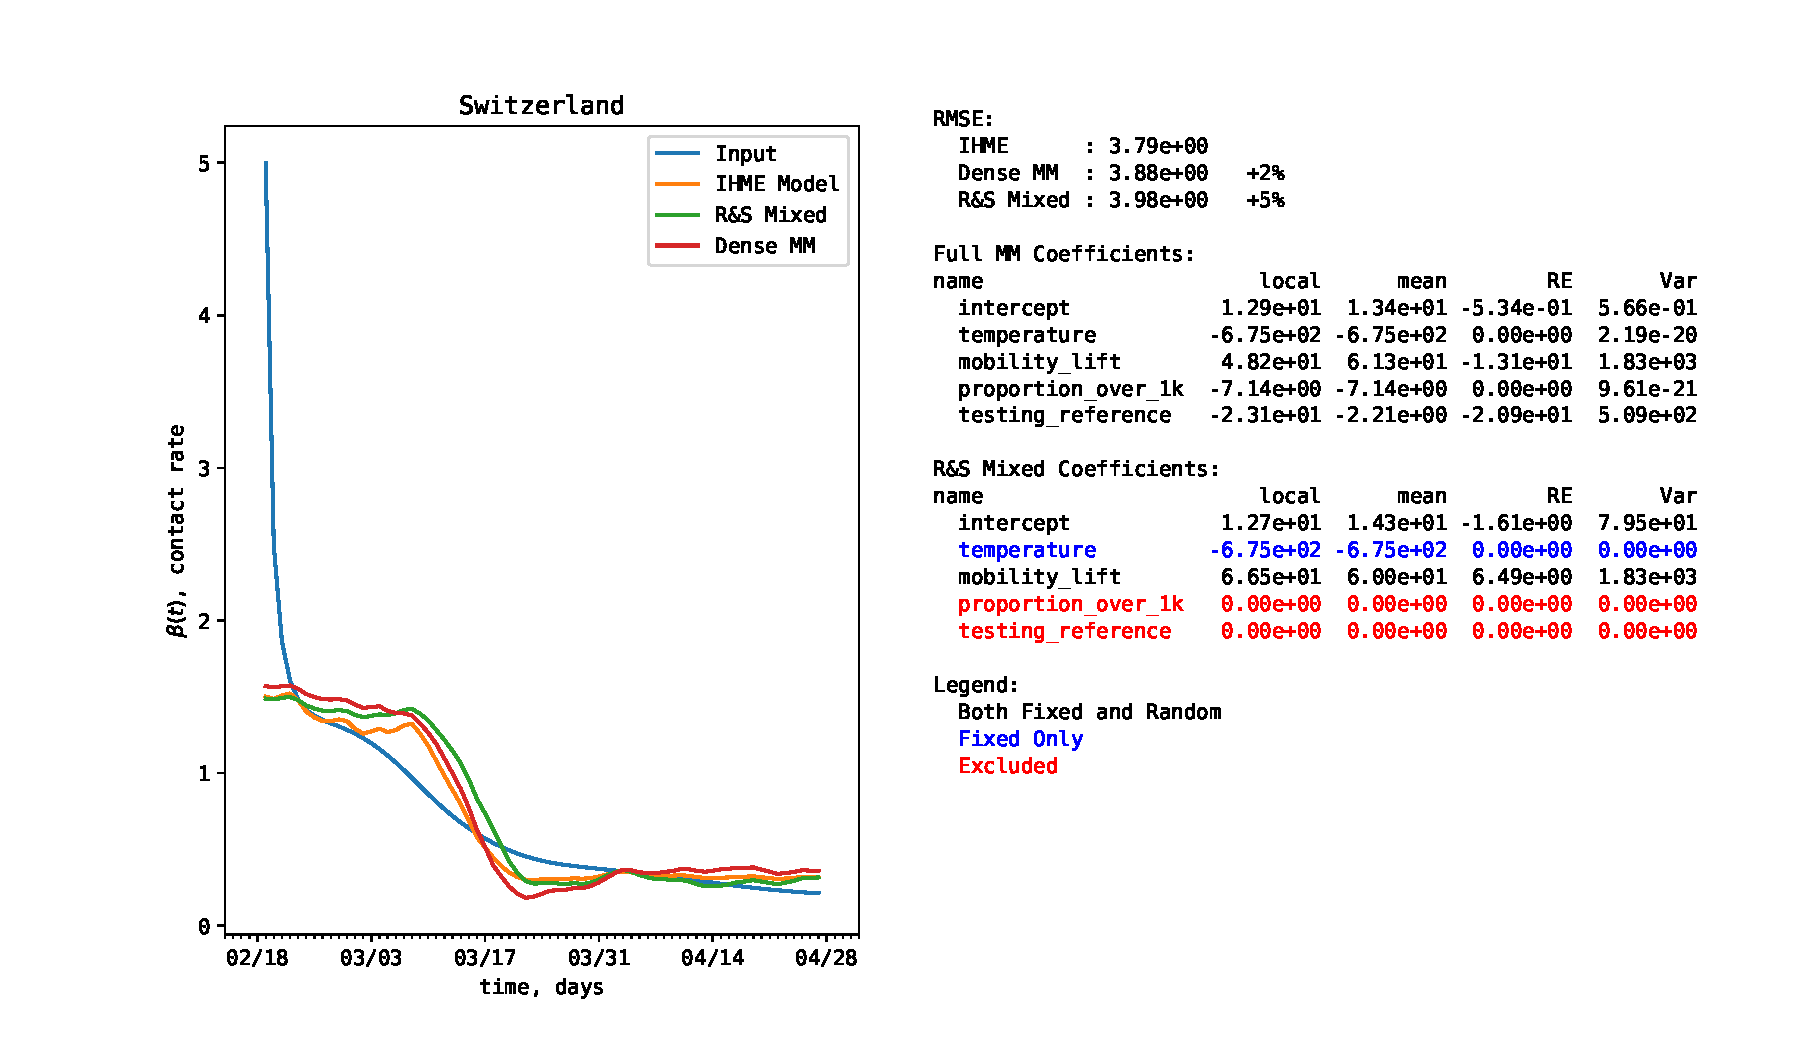
\includegraphics[width=\textwidth]{figures/fit_Switzerland}	
	\end{subfigure}
	\caption{\label{fig:covid_feature_selection_2} Comparison of fits of two different models (fully dense linear mixed model (MM) and MSR3-$\ell_0$) (R\&S) to the original IHME Projections for Turkey and Switzerland. The quality (RMSE) achieved by a sparse fit is within 10\% from a quality of both dense models which is evidences that the model picked up informative features.}
\end{figure}

In this section we apply our method to a COVID-19 Contact Rate Forecasting problem. The global pandemic created an unprecedented need for robust and accurate disease transmission forecasting. Since the beginning of the pandemic Institute for Health Metrics and Evaluation has been providing guidance to local authorities across the world with their pioneering \href{https://covid19.healthdata.org/global?view=total-deaths&tab=trend}{COVID-19 Projections tool} \cite{IHME2020Projections}. The key methodology which was essential for success in their forecasting of the disease's dynamics was transforming the death data into the contact rate time series data, and then relating this contact rate to available covariates such as temperature, social mobility, population, and others \cite{IHME2020covidnature}. All these covariates were collected in real time using limited human resources, and identifying the most important covariates was crucial for distributing these resources effectively. In the example below we show how \ouralgo can be used for making covariate selection on IHME data. 


The dataset consists of $m=60$ groups (countries or states), the detailed description of groups sizes ($n_i$) and time spans is provided in the Appendix~\ref{ch:covid}. The target variable $Y_i$ was the contact rate -- the coefficient $\beta(t)$ from an SEIR model (not to be confused with $\beta$ -- vector of fixed effects). The covariates -- columns of $X_i$ and $Z_i$ -- were: \texttt{intercept} --a column of ones,  \texttt{temperature} -- average air temperature in degrees Fahrenheit, \texttt{mobility\_lift} -- social mobility, \texttt{proportion\_over\_1k} -- population size threshold, and \texttt{testing\_reference} -- testing. The observation error's variance $\sigma_i$ was set to be 0.1.

Feature selection results for four particular locations (Alaska, Slovenia, Turkey, and Switherland) are presented on Figures \ref{fig:covid_feature_selection_1} and \ref{fig:covid_feature_selection_2}, with coefficients for the rest of the locations attached in supplementary materials. \ouralgo was charged with a task to produce a fit using only three covariates, one of which had to be mean-only (no random effects). On the left we see the original data (\texttt{Data}, in {\color{blue} blue}), and predictions of three models: IHME Projections (\texttt{IHME}, in {\color{orange} orange}), a linear mixed model fit with no selection (\texttt{Dense MM}, in {\color{red} red}), and a sparse fit of \ouralgo (\ouralgo in {\color{green} green}). The \ouralgo model has chosen to use \texttt{intercept}, \texttt{mobility\_lift}, and \texttt{temperature} covariates, with the later only as a fixed covariate; \texttt{testing\_reference} and \texttt{proportion\_over\_1k} were left out. On the plots to the left we see that the exclusion of two covariates did not significantly affect the quality of predictions. The residual errors (RMSE) to the right support this statement: the difference in RSME is within 10\% of RSME of a "dense" model which uses all the covariates, as well as from IHME's original model which fit all the locations via sequence of independent regressions. This choice also seems reasonable given the timespan: the proliferation of testing during the spring was not yet significant, so it did not inform predictions in a major way. The exclusion of \texttt{proportion\_over\_1k} could have been due to the scale of grouping: locations were grouped on the level of states and countries, not on the level of individual counties where the influence of population-based covariates could have been more significant. 

\section{Theoretical Analysis}
\label{sec:theory-paper}
%gives the problem structure used in the design of our
%numerical solution method. 
%Specifically, we design a 
%(PGD) %prox gradient 
%method 
%for solving this problem (see Section \ref{sec:pgd}). For this we must show that the function $u_\emu$
%is continuously differentiable with Lipschitz continuous gradient. 

%\section{Prox Gradient Descent}
\subsection{Proximal Gradient Descent for \texorpdfstring{$\uemu\tbg + R\tbg+\del_{\Rqp}(\tgam)$}{}} 
\label{sec:pgd}

We follow the analysis of the PGD algorithm given in \cite[Chapter 10]{AB17}
as it applies to the objective
%The application of the (PGD) %proximal gradient descent 
%algorithm to 
\begin{equation}\label{eq:varphi}
\Phi_\emu\tbg:=\uemu\tbg +\tR\tbg,\ \ \text{where}\ 
\tR\tbg:=R\tbg+\del_{\Rqp}(\tgam).
\end{equation}
%
%We now state the (PGD) %prox gradient descent 
%algorithm for finding a minimum for \eqref{eq:relax3}. 
Since $u_\emu$ is nonconvex, one typically 
applies a line search method to select stepsize. 
However, this is often not required in practice. 
For this reason we state the algorithm with and without a line search.
\medskip

%, as outlined in Algorithms \ref{alg:pgd_for_lme} and \ref{alg:MSR3}. 
%Set $\hR\tbg=R\tbg+\del_{\R^q_+}(\tgam)$ and 
%$\phi\tbg:=u_\emu\tbg+\hR\tbg$.
%See also Appendix 
%\smallskip

%\noindent
%{\bf Algorithm 1:} Proximal Gradient Descent with fixed stepsize (PGD)


%\noindent
%{\bf Algorithm 2:} Proximal Gradient Descent with Backtracking (PGD-B)

\begin{algorithm}[ht]
\SetAlgoLined
{\bf Initialize:} 
$\theta\in(0,1),\ \tau\in(0,1)$,
$\eta>0,\ \mu>0$, $\eps_{\mbox{\tiny Tol}}\ge 0$
$k=0$, $t_0>0$, $\bw^{0}=(\tbeta^0,\tgam^0)\in \Rp\times\R^q_+$
with $\inf\Phi_\emu <\Phi_\emu(\bw^0)$, 
$\gammax>\tgam^0$, 
$w^0=\prox_{t_0\tR}(\bw^{0}-t_0\nabla u_\emu(\bw^0))$.
%$, \ \eta_{Tol}\ge\eta_0>0,\ \mu_0\ge \mu_{Tol}>0$.
\\
\While{{\small $\norm{w^k-\bw^k}>\eps_{\mbox{\tiny Tol}}$
and $\gam^k\le\gammax$}}{\small\smallskip
\begin{enumerate}
\item[(i)] $t_{k+1}=\max\lset{t}{
\begin{aligned}&s\in\bW,\, t=t_0\theta^s,\ 
w=\prox_{t\tR}(w^k-t\nabla u_\emu(w^k))\\ &
\phi(w)
\le \phi(w^k)-\tau t\norm{w^k-w}^2
\end{aligned}}$.
\item[(ii)] $\bw^{k+1}=w^{k}$
\item[]$w^{k+1}=\prox_{t_{k+1}\tR}(w^k-t_{k+1}\nabla u_\emu(w^k))$
\item[]$k=k+1$
\end{enumerate}
}
\smallskip
\caption{\label{alg:pgd with bt}Proximal Gradient Descent 
fo $\Phi_\emu$ with Backtracking}
\end{algorithm}
\medskip


In Algorithm \ref{alg:MSR3}, 
the parameter $L$ is assumed to be a global Lipschitz
constant for $\nabla \uemu$. In Section \ref{sec:convergence pgd}, we show that the existence of $L$ is not needed.
In both algorithms we introduce the requirement that $\gam^k\le\gammax$.
While it is possible to include an explicit constraint of this form in the 
optimal variable selection problem \eqref{eq:lme_loss_original_in_x}, 
we do not do so since we assume that $\gammax$ is chosen 
so large that, from a practical perspective, 
the violation of this constraint indicates that the model is 
poorly posed and the algorithm needs to be terminated.
We base our analysis of the convergence properties of
Algorithms 1 and 2 on \cite[Theorem 10.15]{AB17} which makes use
of the following three basic assumptions:
\smallskip

\noindent
{\bf Basic Assumptions for the PGD Algorithm}
\begin{enumerate}
\item[(A)] $\map{\tR}{\Rp\times\Rq}{\eR}$ is a closed proper convex function.
\item[(B)] $\map{\uemu}{\Rp\times\Rq}{\eR}$ is closed and proper, 
$\dom{\uemu}$ is
convex, $\dom{\tR}\subset\intr{\dom{\uemu}}$, and
$\uemu$ is $L_\emu$-smooth over $\intr{\dom{\uemu}}$.
\item[(C)] Problem \eqref{eq:relax3} has an optimal solution with optimal 
value $\Phi_{\mbox{\tiny OPT}}$.
\end{enumerate}

\noindent
We assume that (A) holds. This is not an overly
restrictive assumption since it is satisfied by most of the standard
variable selection regularizers.
We show that (C) holds when $R$ satisfies
an additional coercivity hypothesis (Theorem \ref{thm:relaxed existence}). 
On the other hand, establishing that (B) holds
in a concrete setting such as ours
can be quite difficult. 
In particular, just as with $\LL$, $\uemu$ may fail to be globally Lipschitz.
Validating Assumption (B) as well as developing a technique for circumventing
the need for a global Lipschitz constant for $\nabla\uemu$ 
consumes the majority of the theoretical development. 
%Assumption (B) is particularly difficult since $\uemu$ is an optimal value function.
%We establish $B$ established in several steps.
%However, we show that the global Lipschitz continuity of $\nabla \uemu$
%is not required in practice for the theory developed in 
%\cite{AB17} to apply. 
%We begin by establishing the smoothness of $\uemu$.

%\begin{figure}[ht]
%    \centering
%    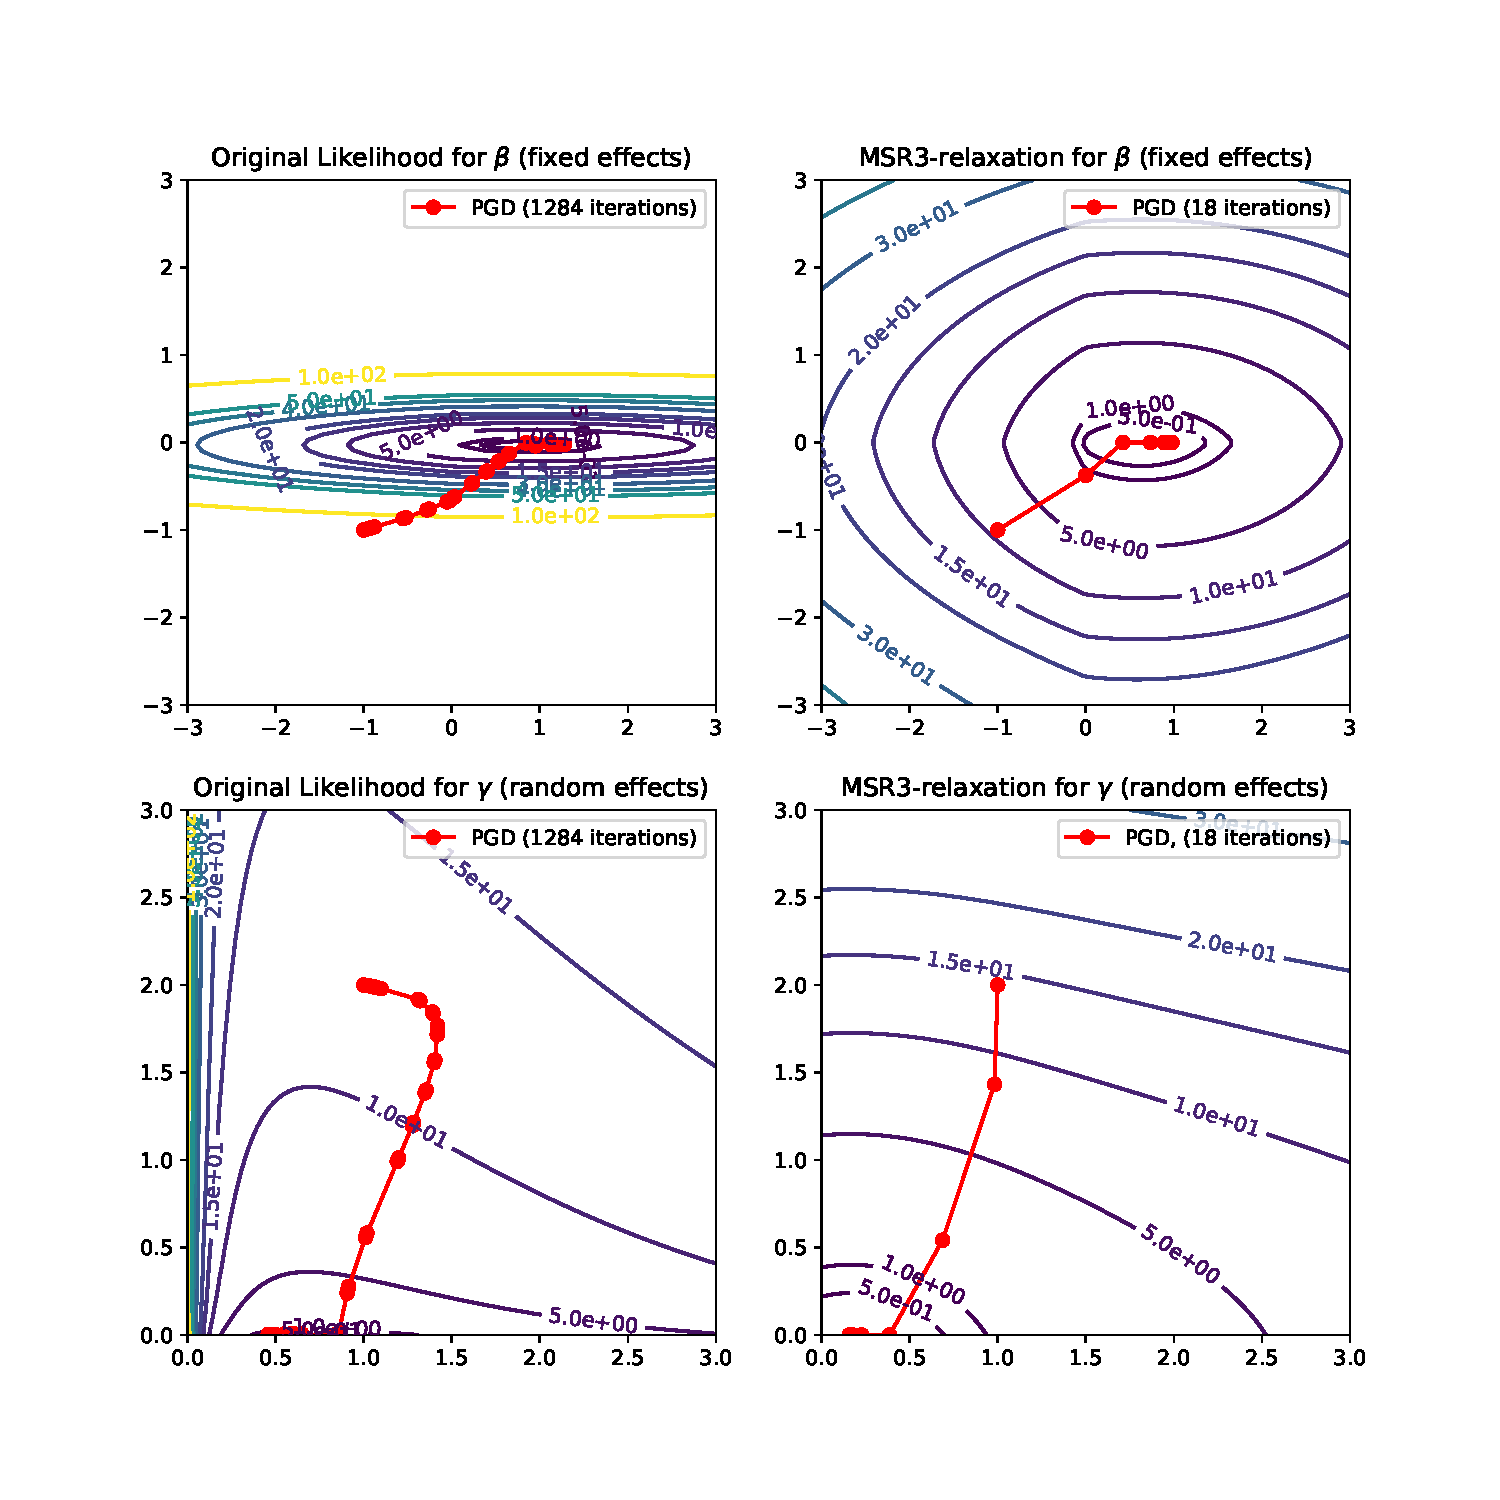
\includegraphics[width=\textwidth]{Images/intuition_current.pdf}
%    \caption{Proximal Gradient Descent (PGD) takes an order of magnitude fewer iterations to converge when optimizing a value function instead of the original likelihood, because SR3-relaxation improves the conditioning of the problem, which results in a more spherical level-sets. This effect persists for both quadratic convex (first row) and non-convex components (second row) of the likelihood. The effect is stronger for  minima near the boundary of the constraint region 
%    (bottom-left panel).}
%    \label{fig:geometric_intuition_sr3}
%\end{figure}


\subsection{The Smoothness of \texorpdfstring{$u_\emu$}{}}\label{sec:smoothness}
We investigate the relationship between the problems \eqref{eq:lme_loss_original_in_x}
and \eqref{eq:relax2}, the existence of solutions to 
 \eqref{eq:relax2}, and the properties of the function $\uemu$ and its derivative.
%We begin with an examination of the function $\LL$
%and 
%The first step is to understand the role of the parameter $\blam$.

\subsubsection{Underlying convexity}

\begin{lemma}[$\LL+\phimu$ is Weakly Convex]\label{lem:LL weak cvx}
Let $\LL$ be as given in \eqref{eq:lme_diagonal_setup}. Then
\begin{equation}\label{eq:hess LL}
\nabla^2\LL{(\beta,\gam)}=\sum_{i=1}^m
S_i^T\begin{bmatrix}X_i^T\\ -Z_i^T\end{bmatrix}
\Omega_i(\gam)^{-1}
\begin{bmatrix}X_i& -Z_i\end{bmatrix}S_i
-\begin{bmatrix}
0&0\\ 0& \half(Z_i^T\Omega_i(\gam)^{-1}Z_i)^{\circ2}
\end{bmatrix},
\end{equation}
for all
$(\beta,\gam)\in\R^p\times\R^q_+$, where 
\[
S_i:=\begin{bmatrix}
I_q&0\\ 0&\Diag{Z_i^T\Omega_i^{-1}(X_i\beta-Y_i)}
\end{bmatrix}
\]
and, for any $A\in\R^{t\times t}$, $A^{\circ 2}:=A\circ A$. In particular, this implies
that the matrix
\begin{equation}\label{eq:psd for LL}
\begin{bmatrix}
\nabla_{\beta\beta}\LL(\beta,\gam)&\nabla_{\gam\beta}\LL(\beta,\gam)\\
\nabla_{\beta\gam}\LL(\beta,\gam)&\nabla_{\gam\gam}\LL(\beta,\gam)
+\blam I\end{bmatrix}
\end{equation}
is positive semidefinite
for $\bar\eta= \nu m$, where
\[
\nu:=max\lset{(1/2) \mu_\mmin(\Lam_i)^{-2}\sig^4_\mmax(Z_i)}{i=1,\dots,m},
\]
$\mu_\mmin(\Lam_i)$ is the smallest eigenvalue of $\Lam_i$, and
 $\sig_\mmax(Z_i)$ is the largest singular value of $Z_i,\, i=1,\dots,m$.
Consequently, for any $\tbg\in\dom{\tR}$ and $\mu\ge 0$, the mapping 
\(
\bg\mapsto \LL_{\emu}(\bg, \tbg)
%\hLL(\bg,\tgam) %:=\LL(\beta,\gam)+\frac{\blam}{2}\norm{\gam-\hgam}^2
%\sum_{i=1}^m\frac{\nu_i}{2}\norm{\gam-\hat\gam}^2,
\)
is convex for all $\eta\ge\bar\eta:=\nu m$.
In particular, this implies that $\LL+\phimu$ is weakly convex for any $\mu\ge 0$, 
and the mapping
\(
%\begin{aligned}
\bg\mapsto\LL_{\emu}(\bg,\tbg)
%&=
%\LL\bg+\phimu(\gam)+
%\keta(\beta-\tbeta,\beta-\tbeta)
%\\ &=
%\hLL(\bg,\tgam)+    \frac{\eta}{2}\norm{\bg-\tbg}^2 
%\end{aligned}
\)
is strongly convex for $\eta> \bar\eta$ with modulus of strong convexity $(\eta-\bar\eta)$
regardless of the choice of $\tbg\in\Rp\times\Rq$.
%Moreover, the mapping 
%\eq{\label{eq:defn L sub eta}
%(\beta, \gamma)\mapsto    
%\LL_{\eta}(x, w) := \tLL(x, w) + \frac{\eta}{2}\norm{x-w}^2 
%}
%is strongly convex for every $\eta>0$ and any choice of 
%$(\tbeta,\tgam)\in\R^p\times\R^q$.
\end{lemma}
\begin{proof}
The formula for $\nabla^2\LL$ is given in Appendix \ref{appendix:derivatives_of_lmm}
(see \eqref{eq:hess LL}).
By \cite[Theorem 3.1]{ABBP2021}, 
$\mu_\mmax(\left(Z_i^T\Omega_i(\gam)^{-1}Z\right)\le
\lam_\mmin^{-1}\sig_\mmax^2(Z_i)$, and since 
$\mu_\mmax(H^{\circ 2})\le \mu_\mmax^2(H)$
for all $H\in\bS^q_+$ \cite{HJ85}, we have
\[
\mu_\mmax\left(\half(Z_i^T\Omega_i(\gam)^{-1}Z_i)^{\circ2}\right)
\le (1/2) \lam_\mmin^{-2}
\sig^4_\mmax(Z_i)=:\nu_i
\qquad  i=1,\dots,m.
\]
This establishes that the matrix in \eqref{eq:psd for LL} is positive semidefinite.
Since $\phimu$ is convex, the mapping
\[
(\beta,\gam)\mapsto \LL_{\emu}(\bg,\tbg) %\hLL((\beta,\gam),\tgam)
\]
is strongly convex for any choice
of $\blam> \nu m$, where 
\eq{\label{eq:nu}
\nu:=\max_{i=1,\dots,m}\nu_i.
}
%The strong convexity statement follows from 
%the fact that
%$\nabla^2 \LL_{\eta}((\beta, \gamma), (\tbeta, \tgamma))
%=\nabla^2 \LL(\beta,\gam)+\eta I$ where $\nabla^2 \tLL(\beta,\gam)$
%is positive semidfinite.
\end{proof}
For the remainder of the paper, we assume that 
\eq{\label{eq:blam1}\eta> \nu m=:\bar\eta} 
so that the mapping
$(\beta,\gam)\mapsto \LL_{\emu}(\bg,\tbg)$ %\hLL((\beta,\gam),\tgam)$
is strongly convex with 
%$\nabla_{\bg\bg}^2\hLL(\bg,\tgam)$ 
positive definite Hessian
regardless of the 
choice of $\tgam\in\R^q$. With this in mind, the function $\uemu$ defined by
\eqref{eq:value_function_definition} resembles a Moreau envelope.
%of the convex function $\hLL+\phi_\mu$.
However, this is misleading since, in particular,
we are not even assured of the existence of solutions to
the optimization problem defining $\uemu$. 

\subsubsection{Existence and consistency}\label{ssec:existence and consistency}

To establish the existence of solutions to the relaxed
optimization problems \eqref{eq:relax2} and the
problems defining the parametrized family $\uemu$ in
\eqref{eq:value_function_definition}, we assume that $R$ is $1$-coercive.
\begin{lemma}\label{lem:lb plus 1c}
Given $\mu>0$ let $\phimu$ be as defined above, and assume that 
$\map{R}{\Rp\times\Rq}{\R\cup\{+\infty\}}$
is 1-coercive, i.e., 
\(
\liminf_{\Vert{\tbg}\Vert\rightarrow\infty}\Vert{\tbg}\Vert^{-1}R\tbg>0.
\)
Then 
%the objective function in \eqref{eq:relax},
$\phimu+R$ 
%\(
%\wLL_\emu(\bg,\tbg):=\LL_{\emu}(\bg, \tbg)+R\tbg+\del_{R^q_+}(\tgam)
%\),
is level compact.
\end{lemma}
%\begin{proof}
%By Lemma \ref{lem:LL weak cvx}, for every $\tbg \in\Rp\times\Rq$,
%the mapping 
%$\bg\mapsto \LL_{\emu}(\bg, \tbg)$
%is strongly convex with modulus of strong convexity $\eta$.
%Consequently, for every $\tbg \in\Rp\times\Rq$,
%\[
%\begin{aligned}
%\LL_{\emu}((0,\one),\tbg)&+
%\ip{\nabla_{\bg}\LL_{\emu}((0,\one),\tbg)}{\bg-(0,\one)}+
%\frac{\eta}{2}\norm{\bg-(0,\one)}^2
%\\
%&\le \LL_{\emu}(\bg, \tbg)
%\qquad\forall\, \bg\in\Rp\times\R^q_{++},
%\end{aligned}
%\]
%which implies that
%\[\begin{aligned}
%&\LL(0,\one)+q\mu\ln(\mu)+\kappa_\eta(\tbeta,\tgam-\one)
%-\norm{\nabla_\beta \LL(0,\one)}\norm{\beta}-
%\norm{\nabla_\gam \LL(0,\one)}\norm{\gam-\one}-\mu^2\sqrt{q}\norm{\gam-\one}
%\\ &
%-\eta\ip{\tbeta}{\beta}+(\blam+\eta)\ip{\one-\tgam}{\gam-\one}
%+\frac{\eta}{2}\norm{(\beta,\gam)-(0,\one)}^2
%\\ &
%\le \LL_{\emu}(\bg, \tbg)
%\qquad\qquad\forall\, \bg\in\Rp\times\R^q_{++}.
%\end{aligned}
%\]
%That is, there are constants $\xi_0\in\R,\ \xi_1,\xi_2,\xi_3,\xi_4>0$ such that
%\[
%\begin{aligned}
%\xi_0+(\xi_2\norm{\beta}^2-\xi_1\norm{\beta})
%+(\xi_4\norm{\gam-1}^2-\xi_3\norm{\gam-\one})
%-\eta\ip{\tbeta}{\beta-\tbeta}-(\blam+\eta)\ip{\one-\tgam}{\gam-\one}
%\\ 
%\leq\LL_{\emu}(\bg, \tbg)
%\quad\forall\, \bg\in\Rp\times\R^q_{++}.
%\end{aligned}
%\]
%\end{proof}
%
\begin{proof}
If $\mu=0$, then the result is trivially true, so we assume that $\mu>0$.
Let $\{\bgk\}\subset \Rp\times\Rqp$ be such that $\norm{\bgk}\uparrow\infty$.
We need to show that $\phimu(\gam^k)+R\bgk\rightarrow \infty$.
If $\{\gam^k\}$ is bounded, then $\phimu(\gam^k)+R\bgk\rightarrow \infty$
since in this case $\phimu(\gam^k)$ is bounded below.
So assume that $\{\gam^k\}$ is unbounded which implies that
$\phimu(\gam^k)\rightarrow -\infty$. Since $R$ is 1-coercive,
we know that there is an $\hat\alf>0$ such that, for $k$ sufficiently large,
$R\bgk\ge\hat\alf\sum_{i=1}^q\gam^k_i$. But then
$\phimu(\gam^k)+R\bgk\ge \sum_{i=1}^q(\hat\alf\gam^k_i-\mu\ln(\gam^k_i))$
where the right-hand side diverges to $+\infty$ as $k\uparrow\infty$.
Hence, $\phimu(\gam^k)+R\bgk\rightarrow \infty$.
\end{proof}

%We have the following result concerning the existence of solutions to
%\eqref{eq:relax2}.


\begin{theorem}\label{thm:relaxed existence}
Let $\LL$  be as in Theorem \ref{thm:basic existence2}
and let $\eta> 0$ satisfy \eqref{eq:blam1}.
Let $\mu\ge 0$. If $\mu=0$, assume that $\map{R}{\Rp\times\Rq}{\R_+\cup\{+\infty\}}$
is level compact; otherwise, assume $R$
is 1-coercive.
%Then, for every $\tgam\in\Rq$, there exists 
%$(\beta^*_\tgam,\gam^*_\tgam)\in\Rp\times\Rqp$
%such that 
%\[
%\LL(\beta^*_\tgam,\gam^*_\tgam)+\phimu(\gam^*_\tgam)
%\le \LL_{\emu}(\bg,\tbg)\quad\forall\ (\bg,\tbg)\in(\Rp\times\Rqp)\times(\Rp\times\Rq).
%\]
%In addition, suppose $R$ satisfies
%\eq{\label{eq:R condition}
%\left[\eta>0\, \text{and}\ \Xi(\eta,\rho)\!:=\!\lset{(x,w)\in\CC\times\CC}{\LL_\eta(x,w)\le \rho}\ne\emptyset
%\right]\implies 
%\emptyset\ne\argmin_{(x,w)\in \Xi(\eta,\rho)}R(w).
%}
%Furthermore, 
%if $R$ is level compact, t
Then solutions to \eqref{eq:relax2} always exist.
\end{theorem}
\begin{proof}
Let 
\(
v^* %\!:=\!\inf\!\lset{\!\LL_\emu(\bg,\tbg)\!+\!R\tbg\!}{\!0\!\le\!\tgam\!}
\)
be the optimal value in \eqref{eq:relax2}
and let
\(
\!\{(\bgk,\tbgk)\}\!\subset (\Rp\times\Rqp)^2
\) 
be such that
\(
\LL_\emu(\bgk,\tbgk)\!+\!R\tbgk\downarrow v^*\!.
\)
By \eqref{eq:eigbd} and \eqref{eq:eig1}, 
it must be the case that 
\begin{equation}\label{eq:lower bd}
%\max\{\ln(\norm{r(\beta^k}^2/n),\ln\norm{\hOmega(\gam^k)}\} + 
\begin{aligned}
\LL_\emu&(\bgk, \tbgk)+R\tbgk
\\ &\ge
\frac{n\!+\!1}{2}\ln(\talf)+\phimu(\gam^k)+
\keta(\beta^k-\tbeta^k,\gam^k-\tgam^k)+R\tbgk
\\ &\ge
\frac{n\!+\!1}{2}\ln(\talf)+\phimu(\gam^k)+\frac{\bar\eta}{2}\norm{\gam^k-\tgam^k}^2
+R\tbgk.
\end{aligned}
\end{equation}
%where $\bar\eta:=\nu m$.


If $v^*=-\infty$, then \eqref{eq:lower bd} tells us that
\begin{equation}\label{eq:minus infty1}
%\max\{\ln(\norm{r(\beta^k}^2/n),\ln\norm{\hOmega(\gam^k)}\} + 
\phimu(\gam^k)
+\frac{\blam}{2}\norm{\gam^k-\tgam^k}^2+R\tbgk\rightarrow-\infty.
\end{equation}
This in turn implies that $\mu>0$, $\phimu(\gam^k)\rightarrow-\infty$
and $\norm{\gam^k}\rightarrow \infty$.
Since $R$ is 1-coercive and $\norm{\gam^k}\rightarrow \infty$, 
we can assume with no loss in generality that there is an $\balf>0$
such that $R\tbgk\ge \balf \sum_{i=1}^q\tgam^k_i$ for all $k\in\N$. 
Consequently,
\eq{\label{eq:unbdd1}\begin{aligned}
\phimu(\gam^k)
+&\frac{\blam}{2}\norm{\gam^k-\tgam^k}^2+R\tbgk
\\ &\ge
\sum_{i=1}^q\left(-\mu\ln (\gam^k_i/\mu)+\frac{\blam}{2}(\gam^k_i-\tgam^k_i)^2
+\balf\tgam^k_i\right)
\\ &= 
\sum_{i=1}^q\left(
(-\mu\ln (\gam^k_i/\mu)+\balf\gam^k_i)+\frac{\blam}{2}(\gam^k_i-\tgam^k_i)^2
-\balf (\gam^k_i-\tgam^k_i)
\right)
\\ &=
\sum_{i=1}^q\left(
(-\mu\ln (\gam^k_i/\mu)+\balf\gam^k_i)+\frac{\blam}{2}
\left[(\gam^k_i-\tgam^k_i-\frac{\balf}{\blam})^2-(\frac{\balf}{\blam})^2\right]
\right)
\\ &\ge -q\frac{\balf^2}{2\blam}+\sum_{i=1}^q
(-\mu\ln(\gam^k_i/\mu)+\balf\gam^k_i)
\\ &= -q\frac{\balf^2}{2\blam}+\phimu(\gam^k)+\balf\norm{\gam^k}_1\ 
\rightarrow +\infty,
\end{aligned}}
which is a contradiction. Hence $v^*>-\infty$.

Let $\rho> v^*>-\infty$. If $\{\gam^k\}\subset\Rqp$ is unbounded, we may assume with no
loss in generality that $\norm{\gam^k}\rightarrow+\infty$. 
If $\mu=0$, then, by  \eqref{eq:lower bd},
\(
\rho>\frac{n\!+\!1}{2}\ln(\talf)+R\tbgk
\uparrow +\infty,
\)
a contradiction, and so we can assume that $\mu>0$ and $R$ is 1-coercive.
%Lemma \ref{lem:lb plus 1c} tells us that
%$\phimu+R$ is coercive.
Using \eqref{eq:lower bd} we may proceed as in \eqref{eq:unbdd1} to find that
\begin{equation}\label{eq:lbd2}
%\begin{aligned}
\rho > \frac{n\!+\!1}{2}\ln(\talf)
-q\frac{\balf^2}{2\blam}+\sum_{i=1}^q
(-\mu\ln \gam^k_i+\balf\gam^k_i)\ 
\rightarrow +\infty,
\end{equation}
again a contradiction, so the sequence $\{\gam^k\}$ is bounded.
Therefore, the first inequality in \eqref{eq:lower bd} tells us that the entire sequence 
$\{(\bgk,\tbgk)\}$ is necessarily bounded.
Consequently, a limit point of the sequence $\{(\bgk,\tbgk)\}$ exists and,
since $R$ is lsc, any such
limit point is a solution to 
\eqref{eq:relax2}.
\end{proof}

%
%\begin{proof}
%The proof follows the pattern given for Theorem \ref{thm:basic existence}.
%Since 
%Let $\map{A}{(\R^p\times\R^q)\times(\R^p\times\R^q)}
%{\R^n\times\bS^n\times(\R^p\times\R^q)\times(\R^p\times\R^q)}$ be the affine transformation 
%\[
%A((\beta,\gam),(\tbeta,\tgam))=
%(r(\beta),\hOmega(\gam),(\beta-\tbeta,\gam-\tgam),(\tbeta,\tgam)),
%\]
%and let $\map{\hf}{\R^n\times\bS^n_{++}\times(\R^p\times\R^q)\times(\R^p\times\R^q)}{\R}$ be defined by
%\[
%\hf(r,M,(y,z),(\tbeta,\tgam)):=f(r,M)+ \phimu(\gam)+
%\kappa_\eta(y,z) %\frac{\eta}{2}\norm{y}^2 + \frac{\blam+\eta}{2}\norm{z}^2 
%+R(\tbeta,\tgam).   
%\]
%%where $\map{\kappa_\eta}{\R^p\times\R^q}{\R}$ is the coercive mapping
%%\begin{equation}\label{eq:kappa}
%%\kappa_\eta(y,z):=\frac{\eta}{2}\norm{y}^2 + \frac{\blam+\eta}{2}\norm{z}^2.
%%\end{equation}
%Then
%\[
%\LL_{\emu}((\beta,\gam),(\tbeta,\tgam)) + R(\tbeta,\tgam)
%=\hf(A((\beta,\gam),(\tbeta,\tgam))).
%\]
%Let 
%\(
%\rho>v^*:=\inf\lset{\LL_\emu(\bg,\tbg)+R\tbg}{0\le\tgam}
%\) 
%and set
%\(
%\MM_\rho:=\lev{\LL_\eta+R}{\rho}\cap(\Rp\times\Rq\times\Rp\times\R^q_+).
%%\lset{(x,w)\in\CC\times\CC}{\LL_\eta(x,w)+R(w)\le \rho}.
%\)
%Since $\LL(x)\le \LL_\eta(x,w)\le \rho$, $\kappa_\eta(y,z)\le\rho$ and
%$R(w)\le\rho$ for every $(x,w)\in\MM_\rho$,
%\[
%\FF:=
%\lset{A(x,w)}{(x,w)\in\CC^2\cap\MM_\rho}\subset\hDD_{\rho\talf\eta}:=
%\DD_{\rho\talf}\times\lev{f}{\rho}\times\lev{R}{\rho},
%%\lset{(r(\beta),\hOmega(\gam)}}{\exists\, w\in\CC\ \text{s.t.}\ 
%%((\beta,\gam),w)\in\MM_\rho}\subset\DD_{\rho\talf},
%\]
%where $\talf:=\mu_\mmin(\Lam)$ and 
%$\hDD_{\rho\talf\eta}$ is compact by
%Theorem \ref{lem:levelcompact1} and our coercivity assumption on $R$. 
%By taking $R\equiv0$ in
%Corollary \ref{cor:basic existence}, there exists $x^*\in\CC$ %$x^*=(\beta^*,\gam^*)$
%such that $\LL(x^*)=\min_{x\in\CC}\LL(x)$, and so $\LL(x^*)\le v^*$. 
%Let $\{(x^k,w^k)\}\subset\CC^2$ be such that 
%$\LL_{\eta}(x^k,w^k) + R(w^k)\downarrow v^*$.  
%Since $\{A(x^k,w^k)\}\subset\hDD_{\rho\talf\eta}$, we may assume with no loss in 
%generality that $A(x^k,w^k)\rightarrow(\br,\bOmega,(\by,\bz),\hw)$
%for some 
%$(\br,\bOmega,(\by,\bz),\hw)\in(\R^n\times\bS_+^n\times(\R^p\times\R^q)^2)
%\cap\im{A}$. Since $(\tbeta^k,\tgam^k)=w^k\rightarrow\hw=(\hat\beta,\hat\gam)$,
%we have $(\beta^k,\gam^k)\rightarrow(\by+\hat\beta,\bz+\hat\gam)
%=:(\bar\beta,\bar\gam)$ and
%$(r(\beta^k),\hOmega(\gam^k))\rightarrow
%(r(\bar\beta),\hOmega(\bar\gam))$. Therefore, 
%$\LL_{\eta}((\bar\beta,\bar\gam),(\hat\beta,\hat\gam)) + R(\hat\beta,\hat\gam)
%=v^*$ since $\LL_\eta+R$ is continuous on $\MM_\rho$.
%\end{proof}

Next we fix $\mu\ge 0$ and show that as 
$\eta\uparrow\infty$ the solutions to 
\eqref{eq:relax2} converge to solutions of
\begin{equation}\label{eq:log-barrier problem}
\min_{\bg\in\CC}\LL\bg+\phimu(\gam)+R\bg.
\end{equation}
In particular, for $\mu=0$, they converge to solutions of 
\eqref{eq:lme_loss_original_in_x}.

\begin{theorem}[Consistency as $\eta\rightarrow\infty$]\label{thm:eta consistency}
Let $\LL$ and $R$ be as in Theorem \ref{thm:relaxed existence}
and fix $\mu\ge 0$.
Let $\{\eta_k\}\subset\R_{++}$ be such that $\eta_k<\eta_{k+1}$
with $\eta_k\uparrow\infty$, and let $(\bgk,\tbgk)$ be an optimal solution to 
\eqref{eq:relax2} for $(\emu)=(\eta_k,\mu)$, $k\in\N$.
Then any limit point (equivalently, cluster point) 
$(\bbg,\hbg)$ of $\{(\bgk,\tbgk)\}$ satisfies
$\bbg=\hbg$ with $\bbg$ being an optimal solution to 
\eqref{eq:log-barrier problem}.
\end{theorem}
\begin{proof}
With no loss in generality $\eta_k>\bar\eta$ for all $k$.
Set 
\[\left.\begin{aligned}
a_k(x,w)&:=\LL_{\eta_k,\mu}(x,w)+R(w)\\ 
b_k(x,w)&:=\LL(x)+\phimu(\gam)+R(w)\\
c_k(x,w)&:=\kappa_{\eta_k}(\beta-\tbeta,\gam-\tgam)
\end{aligned}\right\}\quad \forall k\in\N,
\] 
where 
$x=(\beta,\gam)$ and $w=(\tbeta,\tgam)$ with $\kappa_\eta$ defined in
\eqref{eq:kappa}. Set $x^k=\bgk,\ \bx=\bbg,\ w^k=\tbgk$ and $\hw=\hbg$.
By Lemma \ref{lem:lb plus 1c} and Theorem \ref{thm:basic existence2} 
with $\hR=\phimu+R$, 
%\ref{thm:relaxed existence}, 
there is an optimal solution $\xmu$ 
to \eqref{eq:log-barrier problem} %\eqref{eq:lme_loss_original_in_x} 
yielding an optimal value of $\vmu$ for which 
$a_k(x^k,w^k)\le a_k(\xmu,\xmu)=\vmu$ for all $k\in\N$. Hence, the sequence
$\{a_k(x^k,w^k)\}$ is upper bounded by $\vmu$.
Since
\[
a_k(x^k,w^k)\le a_k(x^{k+1},w^{k+1})\le a_{k+1}(x^{k+1},w^{k+1}),
\]
there exists $\tv$ such that
$a_k(x^k,w^k)\uparrow\tv\le \vmu$.
Next, observe that
\[
a_k(x^k,w^k) \le a_k(x^{k+1},w^{k+1})\ \ \text{ and }\ \ 
a_{k+1}(x^{k+1},w^{k+1})\le a_{k+1}(x^{k},w^{k}).
\]
By adding these inequalities together we find that 
$\norm{x^{k+1}-w^{k+1}}\le \norm{x^{k}-w^{k}}$ so that 
$\norm{x^{k}-w^{k}}\downarrow\tkappa$ for some $\tkappa\ge 0$.
We also have
\[\begin{aligned}
b_k(x^k,w^k)+(\eta_k/2)\norm{x^{k}-w^{k}}
&=a_k(x^k,w^k)
\\ &\le a_k(x^{k+1},w^{k+1})
\\ &=b_{k+1}(x^{k+1},w^{k+1})+(\eta_k/2)\norm{x^{k+1}-w^{k+1}}
\\ &\le b_{k+1}(x^{k+1},w^{k+1})+(\eta_k/2)\norm{x^{k}-w^{k}},
\end{aligned}\]
which gives $b_k(x^k,w^k)\le b_{k+1}(x^{k+1},w^{k+1})\le \tv$.
Therefore, $b_k(x^k,w^k)\uparrow \hv$ for some $\hv\le\tv$.
Consequently,
\[
\tkappa=\lim_k\norm{x^{k}-w^{k}}=
\lim_k\eta_k^{-1}[a_k(x^k,w^k)-b_k(x^k,w^k)]=0.
\]
Therefore, if $(\bx,\bw)$ is any limit point of the sequence $\{(x^k,w^k)\}$,
then $\bx=\bw$ and $\LL(\bx)+\phimu(\bgam)+R(\bx)=\vmu$ 
since $\LL(x^k)+\phimu(\gam^k)+R(w^k)\le a_k(x^k,w^k)\le \vmu$
for all $k\in\N$.
\end{proof}
We now pair Theorem \ref{thm:eta consistency} with a consistency result for the barrier parameter $\mu$.

\begin{theorem}[Consistency as $\mu\rightarrow 0$]
\label{thm:mu consistency}
Let $\LL$ and $R$ be as in Theorem \ref{thm:relaxed existence}. 
For every $\mu\ge 0$, problem 
\eqref{eq:log-barrier problem} has a solution $(\beta_\mu,\gam_\mu)$.
Moreover, if $\{\mu_k\}\subset\R_{++}$ is such that $\mu_k\downarrow 0$,
then the sequence $\{(\beta_{\mu_k},\gam_{\mu_k})\}$ is bounded
and every limit point of the sequence %$\{(\beta_\mu,\gam_\mu):\ \mu>0\}$
%$(\bbeta,\bgam)$ 
%as $\mu\rightarrow 0$ 
is a 
solution to \eqref{eq:lme_loss_original_in_x}.
\end{theorem}
\begin{proof}
The existence of $(\beta_\mu,\gam_\mu)$ for all $\mu\ge 0$ 
follows immediately from 
Lemma \ref{lem:lb plus 1c} and Theorem \ref{thm:basic existence2} with
$\hR=R+\phimu$. 
%Let $(\bbeta,\bgam)$ be a 
%limit point of $\{(\beta_\mu,\gam_\mu):\ \mu>0\}$
%as $\mu\rightarrow 0$. 
%That is, there is a sequence 
Let $\mu_k\downarrow 0$
and set $(\beta^k,\gam^k):=(\beta_{\mu_k},\gam_{\mu_k})$.
%\rightarrow (\bbeta,\bgam)$.
Set $\tLL:=\LL+R+\del_{\Rp\times\Rqp}$ so that 
the objective in \eqref{eq:log-barrier problem} is $\tLL+\phimu$
and the objective in \eqref{eq:lme_loss_original_in_x} is $\tLL$
with $(\beta_0,\gam_0)$ a solution to \eqref{eq:lme_loss_original_in_x}
by definition. 
Observe that
\[\begin{aligned}
\tLL\bgk+\phi_{\mu_k}(\gam^k)&\le 
\tLL(\beta^{k+1},\gam^{k+1})+\phi_{\mu_k}(\gam^{k+1})\quad \text{and}
\\
\tLL(\beta^{k+1},\gam^{k+1})+\phi_{\mu_{k+1}}(\gam^{k+1})&\le 
\tLL(\beta^{k},\gam^{k})+\phi_{\mu_{k+1}}(\gam^k)
\end{aligned}\]
Summing these inequalities yields the inquality
\[
(\mu_k-\mu_{k+1})\sum_{i=1}^q\ln(\gam^{k}_i)
\ge 
(\mu_k-\mu_{k+1})\sum_{i=1}^q\ln(\gam^{k+1}_i),
\]
so $\{\sum_{i=1}^q\ln(\gam^{k}_i)\}$ is a non-increasing sequence.
Therefore,
\[\begin{aligned}
\tLL(\beta^{k+1},\gam^{k+1})+\phi_{\mu_{k+1}}(\gam^{k+1})&\le 
\tLL(\beta^{k},\gam^{k})+\phi_{\mu_{k+1}}(\gam^k)
\\ &\le
\tLL(\beta^{k},\gam^{k})+\phi_{\mu_{k+1}}(\gam^{k+1})
\end{aligned}\]
which implies that $\{\tLL(\beta^{k},\gam^{k})\}$
is also a non-increasing sequence and bounded below by 
$\tLL(\beta_0,\gam_0)$. 
Since
Theorem \ref{thm:basic existence2} tells us that $\tLL$ is level compact,
the sequence $\{\bgk\}$ is bounded. 
Let $(\bbeta,\bgam)\in\Rp\times\Rqp$ be any
limit point of $\{\bgk\}$ and let $J\subset\N$ be such that
$\bgk\overset{J}{\rightarrow}(\bbeta,\bgam)$. Then
\[
\tLL\bgk+\phi_{\mu_k}(\gam^k)\le
\tLL\bg+\phi_{\mu_k}(\gam) \quad \forall\,\bg\in\Rp\times\R^q_{++}.
\]
Since $\tLL$ is continuous on $\Rp\times\Rqp$ and the perspective function
$\phi_{\mu}(\gam)=\varphi(\mu,\gam)$ is lsc on $\Rp\times\Rqp$, we have
\[
\tLL(\bbeta,\bgam)\le\liminf_{k\in J}(\tLL\bgk+\phi_{\mu_k}(\gam^k))\le
\tLL\bg \quad \forall\,\bg\in\Rp\times\R^q_{++}.
\]
Consequently, the continuity of $\tLL$ on $\Rp\times\Rqp$ implies
that $(\bbeta,\bgam)$ solves \eqref{eq:lme_loss_original_in_x}.
\end{proof}


%The auxiliary variables allows us to write \eqref{eq:relax2}
%as an iterated optimization problem of the form
%\begin{equation}
%    \label{eq:relax3}
%    \min_{w} u(w) + R(w)+\del_{\CC}(w),
%\end{equation}
%where $w=(\tbeta,\tgam)$ and
%\begin{equation}
%    \label{eq:value_function_definition}
%    u(\tbeta,\tgam) := \min_{(\beta,\gam) } 
%    \hLL((\beta,\gam),\tgam)+\del_\CC(\beta,\gam)+
%    \frac{\eta}{2}\norm{(\beta,\gam)-(\tbeta,\tgam)}^2
%%    \LL_\lambda(x, w).
%    %\LL(x) + \lambda\|x - w\|_2^2 
%\end{equation}
%with %where $x=(\beta,\gam)$, $w=(\tbeta,\tgam)$, and 
%\[
%\hLL((\beta,\gam),\tgam):=\LL(\beta,\gam)+\frac{\blam}{2}\norm{\gam-\tgam}^2.
%\]
%\blue{
%We also consider a family of log-barrier relaxations to the problem 
%\eqref{eq:relax3}. For this we define
%$\map{\phi_\mu}{\R^q}{\R\cup\{\infty\}}$ by
%\[
%\phi_\mu(\gam):=
%\begin{cases}
%\del_{\R^q_+}(\gam)&,\ \mu=0,\\
%-\mu\sum_{i=1}^q\ln \gam_i&,\ \mu>0.
%\end{cases}
%\]
%Observe that $\del_\CC(\beta,\gam)=\phi_0(\gam)$.
%\red{mention epi-convergence}
%The log-barrier relaxations to \eqref{eq:relax3}
%are obtained by replacing $u$ with
%\begin{equation}\label{eq:barrier u}
%    u_\mu(\tbeta,\tgam) := \min_{(\beta,\gam) } 
%    \hLL((\beta,\gam),\tgam)+\phi_mu(\gam)+
%    \frac{\eta}{2}\norm{(\beta,\gam)-(\tbeta,\tgam)}^2,
%\end{equation}
%where $\mu>0$ is the barrier parameter.
%In order to facilitate our discussion of the family of relaxed problems
%related to $u_\mu$, we  
%refer to the problem \eqref{eq:relax3}
%with $u$ replaced by $u_\mu$ as problem 
%\eqref{eq:relax3}$_\mu$, and write
%$u_0:=u$ and
%\eqref{eq:relax3}$_0$:=\eqref{eq:relax3}. 
%}


\subsubsection{The continuity and differentiability of \texorpdfstring{$\uemu$}{}}

%The problems in \eqref{eq:relax3} all 
%have the same form as the unrelaxed problem  
%\eqref{eq:lme_loss_original_in_x} 
%with the optimal value function $\uemu$ replacing the likelihood $\LL$.
%We propose applying the (PGD) %Proximal Gradient Descent 
%algorithm 
%to \eqref{eq:relax3}.
%%to these relaxations of problem 
%%\eqref{eq:log-barrier problem}. %\eqref{eq:relax2}.
%The first step is to
%%in this program we 
%examine 
The continuity of $\uemu$ is closely tied to the continuity of 
the associated solution mapping
$\map{\SS_\emu}{\Rp\times\Rq}{\Rp\times\dom(\phimu)}$ given by 
\begin{equation}\label{eq:argmin for u}
\SS_\emu(\tbeta,\tgam):= 
\argmin_{(\beta,\gam) } \LL_{\emu}(\bg,\tbg)\ .
%    \hLL((\beta,\gam),\tgam)+    
%    \frac{\eta}{2}\norm{(\beta,\gam)-(\tbeta,\tgam)}^2.
\end{equation}

%
%We begin by examining the function $\LL$.
%
%From the optimization perspective, $\LL$ has a very useful structural
%property. Specifically, $\LL$
%is weakly convex, that is, there exists $\lam>0$ such that
%$\LL(\beta,\lam)+\frac{\lam}{2}\norm{(\beta,\lam)}^2$ is convex.
%%The proof is given in Appendix \ref{}.
%
%\begin{lemma}[$\LL$ is Weakly Convex]\label{lem:LL weak cvx}
%Let $\LL$ be as given in \eqref{eq:lme_gam}. Then
%\begin{equation}\label{eq:hess LL}
%\nabla^2\LL{(\beta,\gam)}=\sum_{i=1}^m
%S_i^T\begin{bmatrix}X_i^T\\ -Z_i^T\end{bmatrix}
%\Omega_i(\gam)^{-1}
%\begin{bmatrix}X_i^T& -Z_i^T\end{bmatrix}S_i
%-\begin{bmatrix}
%0&0\\ 0& \half(Z_i^T\Omega_i(\gam)^{-1}Z_i)^{\circ2}
%\end{bmatrix},
%\end{equation}
%for all
%$(\beta,\gam)\in\R^p\times\R^q_+$, where 
%\[
%S_i:=\begin{bmatrix}
%I_q&0\\ 0&\Diag{Z_i^T\Omega_i^{-1}(X_i\beta-Y_i)}
%\end{bmatrix}
%\]
%and, for any $A\in\R^{t\times t}$, $A^{\circ 2}:=A\circ A$. In particular, this implies
%that, for any $\tgam\in\R^q_+$, the mapping 
%\(
%x\mapsto\hLL(x,\tgam) %:=\LL(\beta,\gam)+\frac{\blam}{2}\norm{\gam-\hgam}^2
%%\sum_{i=1}^m\frac{\nu_i}{2}\norm{\gam-\hat\gam}^2,
%\)
%is convex for $\blam\ge \nu m$, where
%\[
%\nu:=max\lset{(1/2) \mu_\mmin(\Lam_i)^{-2}\sig^4_\mmax(Z_i)}{i=1,\dots,m}
%\]
%and $\sig_\mmax(Z_i)$ is the largest singular value of $Z_i,\, i=1,\dots,m$.
%%Moreover, the mapping 
%%\eq{\label{eq:defn L sub eta}
%%(\beta, \gamma)\mapsto    
%%\LL_{\eta}(x, w) := \tLL(x, w) + \frac{\eta}{2}\norm{x-w}^2 
%%}
%%is strongly convex for every $\eta>0$ and any choice of 
%%$(\tbeta,\tgam)\in\R^p\times\R^q$.
%\end{lemma}
%\begin{proof}
%The formula for $\nabla^2\LL$ is given in Appendix \ref{appendix:derivatives_of_lmm}
%(see \eqref{eq:hess LL}).
%By \cite[Theorem 3.1]{ABBP2021}, 
%$\mu_\mmax(\left(Z_i^T\Omega_i(\gam)^{-1}Z\right)\le
%\lam_\mmin^{-1}\sig_\mmax^2(Z_i)$, and since 
%$\mu_\mmax(H^{\circ 2})\le \mu_\mmax^2(H)$
%for all $H\in\bS^q_+$ \cite{HJ85}, we have
%\[
%\mu_\mmax\left(\half(Z_i^T\Omega_i(\gam)^{-1}Z_i)^{\circ2}\right)
%\le (1/2) \lam_\mmin^{-2}
%\sig^4_\mmax(Z_i)=:\nu_i
%\qquad  i=1,\dots,m.
%\]
%Consequently, the mapping
%\[
%(\beta,\gam)\mapsto\hLL((\beta,\gam),\tgam)
%\]
%is a convex function for any choice
%of $\tgam\in\R^q_+$, where 
%\eq{\label{eq:nu}
%\nu:=\max_{i=1,\dots,m}\nu_i.
%}
%%The strong convexity statement follows from 
%%the fact that
%%$\nabla^2 \LL_{\eta}((\beta, \gamma), (\tbeta, \tgamma))
%%=\nabla^2 \LL(\beta,\gam)+\eta I$ where $\nabla^2 \tLL(\beta,\gam)$
%%is positive semidfinite.
%\end{proof}
%
%Henceforth we assume that $\blam\ge \nu m$ so that the mapping
%$(\beta,\gam)\mapsto\hLL((\beta,\gam),\tgam)$ is convex 
%with $\nabla_{xx}^2\hLL(x,\tgam)$ positive semi-definite
%regardless of the 
%choice of $\tgam\in\R^q$. With this in mind, the function $u_\mu$ defined by
%\eqref{eq:value_function_definition} resembles the Moreau envelope
%of the convex function $\hLL+\phi_\mu$.
%However, this is not quite correct since $\hLL$ is also a function of $\tgam$.
%We begin with the following result.

%\begin{theorem}[$u$ is Convex]\label{thm:u cvx}
%The function $u$ as defined in \eqref{eq:value_function_definition}
%is well-defined and convex on $\Rp\times\Rq$.
%\end{theorem}
%\begin{proof}
%Since the optimization problem in \eqref{eq:value_function_definition}
%has a strongly convex objective and non-empty feasible region, 
%this problem has a unique solution. Therefore, $u$ is well defined.
%To see that $u$ is convex on $\Rp\times\Rq$, let $\tau\in[0,1]$
%and $(\tbeta_1,\tgam_1),\, (\tbeta_2,\tgam_2)\in\CC$, and set
%$(\tbeta_\tau,\tgam_\tau):=(1-\tau)(\tbeta_1,\tgam_1)+\tau(\tbeta_2,\tgam_2)$.
%Since $\CC$ is convex, we have
%\[
%\begin{aligned}
%u(\tbeta_\tau,\tgam_\tau)&=
%\min_{(\beta,\gam) } 
%\hLL((\beta,\gam),\tgam_\tau)+\del_\CC(\beta,\gam)+
%\frac{\eta}{2}\norm{(\beta,\gam)-(\tbeta_\tau,\tgam_\tau)}^2
%\\
%&=
%\min_{(\beta_1,\gam_1), (\beta_2,\gam_2)} 
%\hLL((1-\tau)(\beta_1,\gam_1)+\tau(\beta_2,\gam_2),\tgam_\tau)+
%\del_\CC(\beta_1,\gam_1)+\del_\CC(\beta_2,\gam_2)
%\frac{\eta}{2}\norm{(1-\tau)(\beta_1,\gam_1)+\tau(\beta_2,\gam_2)-(\tbeta_\tau,\tgam_\tau)}^2
%\
%&\le
%\min_{(\beta_1,\gam_1), (\beta_2,\gam_2)}
%
%\end{aligned}
%\]
%\end{proof}

%%START HERE

\begin{theorem}[Continuity of $\uemu$ and $\SS_\emu$]\label{thm:u cont}
Let the assumptions of Theorem \ref{thm:relaxed existence} hold.
For every $(\mu,\eta)\in\R_+\times\R_{++}$,
the function $\uemu$ defined in \eqref{eq:value_function_definition}
is well-defined and continuous on $\Rp\times\Rq$.
In addition, the solution mapping $\SS_\emu$
%for $\CC:=\Rp\times\Rqp$, 
%the mapping $\map{\SS_\emu}{\Rp\times\Rq}{\Rp\times\dom(\phimu)}$ 
%given by
%\[
%\SS_\emu(\tbeta,\tgam):= 
%\argmin_{(\beta,\gam) } 
%    \hLL((\beta,\gam),\tgam)+    
%    \frac{\eta}{2}\norm{(\beta,\gam)-(\tbeta,\tgam)}^2
%\]
is well-defined, single-valued and continuous on $\Rp\times\Rq$.
\end{theorem}

\begin{proof}
Since $\eta>\blam= \nu m$, Lemma \ref{lem:LL weak cvx} 
tells us that the objective in \eqref{eq:value_function_definition}
is strongly convex, 
and so \eqref{eq:value_function_definition} has a unique solution. 
Consequently, $\SS_\emu$ is well-defined and single-valued
on $\Rp\times\Rq$.
This implies that $\uemu$ is also well defined on $\Rp\times\Rq$ since
\[
\uemu(\tbeta,\tgam)= \LL_{\emu}(\SS_\emu(\tbeta,\tgam),\tbg)
%\hLL(\SS_\emu(\tbeta,\tgam),\tgam)+ %\del_\CC(\SS(\tbeta,\tgam))+
%    \frac{\eta}{2}\norm{\SS_\emu(\tbeta,\tgam)-(\tbeta,\tgam)}^2
    \quad\forall\, (\tbeta,\tgam)\in \Rp\times\Rq.
\]
%Therefore, $u$ and $\SS$ are 
%well-defined with $\SS$ being single-valued on $\Rp\times\Rq$.
The result follows once it is shown that $\SS_\emu$ is continuous.

Let $\{(\tbeta^k,\tgam^k)\}\subset\Rp\times\Rq$ and 
$(\tbeta^*,\tgam^*)\in\Rp\times\Rq$ be such that 
$(\tbeta^k,\tgam^k)\rightarrow(\tbeta^*,\tgam^*)$.  
Set $(\hbeta^k,\hgam^k):=\SS_\emu(\tbeta^k,\tgam^k),\ k\in\N$
and $(\bbeta,\bgam)=\SS_\emu(\tbeta^*,\tgam^*)$. 
We must show that $(\hbeta^k,\hgam^k)\rightarrow (\bbeta,\bgam)$.
We begin by showing that the sequence $\{(\hbeta^k,\hgam^k)\}$
is bounded.
By Lemma \ref{lem:LL weak cvx}, the mapping $\bg\mapsto \LL_{\emu}(\bg,\tbg)$ is strongly convex with modulus of strong convexity $\eta$ for all $\tbg\in\Rp\times\Rq$.
In particular, this implies that
\eq{\label{eq:bd limit}\begin{aligned}
\LL_{\emu}((\bbeta,\bgam),\tbgk)&+
\ip{\nabla_{\bg} \LL_{\emu}((\bbeta,\bgam),\tbgk)}
{(\hbeta^k,\hgam^k)-(\bbeta,\bgam)}
\\ &+
\frac{\eta}{2}\norm{(\hbeta^k,\hgam^k)-(\bbeta,\bgam)}^2
\\ &\le
\LL_{\emu}((\hbeta^k,\hgam^k),\tbgk)
\\ &\le
\LL_{\emu}((\bbeta,\bgam),\tbgk).
%\rightarrow \LL_{\emu}((\bbeta,\bgam),(\tbeta^*,\tgam^*)).
\end{aligned}}
Since $(\tbeta^k,\tgam^k)\rightarrow(\tbeta^*,\tgam^*)$ and both
$\nabla_{\bg} \LL_{\emu}((\bbeta,\bgam),\cdot)$ and 
$\LL_{\emu}((\bbeta,\bgam),\cdot)$ are continuous at 
$(\tbeta^*,\tgam^*)$, we can assume with no loss in generality that there 
is a constant 
$c>0$ such that
\[
\norm{\nabla_{\bg} \LL_{\emu}((\bbeta,\bgam),\tbgk)}\le c\text{ and }
|\LL_{\emu}((\bbeta,\bgam),\tbgk)|\le c\quad\forall\, k\in \N.
\]
Plugging this into \eqref{eq:bd limit} and simplifying gives
\[
\frac{\eta}{2}\norm{(\hbeta^k,\hgam^k)-(\bbeta,\bgam)}^2
\le c(1+\norm{(\hbeta^k,\hgam^k)-(\bbeta,\bgam)}).
\]
Therefore the sequence $\{(\hbeta^k,\hgam^k)\}$ must be bounded.

%\vskip .5in
%
%By taking $\hR\bg=\phimu(\gam)+\frac{\blam}{2}\norm{\gam-\tgam^*}^2$
%in Theorem \ref{thm:basic existence2}, we find that there exists 
%$(\beta^*,\gam^*)\in\Rp\times\Rqp$ %$x^*=(\beta^*,\gam^*)$
%such that 
%$\hLL((\beta^*,\gam^*),\tgam^*)=\min_{\bg}\hLL(\bg,\tgam^*)$.
%Set
%\[
%h((\beta,\gam),(\tbeta,\tgam)):=
%\hLL((\beta,\gam),\tgam)+ %\del_\CC(\beta,\gam)+
%    \frac{\eta}{2}\norm{(\beta,\gam)-(\tbeta,\tgam)}^2.
%\]
%%where $\hLL$ is defined in \eqref{eq:L plus phimu plus blam}.
%Then, for all $k\in\N$,
%\begin{equation}\label{eq:T cont1}
%h((\hbeta^k,\hgam^k),(\tbeta^k,\tgam^k))\le 
%h((\bbeta,\bgam),(\tbeta^k,\tgam^k))\quad \forall\, k\in\N
%\end{equation}
%and
%\begin{equation}\label{eq:T cont2}
%\begin{aligned}
%\hLL((\beta^*,\gam^*),\tgam^*)
%+ \frac{\eta}{2}\norm{\hbeta^k - \tbeta^k}^2 + 
%\frac{\eta}{2}\norm{\hgam^k - \tgam^k}^2
%\le h((\hbeta^k,\hgam^k),(\tbeta^k,\tgam^k))
%\\ \le h((\beta^*,\gam^*),(\tbeta^k,\tgam^k))
%=
%\hLL((\beta^*,\gam^*),\tgam^k)
%+ \frac{\eta}{2}\norm{\beta^* - \tbeta^k}^2 + 
%\frac{\eta}{2}\norm{\gam^* - \tgam^k}^2
%\end{aligned}
%\end{equation}
%where
%\[
%h((\beta,\gam),(\tbeta,\tgam)):=
%\hLL((\beta,\gam),\tgam)+\del_\CC(\beta,\gam)+
%    \frac{\eta}{2}\norm{(\beta,\gam)-(\tbeta,\tgam)}^2.
%\]
%The inequality \eqref{eq:T cont2} tells us that
%\[
%\frac{\eta}{2}\norm{\hbeta^k - \tbeta^k}^2 + 
%\frac{\blam+\eta}{2}\norm{\hgam^k - \tgam^k}^2
%\le
%\frac{\eta}{2}\norm{\beta^* - \tbeta^k}^2 + 
%\frac{\blam+\eta}{2}\norm{\gam^* - \tgam^k}^2
%\quad\forall\, k\in\N,
%\]
%which implies that the sequence $\{(\hbeta^k,\hgam^k)\}$
%is bounded since the sequence $\{(\tbeta^k,\tgam^k)\}$
%is convergent. 
Let $(\beta_0,\gam_0)$ be any limit point of $\{(\hbeta^k,\hgam^k)\}$
and let $J\subset\N$ 
be such that
$(\hbeta^k,\hgam^k)\overset{J}{\rightarrow}(\beta_0,\gam_0)$. Then, by
the final inequality in 
\eqref{eq:bd limit}, we can take the limit in $k\in J$ to find
that 
\(
\LL_{\emu}((\beta_0,\gam_0),(\tbeta^*,\tgam^*))
\le
\LL_{\emu}((\bbeta,\bgam),(\tbeta^*,\tgam^*)).
\)
The uniqueness of $(\bbeta,\bgam)$ tells us that
$(\beta_0,\gam_0)=(\bbeta,\bgam)$. 
Since 
$(\beta_0,\gam_0)$ was any limit point of the bounded sequence 
$\{(\hbeta^k,\hgam^k)\}$,
we have $(\hbeta^k,\hgam^k)\rightarrow (\bbeta,\bgam)$ which
implies that $\SS_\emu$ is continuous on $\Rp\times\Rq$.
\end{proof}

We now consider the differentiability of $\uemu$. For this we make use of the
following lemma.

\begin{lemma}[Local uniform level boundedness of $\LL_\emu$]
\label{lem:level bdd}
Let $\mu\ge 0$, $\eta>\blam$ and suppose that the assumptions of Theorem \ref{thm:relaxed existence} hold.
Set $x=\bg$ and $w=\tbg$.
% and define $\CC_\mu=\Rp\times\dom(\phimu)$.
Then
the function
$\LL_\emu(\bg,\tbg)$ is level bounded in $\bg$ locally uniformly in $\tbg$
for all $\tbg\in \Rp\times\Rq$. That is, for every 
$\tbg\in\Rp\times\Rq$ and $\rho\in\R$,  
there are $\nu\in\R$ and $\eps>0$ such that
\(
\lset{\bg}{\LL_\emu(\bg,(\bbeta,\bgam)\le\rho}\subset \nu\B
\)
for all $\tbg\in(\bbeta,\bgam)+\eps\B$.
\end{lemma}
\begin{proof}
Set $x=\bg,\ w=\tbg$, and $\bw=(\bbeta,\bgam)$.
If the result is false, there exists $\bw\in\Rp\times\Rq$, $\rho>0$, and a sequence
$\{(x^k,w^k)\}\subset(\Rp\times\dom(\phimu))\times(\Rp\times\Rq)$ 
such that
$w^k\rightarrow\bw$ and $\norm{x^k}\uparrow\infty$ with 
$x^k\in\lset{x}{\LL_\emu(x,w^k)\le\rho}$
for all $k\in\N$. 
By Lemma \ref{lem:LL weak cvx}, the mappings 
$x\mapsto\LL_\emu(x,w)$ are strongly convex with modulus 
$\hat\eta:=\eta-\blam >0$
for all $w\in\Rp\times\Rq$. Let $\hx\in\Rp\times\dom{\phi_\mu}$. 
Then $(\hx,\bw)$
is a point of continuity for $\nabla_x\LL_\emu$, so with no loss in 
generality there is a $c_0>0$ such that 
$\norm{\nabla_x\LL_\emu(\hx,w^k)}\le c_0$ for all $k\in\N$.
Then strong convexity implies that
\[\begin{aligned}
\LL_\emu(\hx,w^k)&-c_0\norm{x^k-\hx}+\frac{\hat\eta}{2}\norm{x^k-\hx}^2
\\ &\le
\LL_\emu(\hx,w^k)+\ip{\nabla_x\LL_\emu(\hx,w^k)}{x^k-\hx}
+\frac{\hat\eta}{2}\norm{x^k-\hx}^2
\\ &\le
\LL_\emu(x^k,w^k)\le\rho.
\end{aligned}\]
But $\LL_\emu(\hx,w^k)-c_0\norm{x^k-\hx}+\frac{\hat\eta}{2}\norm{x^k-\hx}^2\uparrow\infty$ since $\norm{x^k}\uparrow\infty$. This contradiction 
establishes the result.
\end{proof}

\begin{theorem}[Differentiability of $\uemu$]\label{thm:u diff}
Let $\mu\ge 0$, $\eta>\blam$ and suppose that the assumptions of Theorem \ref{thm:relaxed existence} hold.
Then
the function $\uemu$ defined in \eqref{eq:value_function_definition}
is continuously differentiable on $\Rp\times\Rq$ with 
\begin{equation}\label{eq:grad u}
\nabla \uemu\tbg\!=\!\nabla_{\tbg}\kappa_\eta(\tbeta\!-\!\hbeta,\tgam\!-\!\hgam)
\!=\!\eta
\begin{pmatrix}\tbeta\!-\!\hbeta\\ \tgam\!-\!\hgam\end{pmatrix}
\!,\,
\text{where}\ (\hbeta,\hgam)\!=\!\SS_\emu\tbg.
\end{equation}
\end{theorem}

\begin{proof} 
We show that the result follows from \cite[Theorem 10.58]{rockafellar2009variational}.
Set $x=\bg$ and $w=\tbg$. The objective function in the definition of
$\uemu$ is $\LL_\emu(x,w)$, where $\LL_\emu$  is proper and lsc.
Moreover, Lemma \ref{lem:level bdd} tells us that
$\LL_\emu(x,w)$ is level bounded in $x$ locally uniformly in $w$
for all $w\in \Rp\times\Rq$. We have already observed that, 
for all $\mu\in\R_+$ and $\eta>\blam$, $\LL_{\emu}$ and  $\nabla \LL_{\emu}$ 
are continuous
on $(\Rp\times\dom(\phimu))\times(\Rp\times\Rq)$.
Therefore, by \cite[Theorem 10.58]{rockafellar2009variational}
and Theorem \ref{thm:u cont}, $\uemu$ is locally upper-$\CC^1$
and strictly differentiable at every point $w\in\Rp\times\Rq$ with
$\nabla \uemu(w)=\nabla _w\LL_{\emu}(\SS_\emu(w))$.
In addition, $\SS_\emu$ is continuous on 
$\Rp\times\Rq$.
The result follows since $\nabla _w\LL_{\emu}(\bg,\tbg)
=\eta\begin{pmatrix}\tbeta-\beta\\ \tgam-\gam\end{pmatrix}
$.
\end{proof}

\subsubsection{The Lipschitz Continuity of \texorpdfstring{$\nabla \uemu\tbg$}{}}

Since our goal is to employ the PGD algorithm to solve the relaxed problems
\eqref{eq:relax}, we 
require that $\nabla \uemu\tbg$ be Lipschitz continuous. 
Formula \eqref{eq:grad u} tells us that the Lipschitz continuity of
$\nabla \uemu\tbg$ is equivalent to that of the solution mapping 
$\SS_\emu$. 
To study the Lipschitz continuity of $\SS_\emu$ we make use of 
%observe that 
%the optimization problem defining $\uemu$ in \eqref{eq:value_function_definition} 
%is convex
%with polyhedral convex constraints, consequently
%Karush-Kuhn-Tucker
%(KKT) multipliers exist for all $(\tbeta,\tgam)\in \Rp\times\Rq$. 
%We study the properties of these KKT points with the aid of the
the mapping
$\map{G}{\Rp\times\Rq\times\Rp}{\Rp\times\Rq}$ 
be given by
\begin{equation}\label{eq:G}
G_\emu((\beta, \gam,v),(\tbeta,\tgam)):=
\begin{bmatrix}
\nabla_\beta \LL(\beta, \gam) + \eta(\beta - \tbeta) \\
\nabla_\gam \LL(\beta, \gam) + 
\eta(\gam - \tgam) - v
\\
v\odot \gamma  -\mu\one
\end{bmatrix}.
\end{equation}
Observe that, for $\mu>0$,  
$(\hbeta, \hgam)=\SS_\emu(\tbeta,\tgam)$ 
%is an optimal solution to \eqref{eq:value_function_definition}
%with KKT multipier $\hv\in\Rp$ 
if and only if 
\begin{equation}\label{eq:kkt}
\hgam,\hv\in\R_+^q\ \text{ and }\ G_\emu((\hbeta, \hgam,\hv),(\tbeta,\tgam))=0,
\end{equation} 
since the equation $v\odot \gamma  =\mu\one$ implies that
$v=-\nabla \phimu(\gam)$. In addition, when $\mu=0$, condition \eqref{eq:kkt}
is equivalent to $(\hbeta, \hgam,v)$ being a KKT point for 
the optimization problem in
\eqref{eq:value_function_definition}
which, in turn, is equivalent to $(\hbeta, \hgam)=\SS_\emu(\tbeta,\tgam)$
by Theorem \ref{thm:u cont}. We record these observations in the following lemma.

\begin{lemma}\label{lem:oc for u}
Let the assumptions of Theorem \ref{thm:relaxed existence} hold.
Then, for every $(\mu,\eta)\in\R_+\times\R_{++}$, 
$(\hbeta, \hgam)=\SS_\emu(\tbeta,\tgam)$ if and only if there is a vector
$\hv\in\R^q_+$ such that $G_\emu((\hbeta, \hgam,\hv),(\tbeta,\tgam))=0$.
If $\mu>0$, then $\hv=-\nabla \phimu(\hgam)$, and if $\mu=0$, then
$\hv$ is the unique KKT multiplier associated with the constraint 
$0\le\gam$.
%$\gam\in\R^q_+$.
\end{lemma}

Our approach to establishing the Lipschitz continuity of $\SS_\emu$ is to 
first show that $\SS_\emu$ is differentiable and then obtain a bound on its Jacobian.
As usual, diffentiability follows by applying the implicit function theorem to 
$G_\emu$.

\begin{lemma}[The invertibility of $\nabla_{(\beta, \gam,v)}G_\emu$]\label{lem:invert}
Let the assumptions of Theorem \ref{thm:relaxed existence} hold and let
$G_\emu$ be as given in \eqref{eq:G}.
Let 
$(\tbeta,\tgam)\in\Rp\times\Rq$ and  
$(\hbeta, \hgam,\hv)\in\Rp\times\R_+^q\times\R_+^q$ be such that
$G_\emu((\hbeta, \hgam,\hv),(\tbeta,\tgam))=0$. 
Then $\nabla_{(\beta, \gam,v)}G_\emu((\hbeta, \hgam,\hv),(\tbeta,\tgam))$
is invertible if and only if
\begin{equation}\label{eq:str cs}
0<\hv_i+\hgam_i,\ i=1,\dots,q,\qquad\mbox{(strict complementary slackness)}
\end{equation}
which automatically holds if $\mu>0$.
In this case, the inverse is given by
\begin{equation}\label{eq:grad G inv}
\begin{bmatrix}
H^{-1}\!\!-\!\begin{bmatrix}\hat R\\ \hat H_2\end{bmatrix}\!
(D(\hgam)\!+\!D(\hv)\hat H_2)^{-1}D(\hv)[\hat R^T\ \hat H_2]
& 
\!\begin{bmatrix}\hat R\\ \hat H_2\end{bmatrix}\!(D(\hgam)\!+\!D(\hv)\hat H_2)^{-1}
\\
\!-\,(D(\hgam)\!+\!D(\hv)\hat H_2)^{-1}D(\hv)[\hat R^T\ \hat H_2]
&\!
(D(\hgam)\!+\!D(\hv)\hat H_2)^{-1}
\end{bmatrix},
\end{equation}
where $D(\hgam):=\Diag{\hgam}$, $D(\hv):=\Diag{\hv}$, 
\[
\begin{aligned}
H&=
\begin{bmatrix}
H_1&R\\ R^T& H_2
\end{bmatrix}
:=\begin{bmatrix}
\nabla_{\beta\beta}\LL(\hbeta,\hgam)\!+\!\eta I&\nabla_{\gam\beta}\LL(\hbeta,\hgam)
\\
\nabla_{\beta\gam}\LL(\hbeta,\hgam)&\nabla_{\gam\gam}\LL(\hbeta,\hgam)
\!+\!\eta I
\end{bmatrix}\qquad\text{and}
\\
H^{-1}&=
\begin{bmatrix}
H_1^{-1}+H_1^{-1}R(H_2-R^TH_1^{-1}R)^{-1}R^TH_1^{-1}& -H_1^{-1}R(H_2-R^TH_1^{-1}R)^{-1}
\\
-(H_2-R^TH_1^{-1}R)^{-1}R^TH_1^{-1}&(H_2-R^TH_1^{-1}R)^{-1}
\end{bmatrix}
\\
&=:
\begin{bmatrix}
\hat H_1&\hat R\\ \hat R^T& \hat H_2
\end{bmatrix}.
\end{aligned}
\]
\end{lemma}
\begin{proof}
Observe that
\begin{equation}\label{eq:nabla G}
\nabla_{(\beta, \gam,v)}G_\emu((\beta, \gam,v),(\tbeta,\tgam))
\!=\!\!
\begin{bmatrix}
\nabla_{\beta\beta}\LL(\beta,\gam)\!+\!\eta I&
\nabla_{\gam\beta}\LL(\beta,\gam)&0\\
\nabla_{\beta\gam}\LL(\beta,\gam)&\nabla_{\gam\gam}\LL(\beta,\gam)
\!+\!\eta I&-I
\\
0&\Diag{v}&\Diag{\gam}
\end{bmatrix}.
\end{equation}
Let us first assume that 
$\nabla_{(\beta, \gam,v)}G_\emu((\hbeta, \hgam,\hv),(\tbeta,\tgam))$
is invertible and, for simplicity write  
\[
\nabla_{(\beta, \gam,v)}G_\emu((\hbeta, \hgam,\hv),(\tbeta,\tgam))
=\begin{bmatrix}H&A\\ B^T&D\end{bmatrix},
\]
where $A:=[0,\ -I]^T$, $B=[0,\ \Diag{\hv}]^T$ and $D:=\Diag{\hgam}$. 
Since $H\in\bS^{p+q}_{++}$,
the matrix
\begin{equation}\label{eq:grad G inv1}
\begin{aligned}
\begin{bmatrix}I&0\\ -B^TH^{-1}&I\end{bmatrix}
\begin{bmatrix}H&A\\ B^T&D\end{bmatrix}
\begin{bmatrix}I&-H^{-1}A\\ 0&I\end{bmatrix}&=
\begin{bmatrix}H&0\\ 0&D-B^TH^{-1}A\end{bmatrix}
\\ &=\begin{bmatrix}H&0\\ 0&\Diag{\hgam}+\Diag{\hv}\hat H_{2}\end{bmatrix}
\end{aligned}
\end{equation}
is nonsingular. In particular, the matrix $\Diag{\hgam}+\Diag{\hv}\hat H_{2}$ is
necessarily invertible.
But if there is an $i$ such that $0=\hgam_i+\hv_i$, then $\hgam_i=\hv_i=0$
so that the matrix $\Diag{\hgam}+\Diag{\hv}H_{22}$ has a zero row and so
is singular. Since this cannot be that case,
\eqref{eq:str cs} must hold.

Conversely, suppose $(r^T,s^T,t^T)^T$ is in the nullspace of 
$\nabla_{(\beta, \gam,v)}G_\emu((\hbeta, \hgam,\hv),(\tbeta,\tgam))$. Then
$0=\Diag{\hv}s+\Diag{\hgam}t$. This combined with \eqref{eq:str cs} implies
that $s^Tt=0$. Consequently,
\[
0=\begin{pmatrix}r\\ s\end{pmatrix}^T\begin{pmatrix}0\\ t\end{pmatrix}
=\begin{pmatrix}r\\ s\end{pmatrix}^TH\begin{pmatrix}r\\ s\end{pmatrix},
\]
which implies that $(r,s)=(0,0)$ since $H$ is positive definite.
Therefore, $t=0$ which shows that 
$\nabla_{(\beta, \gam,v)}G_\emu((\hbeta, \hgam,\hv),(\tbeta,\tgam))$ is
nonsingular.

The formula for the inverse follows from \eqref{eq:grad G inv1} which tells us that
\begin{equation}\label{eq:grad G inv2}
\begin{bmatrix}H&A\\ B^T&D\end{bmatrix}^{-1}=
\begin{bmatrix}I&0\\ -B^TH^{-1}&I\end{bmatrix}
\begin{bmatrix}H^{-1}&0\\ 0&(\Diag{\hgam}+\Diag{\hv}\hat H_{2})^{-1}\end{bmatrix}
\begin{bmatrix}I&-H^{-1}A\\ 0&I\end{bmatrix}.
\end{equation}
Alternatively, one can apply the formulas in \cite{LS02}.
\end{proof}

Using Lemma \ref{lem:invert}, we
apply the implicit function theorem to the equation 
\[
G_\emu((\hbeta, \hgam,\hv),(\tbeta,\tgam))=0
\] 
and obtain the following result.
%to establish
%the differentiability of
%the solution mapping 
%$\SS_\emu(\tbeta,\tgam)$ and obtain a formula for its derivative.

\begin{theorem}[Differentiability of $\SS_\emu$]\label{thm:diff sol map}
Let the hypotheses and notation of Lemma \ref{lem:invert} hold and let $\SS_\emu$
be as defined in \eqref{eq:argmin for u}. Given $\emu\in\R_+\times\R_+$,
define
$\map{\hSS_\emu}{\R^p\times\R^q}{\R^p \times\R^q_+\times\R^q_+}$ by
\begin{equation}\label{eq:hSS}
\hSS_\emu(\tbeta,\tgam)=
\lset{(\hbeta, \hgam,\hv)}{\hgam,\hv\in\R^q_+\ \text{and}\ 
0=G_\emu((\hbeta, \hgam,\hv),(\tbeta,\tgam))}
\end{equation}
Suppose
$(\tbeta,\tgam)\in\Rp\times\Rq$ and  
$(\bbeta, \bgam,\bv)=\hSS_\emu(\tbeta,\tgam)$
with $\bgam,\bv\in\R_+^q$ and such that \eqref{eq:str cs} holds. Then there
exist open neighborhoods $\widetilde\NN$ of $(\tbeta,\tgam)$ and 
such that 
$\SS_\emu$ and $\hSS_\emu$ are differentiable on $\widetilde\NN$ with
%and we have the 
%following formulas for these derivatives:
\[
\begin{aligned}
\nabla \hSS_\emu(\beta,\gam)&=\eta
\begin{bmatrix}
H^{-1}\!\!-\!\begin{bmatrix}\hat R\\ \hat H_2\end{bmatrix}\!
(D(\hgam)\!+\!D(\hv)\hat H_2)^{-1}D(\hv)[\hat R^T\ \hat H_2]
\\
\!-\,(D(\hgam)\!+\!D(\hv)\hat H_2)^{-1}D(\hv)[\hat R^T\ \hat H_2]
\end{bmatrix},
\\
\nabla \SS_\emu(\beta,\gam)&=\eta
\begin{bmatrix}
H^{-1}\!\!-\!\begin{bmatrix}\hat R\\ \hat H_2\end{bmatrix}\!
(D(\hgam)\!+\!D(\hv)\hat H_2)^{-1}D(\hv)[\hat R^T\ \hat H_2]
\end{bmatrix}
\end{aligned}
\]
for all $(\beta,\gam)\in \widetilde\NN$ and 
$(\hbeta,\hgam,\hv)=\hSS_\emu(\beta,\gam)$.
In particular, this implies that both $\hSS_\emu$ and $\SS_\emu$
are continuously differentiable on $\Rp\times\Rq$.
\end{theorem}

Using the notation of Lemma \ref{lem:invert} the expression for 
$\nabla \SS_\emu(\beta,\gam)$ in 
Theorem \ref{thm:diff sol map} can be simplified when $\mu>0$ to
{\small\[
\nabla \SS_\emu(\beta,\gam)\!=\eta
\!\left[ H^{-1}\!\!-\!
\begin{bmatrix}\!-\!H_1^{-1}R\\ I\end{bmatrix}
\hat H_2(\mu^{-1}\Diag{\hgam}^2\!+\!\hat H_2)^{-1}\!\hat H_2
[-R^TH_1^{-1}\ I]
\right]\! .
\]}
By combining this with the Shur complement formula
(e.g., see \eqref{eq:grad G inv1} and \eqref{eq:grad G inv2})
\[
H^{-1}=\begin{bmatrix}I&-H_1^{-1}R\\ 0&I\end{bmatrix}
\begin{bmatrix}H_1^{-1}&0\\ 0&(H_2-R^TH_1^{-1}R)^{-1}\end{bmatrix}
\begin{bmatrix}I&0\\ -R^TH_1^{-1}&I\end{bmatrix},
\]
where $\hat H_2=(H_2-R^TH_1^{-1}R)^{-1}$ is positive definite, we obtain  
{\small\[
\nabla \SS_\emu(\beta,\gam)\!=\!\eta
\begin{bmatrix}I&\!\!\!\!-H_1^{-1}R\\ 0&\!\!\!\!I\end{bmatrix}\!\!
\begin{bmatrix}H_1^{-1}&\!\!\!\!\!0\\ 
0&\!\!\!\!\!\hat H_2\!-\!\hat H_2(\mu^{-1}\Diag{\hgam}^2\!+\!\hat H_2)^{-1}\hat H_2
\end{bmatrix}\!\!
\begin{bmatrix}\!I&\!\!\!\!0\\ \!-R^TH_1^{-1}&\!\!\!\!I\end{bmatrix}
\]}
%where we recall that $\hat H_2^{-1}=H_2-R^TH_1^{-1}R$ is positive definite.
Since the matrix
\[
\hat H_2-\hat H_2(\mu^{-1}\Diag{\hgam}^2+\hat H_2)^{-1}\hat H_2=
\hat H_2^{1/2}[I-(I+\mu^{-1}\hat H_2^{-1/2}\Diag{\hgam}^2\hat H_2^{-1/2})^{-1}]
\hat H_2^{1/2}
\]
is positive definite, we have that
\begin{equation}\label{eq:grad S bound}
\norm{\nabla \SS_\emu(\beta,\gam)}\le
\eta(1+\norm{H_1^{-1}R}^2)
\max\{\norm{H_1^{-1}},\norm{(H_2-R^TH_1^{-1}R)^{-1}}\}.
\end{equation}
Since $H_1=\nabla_{\beta\beta}\LL(\hbeta,\hgam)+\eta I$, we have 
\(
\norm{H_1^{-1}}\le \eta^{-1}<(\eta-\bar\eta)^{-1}.
\)
We now show that  $(\eta-\bar\eta)^{-1}$ bounds
$\norm{(H_2-R^TH_1^{-1}R)^{-1}}$.
For this it is sufficient to show that $(\eta-\bar\eta)\le \mu_\mmin(H_2-R^TH_1^{-1}R)$.
%By Lemma \ref{lem:LL weak cvx}, the function $\LL(\beta,\gam)+\frac{\blam}{2}
%\norm{\gam}^2$ is convex. 
By Lemma \ref{lem:LL weak cvx}, the matrix in \eqref{eq:psd for LL} is positive
semidefinite.
%Therefore, $\nabla^2 \LL\bg+\bar\eta I$
%\[
%\begin{bmatrix}
%\nabla_{\beta\beta}\LL(\beta,\gam)&\nabla_{\gam\beta}\LL(\beta,\gam)\\
%\nabla_{\beta\gam}\LL(\beta,\gam)&\nabla_{\gam\gam}\LL(\beta,\gam)
%+\blam I\end{bmatrix}
%\]
%is positive semidefinite. 
Since 
$\nabla_{\beta\beta}\LL(\beta,\gam)$ 
is positive
definite, the Shur complement 
\(
%\begin{gather*}
\nabla_{\gam\gam}\LL(\beta,\gam)+\blam I-
\nabla_{\beta\gam}\LL(\beta,\gam)\nabla_{\beta\beta}
\LL(\beta,\gam)^{-1}
\nabla_{\gam\beta}\LL(\beta,\gam)
%\\
%=\nabla_{\gam\gam}\LL(\beta,\gam)+\blam I-
%R^T\nabla_{\beta\beta}(\LL(\beta,\gam)+\bar\eta I)^{-1}R
%\end{gather*}
\)
is positive semidefinite. Consequently,
\[
\begin{aligned}
H_2-R^TH_1^{-1}R=
(\eta-\bar\eta) I&+ (\nabla_{\gam\gam}\LL(\beta,\gam)+\blam I-
R^T\nabla_{\beta\beta}\LL(\beta,\gam)^{-1}R)
\\ &+R^T(\nabla_{\beta\beta}\LL(\beta,\gam)^{-1}-(\nabla_{\beta\beta}\LL(\beta,\gam)+\eta I)^{-1})R
\ \succeq (\eta-\bar\eta) I,
\end{aligned}
\]
since $\nabla_{\beta\beta}\LL(\beta,\gam)^{-1}-(\nabla_{\beta\beta}\LL(\beta,\gam)+\eta I)^{-1}$ is positive definite.
Therefore, $(\eta-\bar \eta)\le \mu_\mmin(H_2-R^TH_1^{-1}R)$.
By combining this with \eqref{eq:grad S bound} we obtain the bound
\begin{equation}\label{eq:S lip bd 1}
\norm{\nabla \SS_\emu(\beta,\gam)}\le
%\frac{\blam+\eta}{\eta}(1+\eta^{-2}\norm{\nabla_{\gam\beta}\LL(\hbeta,\hgam)}^2)
\frac{\eta}{\eta-\blam}\left(1+\norm{H_1^{-1}R}^2\right),
\end{equation}
where 
\[
\begin{aligned}
H_1^{-1}R&=-(X^T\Omega(\hgam)^{-1}X+\eta I)^{-1}
\sum_{i=1}^mX_i^T\Omega_i(\hgam)^{-1}Z_i
\Diag{Z_i^T\Omega_i(\hgam)^{-1}(X_i\hbeta-Y_i)}
\\ &=
-(X^T\Omega(\hgam)^{-1}X+\eta I)^{-1}X^T\Omega(\hgam)^{-1}
\hZ\,\Diag{\hZ^T\Omega(\hgam)^{-1}r(\hbeta)},
\end{aligned}
\]
with $r(\hbeta):=X\beta-y$ and 
\(
\hZ=\Diag{Z_1,Z_2,\dots,Z_m}.
\)
Therefore, as in Lemma \ref{lem:LL weak cvx}, we obtain the bound
\begin{equation}\label{eq:S lip bd 2}
\norm{H_1^{-1}R}\le \eta^{-1}\mu^{-2}_\mmin(\Lam)          
\sig_\mmax(X)\sig_\mmax^2(Z)\norm{X\hbeta -y}.
\end{equation}
This inequality can be used to show that $\nabla \uemu$ is bounded on the lower
level sets of $\uemu\tbg + R\tbg+\del_{\Rqp}(\tgam)$ if
$\LL_{\emu}(\bg,\tbg) + R\tbg+\del_{\R^q_+}(\tgam)$ is level
compact. However, we only know that this is true if we can bound the values 
of $\hgam$ over these sets. In practice, the values of $\hgam$ are bounded if the
model is well posed since these values are tied to the variances of
the random effects. One can accommodate this by adding a constraint of the 
form $\gam\le\gammax$ for $\gammax\in\R^q_{++}$ chosen sufficiently large.


\begin{lemma}[Lipschitz Continuity of $\nabla\uemu$]\label{lem:grad u lip}
Let the assumptions of Theorem \ref{thm:relaxed existence} hold and suppose
$\mu>0$ and $\gammax\in\R^q_{++}$. Let $\zeta\in\R$ and set 
\[
\begin{aligned}
\widehat\VV(\eta,\mu,\gammax,\zeta)&:=
\lset{(\bg,\tbg)}{\begin{array}{c}
\LL_{\emu}(\bg,\tbg) + R\tbg+\del_{\R^q_+}(\tgam)\le\zeta,\\ \gam,\ \tgam\le\gammax\end{array}},
\text{and}
\\
\VV(\eta,\mu,\gammax,\zeta)&:=\lset{\tbg}{\uemu\tbg + R\tbg+\del_{\Rqp}(\tgam)\le\zeta,\ \tgam\le\gammax}.
\end{aligned}
\]
Then 
\begin{enumerate}
\item
both $\widehat\VV(\eta,\mu,\gammax,\zeta)$ and 
$\VV(\eta,\mu,\gammax,\zeta)$ 
are compact with
\begin{equation}\label{eq:VV inclusion}
\VV(\eta,\mu,\gammax,\zeta)\subset\lset{\tbg}{\begin{aligned}\tgam\le\gammax
 \ \text{and}\ 
\exists\,\bg\in\Rp\times\R^q_{++}
\ s.t.
\\
(\bg,\tbg)\in\widehat\VV(\eta,\mu,\gammax,\zeta)
\end{aligned}},
\end{equation}
\item
the set $\VV(\eta,\mu,\gammax,\zeta)$ has nonempty interior if
$\zeta>\uemu\tbg$ for some $\tbg\in\Rp\times\Rq$, and
\item
the set
$\widetilde\VV(\eta,\mu,\gammax,\zeta,\omega):=\clco(\VV(\eta,\mu,\gammax,\zeta)+\omega\uball)$ is a compact, convex set with nonempty interior
whenever $\VV(\eta,\mu,\gammax,\zeta)\ne\emptyset$.
\end{enumerate}
Moreover, $\nabla u_\emu$ is Lipschitz on $\clco(\VV(\eta,\mu,\gammax,\zeta)+\omega\uball)$
for every $\omega\ge 0$, where 
\[
\uball:=\lset{\bg\in\Rp\times\R^q}{\norm{\bg}\le 1}.
\]
%Then $\nabla u_\emu$ is Lipschitz on $\VV(\eta,\mu,\zeta)$ if the set
%\[
%\hRR:=\lset{X\hbeta-y}{(\hbeta,\hgam)=\SS_\emu\tbg,\ \tbg\in \VV(\eta,\mu,\zeta)}
%\]
%is bounded.
%In particular, this holds if the set
%\[
%\widehat\GG:=\lset{\hgam}{(\hbeta,\hgam)=\SS_\emu\tbg,\ \tbg\in \VV(\eta,\mu,\zeta)}
%\]
%is bounded since in this case the function 
%$\LL_{\emu}(\bg,\tbg) + R\tbg+\del_{\R^q_+}(\tgam)$
%is level compact.
\end{lemma}
\begin{proof}
%The first statement of the corollary follows from formula for $\nabla u_\emu$ in Theorem \ref{thm:u diff} and the bounds \eqref{eq:S lip bd 1} and 
%\eqref{eq:S lip bd 2}. 
Since Theorem \ref{thm:basic existence} tells us that
$\LL$ is bounded below, 
$\LL_{\emu}(\bg,\tbg) + R\tbg+\del_{\R^q_+}(\tgam)$ is not level compact
if and only if there is an unbounded sequence
in a lower level set of 
$\LL_{\emu}(\bg,\tbg) + R\tbg+\del_{\R^q_+}(\tgam)$ 
for which $\gam^k\uparrow\infty$.
Therefore, the compactness of $\widehat\VV(\eta,\mu,\gammax,\zeta)$ 
follows from the lower semicontinuity of  
$\LL_{\emu}(\bg,\tbg) + R\tbg+\del_{\R^q_+}(\tgam)$.
%Hence, the second statement of the corollary follows.
Since
\[
\uemu\tbg + R\tbg+\del_{\Rqp}(\tgam)\le 
\LL_{\emu}(\bg,\tbg) + R\tbg+\del_{\R^q_+}(\tgam)\quad
\forall\, \bg\in\Rp\times\Rq,
\]
the inclusion \eqref{eq:VV inclusion} holds.
In addition, the set on the right hand side of \eqref{eq:VV inclusion}
is the projection of $\widehat\VV(\eta,\mu,\gammax,\zeta)$ onto
its
first components $\bg$ and so is compact. This in turns tells us that 
$\VV(\eta,\mu,\gammax,\zeta)$ is compact. Hence, 
$\clco(\VV(\eta,\mu,\gammax,\zeta)+\omega\uball)$
is also compact. The continuity of $\uemu$ implies that 
$\VV(\eta,\mu,\gammax,\zeta)$ has nonempty interior if
$\zeta>\uemu\tbg$ for some $\tbg\in\Rp\times\Rq$.
Theorem \ref{thm:u cont} shows that $\SS_\emu$ is continuous on 
$\Rp\times\Rq$ so the bound \eqref{eq:S lip bd 2} combined with 
Theorem \ref{thm:diff sol map} implies that $\SS_\emu$ is locally
Lipschitz on $\Rp\times\Rq$. Hence, by \eqref{eq:grad u},
$\nabla \uemu$ is locally Lipschitz on $\Rp\times\Rq$.
The compactness of 
$\clco(\VV(\eta,\mu,\gammax,\zeta)+\omega\uball)$
tells us that $\nabla \uemu$ is Lipschitz on
this set for all $\omega\ge 0$.
\end{proof}

%\begin{remark}
%One can ensure that the set $\hGG$ is bounded by 
%choosing an upper bound $\gam^u\in\R^q_{++}$ and adding a term 
%%that bounds $\hgam$ from above 
%of the form 
%$\del_{\{\gam\le\gam^u\}}(\gam)$
%to 
%$\uemu\tbg + R\tbg+\del_{\Rqp}(\tgam)$.
%%the objective in \eqref{eq:relax2}. 
%%The bound  is user spe
%\end{remark}

\subsection{Convergence of the PGD Algorithm for \texorpdfstring{$\Phi_\emu$}{}}
\label{sec:convergence pgd}

The convergence of the PGD algorithm for fixed valued of the relaxation parameters
$\eta$ and $\mu$ appeals to the standard convergence theory as presented in
\cite[Chapter 10]{AB17} which requires the use of Assumptions (A)--(C) in Section 
\ref{sec:pgd}. We assume that the
variable selection regularizer $R$ is chosen so that
Assumption (A) holds. 
In addition, under the assumptions of Theorem 5, 
%we have show that solutions to 
%\eqref{eq:relax2} exist, 
Theorem \ref{thm:u diff} tells us that the function $\uemu$ is well defined and continuously differentiable on all of $\Rp\times\Rq$
with the solution mapping 
$\SS_\emu\tbg$ well defined, single valued, and differentiable on $\Rp\times\Rq$ 
(Theorem \ref{thm:diff sol map}).
 Therefore, Assumption (C)
is satisfied as is much of assumption (B).
However, as is commonly the case in a specific application, the 
$L_\emu$-smoothness of $\uemu$ over 
$\intr{\dom{\uemu}}=\Rp\times\Rq$ fails. This drawback is remedied by
observing that the 
PGD algorithm is a descent algorithm. This allows us to focus on the behavior of
the functions over the lower level sets
described in Lemma \ref{lem:grad u lip}.

Let $\bw^{0}=(\tbeta^0,\tgam^0)\in \Rp\times\R^q_+$ be the point at which Algorithm \ref{alg:MSR3}
is initiated and let
$\zeta>\LL_{\emu}(\bg,(\tbeta^0,\tgam^0)) 
+ R(\tbeta^0,\tgam^0)+\del_{\R^q_+}(\tgam^0)$ for any 
$\bg \in \Rp\times\R^q_{++}$. 
For $\omega\ge 0$ and $\eps\ge 0$, define
\(
\Dfr(\omega,\eps):=\widetilde
\VV(\eta,\mu,\gammax+\eps\one,\zeta+\eps,\omega+\eps)
\)
and set
\begin{equation}\label{eq:hats}
\hat u_\emu:=\uemu+\delta_{\Dfr(\bomega,\beps)}\quad\text{ and }\quad
\hR:=R+\del_{\Dfr(\bomega,0)},
\end{equation}
where $\beps>0$, $\widetilde\VV$ is defined in Lemma \ref{lem:grad u lip} and
\[
\bomega:=1+t_0\,\max\lset{\nabla \uemu\tbg}{\tbg\in\VV(\eta,\mu,\gammax,\zeta)}.
\]
Observe that all iterates of Algorithm \ref{alg:MSR3} 
lie in the set $\VV(\eta,\mu,\gammax,\zeta)$
since it is a descent algorithm.
Moreover, since the prox operator is nonexpansive 
(e.g., see  
\cite[Theorem 6.42(a)]{AB17} or \cite[Theorem 12.19]{rockafellar2009variational}),
all of the points tested in the backtracking line search in Algorithm 
\ref{alg:MSR3} 
must also
lie in the set $\widetilde\VV(\eta,\mu,\gammax,\zeta,\bomega)$ by construction.
Therefore, the iterates of Algorithm \ref{alg:MSR3} 
are identical to those obtained
when the algorithm is applied to $\hat u_\emu$ with 
$\tR:=R+\del_{\Dfr(\bomega,0)}$.
That is, we can assume
that the Algorithm \ref{alg:MSR3} 
is being applied to $\hat u_\emu$. 
Observe that $\hat u_\emu$ is closed and proper,
$\dom{\hat u_\emu}=\Dfr(\bomega,\beps)$ is convex, and
 $\dom{\hat u_\emu}=\Dfr(\bomega,\beps)$
has nonempty interior (by Lemma \ref{lem:grad u lip}(3)) with $\dom{\tR}\subset \intr{\dom{\hat u_\emu}}$ since $\beps>0$. 
In addition, the final statement of Lemma \ref{lem:grad u lip}
tells us that there is an $L_{(\emu,\gammax,\zeta)}>0$ 
%depending on $(\tbeta^0,\tgam^0)$ 
such that $\hat u_\emu$ is 
$L_{(\emu,\gammax)}$-smooth over $\intr{\dom{\hat u_\emu}}$. Hence, 
Assumptions (A)-(C) are satisfied by $\hat u_\emu$ and $\tR$ and so the 
convergence properties in \cite[Theorem 10.15]{AB17} hold for Algorithms
1 and 2 applied to $\uemu$ and $R$ under the assumptions of Theorem  
\ref{thm:relaxed existence}. By applying these observation
to \cite[Theorem 10.15]{AB17}, we obtain the following convergence result.

\begin{theorem}[Convergence of Algorithms \ref{alg:MSR3} and \ref{alg:pgd with bt}]\label{thm:convergence}
Let the assumptions of Theorem \ref{thm:relaxed existence} hold, and
let $\Phi_\emu$ be as defined in \eqref{eq:varphi}. 
%and suppose
%$\gammax\in\R^q_{++}$. 
Let $\{\tbgk\}$ be a sequence generated
by either Algorithm \ref{alg:MSR3} or \ref{alg:pgd with bt} 
with parameters 
$\theta\in(0,1),\ \tau\in(0,1)$,
$\eta>0,\ \mu>0$, $\eps_{\mbox{\tiny Tol}}=0$,
$t_0>0$, and $\gammax>\tgam^0$. 
Then, given $\zeta>\uemu(\tbeta^0,\tgam^0)$ there is an 
$L_{(\emu,\gammax,\zeta)}>0$ such that $\nabla\uemu$ is 
$L_{(\emu,\gammax,\zeta)}$-smooth over 
$\widetilde\VV((\emu,\gammax,\zeta,1)$. 
In Algorithm \ref{alg:pgd with bt}, replace 
$L_\emu$ with $L_{(\emu,\gammax,\zeta)}$ and set
 \[
 \begin{aligned}
 M&:=\begin{cases}
 \alf(1-\alf\frac{L_{(\emu,\gammax,\zeta)}}{2}),&
 \mbox{in Algorithm \ref{alg:pgd with bt}},
 \\
 \frac{2t_0\theta^2(1-\tau)}{\max\{2\theta(1-\tau),t_0L_{(\emu,\gammax,\zeta)}\}},&
 \mbox{in Algorithm \ref{alg:MSR3}},
 \end{cases}
 \qquad\text{and}
 \\
 r&:=
 \begin{cases}
 \alf,&
 \mbox{in Algorithm \ref{alg:pgd with bt}},
 \\
t_0,&
 \mbox{in Algorithm \ref{alg:MSR3}}.
 \end{cases}
 \end{aligned}\]
Then either $\tgam^k>\gammax$ after a finite number of iterations and the algorithms terminate, or the 
following hold:
\begin{enumerate}
\item
The sequence $\Phi_\emu\tbgk$ is nondecreasing.
In addition, \[\Phi_\emu(\tbgk)\tbeta^{k+1},\tgam^{k+1})<\Phi_\emu\tbgk\]
if and only if $\tbgk$ is not a stationary point of \eqref{eq:relax3}.
\item
$\norm{\tbgk-\prox_{r\tR}(\tbgk-r\nabla u_\emu\tbgk)}\rightarrow 0$ with
\[
\min_{i=0,1,\dots,k}\norm{\tbgk-\prox_{r\tR}(\tbgk-r\nabla u_\emu\tbgk)}
\le \frac{\sqrt{\Phi_\emu(\tbeta^0,\tgam^0)-\Phi_\emu^\mathsf{OPT}}}
{\sqrt{M(k+1)}},
\]
where $\Phi_\emu^\mathsf{OPT}:=\inf \Phi_\emu$.
\item
All limit points of the sequence $\{\tbgk\}$ are stationary points of
problem \eqref{eq:relax3}.
\end{enumerate}
\end{theorem}
\begin{proof}
As observed prior to the statement of the theorem, 
both Algorithm \ref{alg:MSR3} and \ref{alg:pgd with bt}
behave as if they were applied to the the functions 
$\hat u_\emu$ and $\hR$ defined in \eqref{eq:hats}. 
It was also shown that the functions $\hat u_\emu$ and $\hR$
satisfy the Assumptions (A)-(C) required by \cite[Theorem 10.15]{AB17}.
Hence, the consequences of \cite[Theorem 10.15]{AB17} hold.
By translating the notion of \cite[Theorem 10.15]{AB17} to that of this paper,
we obtain the result.
\end{proof}

\subsection{A Hybrid Algorithms for Feature Selection in Mixed Effects Models}
\label{sec:hybrid alg}

 In the previous section we established the convergence properties of the 
 PGD algorithm applied to the function $\Phi_\emu$ for fixed values of
 $\eta$ and $\mu$. In subsection \ref{ssec:existence and consistency},
 two consistency results are established for the relaxed problem \eqref{eq:relax3}.
 Theorem \ref{thm:eta consistency} shows that, for fixed $\mu\ge 0$,
 every limit point of solutions to \eqref{eq:relax3} as $\eta\uparrow\infty$
 is a solution to \eqref{eq:log-barrier problem}, while Theorem
 \ref{thm:mu consistency} tells us that every
 limit point of solutions \eqref{eq:log-barrier problem} as $\mu\downarrow 0$
 is a solution to the variable selection problem \eqref{eq:lme_loss_original_in_x}. 
These results suggest a range of numerical approachs to obtaining approximate 
solutions to the target problem \eqref{eq:lme_loss_original_in_x}.
 %%
 The issue of foremost concern is the method for approximating 
 solutions to \eqref{eq:value_function_definition} since the accuracy in this approximation
 determines the accuracy in both $\uemu$ and $\nabla \uemu$.
 %%
 To address this concern, we view the algorithm from an interior point
 perspective where every point on the {\it central path} is a solution
 to the optimization problem \eqref{eq:value_function_definition}
 defining $\uemu$ for the associated value of the homotopy parameter $\mu$. 
 An approximate solution is then
 considered acceptable if it is sufficiently close to the central path where
 proximity to the central path is measured in terms of the notion of the 
 {\it neighborhood} of the central path , e.g. see \cite{Wright-IP-book}. 
 %An interior point approach is very efficient
 Due to the convexity of the optimization problems \eqref{eq:value_function_definition}, 
 this is an efficient algorithm for approximating 
 $\uemu$ to high accuracy.
 %%
 
 The next issue we addressed is the method for initializing and adjusting the parameter 
 $\eta$.  This is particularly significant since the initial value of $\eta$ must be chosen
 to assure the convexity of the problems in \eqref{eq:value_function_definition}.
 Lemma \ref{lem:LL weak cvx} gives us guidance in this regard, but the necessary 
 computations to obtain a lower bound on $\eta$ can be arduous, and, in general,
 produce a wildly pessimistic lower bound. For this reason, we take a somewhat different 
 approach by proposing a variable metric strategy for solving the optimization problems
 in \eqref{eq:value_function_definition}. In this approach, we replace 
 the Hessian matrix $\nabla^2\LL_{\emu}\bg$ in
 the Newton equation
 
 \centerline{$
 G_\emu((\beta, \gamma, v), (\tbeta, \tgamma))+
 \nabla G_\emu((\beta, \gamma, v), (\tbeta, \tgamma))
 [dv, d\beta, d\gamma] =0
$}

\noindent
by the positive semi-definite approximation 

 \centerline{$
\nabla^2\LL{(\beta,\gam)} \approx \sum_{i=1}^m
S_i^T\begin{bmatrix}X_i^T\\ -Z_i^T\end{bmatrix}
\Omega_i(\gam)^{-1}
\begin{bmatrix}X_i& -Z_i\end{bmatrix}S_i
%-\begin{bmatrix}
%0&0\\ 0& \half(Z_i^T\Omega_i(\gam)^{-1}Z_i)^{\circ2}
%\end{bmatrix},
$}

\noindent
which is motivated by the expression for $\nabla^2\LL_{\emu}\bg$ given in
\eqref{eq:hess LL}. That is, we simply drop the negative semi-definite term
$-\sum_{i=1}^m\begin{bmatrix}
0&0\\ 0& \half(Z_i^T\Omega_i(\gam)^{-1}Z_i)^{\circ2}
\end{bmatrix}$.
With this modification, the subproblems we solve are strongly convex for all $\eta>0$.
Consequently, the problem of initializing $\eta$ is less problematic. Our numerical experiments indicate that the performance of the algorithm is robust with respect to 
$\eta$. For this reason, we choose an initial value for $\eta$ and 
then leave it fixed over all iterations. Our method for choosing $\eta$ is described
in \cite[Section 4, Figure 5]{Practice}. Briefly, we maximize the 
Baysian Information Criterion (BIC) over a grid of values for $\eta$. 
 The resulting BIC response curve shows 
that the method is robust with respect to the 
 choice of $\eta$ and choosing $\eta\in [1,10]$ yields 
 accurate solutions for our selected test problems. 
 Once $\eta$ is fixed the
 PGD algorithm can be applied to solve the problem \eqref{eq:relax3}
 for decreasing values of $\mu$. 


\section{Software Implementation}
\label{sec:software-paper}
To ensure reproducibility of this research, all new algorithms have been implemented as a part of the \texttt{pysr3}\footnote{Available at \href{https://github.com/aksholokhov/pysr3}{https://github.com/aksholokhov/pysr3}} library~(\cite{sholokhov2023pysr3}). This library implements functionality for fitting linear mixed models and selecting covariates. The user interface was designed to be fully compliant with the standards\footnote{\href{https://scikit-learn.org/stable/developers/develop.html}{https://scikit-learn.org/stable/developers/develop.html}} of \texttt{sklearn} library to minimize learning time. 

The baseline optimization method of PySR3 is proximal gradient descent (PGD). Each regularizer included in PySR3 can also be used in its relaxed SR3 form. More information about the structure of the library can be found in the documentation\footnote{https://aksholokhov.github.io/pysr3/} as well as in the package's companion paper~(\cite{sholokhov2023pysr3}).

\section{Discussion}
\label{sec:discussion}

    In this work, we developed and implemented a first-order variable selection framework for LMEs that handles convex and nonconvex regularizers. We also showed that 
    the MSR3 relaxation \eqref{eq:value_function_optimization} 
%a regularizer-agnostic transformation of the likelihood, 
improves the covariates selection accuracy of a wide group of popular sparsity-promoting regularizers. The fact that the relaxation improves accuracy, rather than just serving as a means to {numertical efficiency, %solve the original problem,
     is very interesting and deserves future study.} % result that can be studied in future work. 
    
    Since the LME relaxation does not have a closed form, we used an interior method to evaluate the requisite value function. We also developed 
    a more efficient version of the algorithm  (MSR3-Fast) that interleaved interior point iterations with updates of the auxiliary variables, and this method was chosen for the 
    open source library \texttt{pysr3}. % that we provided. 
    %convergence of this method, and illustrate its performance on synthetic and real-world data. 
    %The relaxation shares minima with the original function while having more symmetrical level-sets which accelerate the convergence of gradient-based methods. 
{ Numerical experiments on synthetic data showed that the MSR3 approach for variable selection extends regions of hyper-parameter values where the highest accuracy is achieved, making it easier for information criteria to select the best model.} 
 The variable selection library for the accelerated method MSR3-Fast is much faster than currently available software, and allows the MSR3 approach to be easily applied to a range of regularizers that have 
{computationally efficient prox operators.} %prox operators available.    

    The main analytic limitations of the proposed method stem from a lack of an analytical representation of the value function in the MSR3 relaxation for LMEs
    \eqref{eq:value_function_optimization}. 
    However, the MSR3 framework (Algorithm \ref{alg:pgd_for_value})
    incorporates global variational information about
    the likelihood $\LL$ into the PGD algorithm whereas the standard application of the PGD algorithm (Algorithm \ref{alg:pgd_for_lme}) only uses a local linear approximation to
    $\LL$ at each iteration. This difference reveals itself in both the increased speed and accurate of the MSR3 approach on this class of problems.
{In contrast to SR3 in linear regression settings, where the CG method can be efficiently used to evaluate the value function (see e.g.~\cite{Baraldi2019}),  
 the nonlinear optimization problem required for LMEs is more difficult.} 
%\red{(I'm not sure of the point of the previous sentence.)} 
{Although the use of
Hessian information makes each iteration computationally efficient, it limits the size of the problems to which the method can be applied. 
On the other hand, switching to first-order methods for the inner problem inside the relaxation may be prohibitively slow. 
A potential path to balance these limitations is to develop efficient upper-bounding models for the value function that can be evaluated more efficiently.
}
    
    The suggested methodology can be expanded to a wider class of models. In particular, one can extend MSR3 to the setting of non-linear mixed-effect models or generalized linear mixed models, which are known to be challenging setups for covariate selection tasks. Both of these problem classes face require optimizing highly nonlinear objective functions that arise when we consider marginal likelihoods. 
The SR3  approach may allow new avenues for more efficient strategies, analogous to what was done here for LMEs. 

